\documentclass[12pt]{report}

\usepackage{setspace}
\usepackage{graphicx}
\usepackage{float}
\usepackage{enumitem}
\usepackage{amsmath}
\usepackage{url}
\usepackage{amssymb} 
\usepackage{caption}
\usepackage{tikz}
\usepackage{xparse}
\usepackage{environ}
\usepackage{aliascnt}
\usepackage[toc]{appendix}
\usepackage{changepage}
\newaliascnt{eqfloat}{equation}
\newfloat{eqfloat}{h}{eqflts}
\floatname{eqfloat}{Equation}
\usepackage{ntheorem}
\theoremseparator{:}
\newtheorem{hyp}{Hypothesis}
\usepackage{gensymb}
\usepackage{upgreek}
\usepackage{tocloft}
\usepackage{tikz}
\usetikzlibrary{shapes,arrows}
\usetikzlibrary{arrows, calc, positioning,fit}
\usepackage{float, subcaption}
% \usepackage{showframe}
\usepackage{makecell}
\usetikzlibrary{arrows,positioning, shapes.symbols,shapes.callouts,patterns}

\renewcommand\theadalign{bc}
% \renewcommand\theadfont{\bfseries}
\renewcommand\theadgape{\Gape[4pt]}
\renewcommand\cellgape{\Gape[4pt]}
\tikzstyle{decision} = [diamond, draw, 
    text width=4.5em, text badly centered, node distance=3cm, inner sep=0pt]
\tikzstyle{block} = [rectangle, draw, 
    text width=5em, text centered, rounded corners, minimum height=4em]
\tikzstyle{line} = [draw, -latex']
\setlength{\textheight}{8.63in}
\setlength{\textwidth}{5.9in}
\setlength{\topmargin}{-0.2in}
\setlength{\oddsidemargin}{0.3in}
\setlength{\evensidemargin}{0.3in}
\setlength{\headsep}{0.0in}
\newlist{abbrv}{itemize}{1}
\setlist[abbrv,1]{label=,labelwidth=1in,align=parleft,itemsep=0.1\baselineskip,leftmargin=!}
\newcommand{\approximately}{{\raise.17ex\hbox{$\scriptstyle\mathtt{\sim}$}}}

\newcommand{\listequationsname}{List of Equations}
\newlistof{myequations}{equ}{\listequationsname}
\newcommand{\myequations}[1]{%
\addcontentsline{equ}{myequations}{\protect\numberline{\theequation}#1}\par}
\setlength{\cftmyequationsnumwidth}{2.5em}% Width of equation number in List of Equations

\DeclareCaptionType{equ}[][]
\captionsetup[equ]{labelformat=empty}
\DeclareMathOperator{\atantwo}{atan_2}
\newcommand\Tau{\mathcal{T}}% Caligraphic T for example

\usepackage{xparse}
\usepackage{environ}
%%%%%%%%%%%%%%%%%%%%%%%%%%%%%%%%%%%%%%%%%%%%%%%%%%%%%%%%%%%%%%%%%%%%%%%%%%%%%%%%%%%%%%%%%%%%%%%%%%%%%%%%%

\begin{document}

\newcommand{\brk}{\vspace*{0.18in}}

\thispagestyle{empty}

\begin{center}

\brk
   {\large 
	\textbf{
	Development of a Open Source Quadrupedal Robot Platform for Education: SmallKat
	}
   }


\brk
by

\brk
Keion Bisland

\brk\brk
A Thesis

\brk
Submitted to the Faculty

\brk
of the 

\brk
WORCESTER POLYTECHNIC INSTITUTE

\brk
In partial fulfillment of the requirements for the

\brk
Degree of Master of Science

\brk
in

\brk
Robotics Engineering

\brk
by

\brk\brk
\rule{3in}{1.2pt}
\brk

May 2020
\end{center}

	
\vfill
APPROVED:

\vspace{0.35in}
\rule{3in}{0.8pt}

Professor Haichong Zhang, Primary Thesis Advisor


\vspace{0.35in}
\rule{3in}{0.8pt}

Professor Nicholas Bertozzi, Committee Member


\vspace{0.35in}
\rule{3in}{0.8pt}

Professor Loris Fichera, Committee Member

\newpage
\doublespacing
%%%%%%%%%%%%%%%%%%%%%%%%%%%%%%%%%%%%%%%%%%%%%%%%%%%%%%%%%%%%%%%%%%%%%%%%%%%%%%%%%%%%%%%%%%%%%%%%%%%%%%%%%
%---------------------------------Abstract--------------------------------------------------------------%
\begin{abstract}
In the field of robotics, quadrupedal robotics is a rapidly growing field despite the lack of available platforms and the highly specialized skill set required to operate on and develop for these platforms. Currently available Quadrupeds have a number of aspects about the system which restricts it to use only in the research labs that developed them, preventing them from being expanded for use at the undergraduate level. This imitation to users further limits the number of people able to gain experience with these highly complex platforms. The SmallKat platform strives to fill this space and allow for further development in to the fields of dynamic quadruped robotics at any education level without the fear of damaging an irreplaceable robot. 

This paper introduces a novel way of teaching multiple essential robotics concepts including kinematics, control, dynamics, trajectory planning, gait generation and other core topics in robotics using the developed robotic platform, SmallKat, an open source robotic quadrupedal robotic platform. Like many other quadrupedal robots, SmallKat uses 3 DOF legs allowing for coordinated motion in all 3 axes. The size, modulatiry, cost and capabilities of the platform are what suit it to teaching at a variety of levels. With the integrated sensing and safety features this platform is capable of satisfying classrooms from the undergraduate through he graduate level. The current educational environment has no means of educating the general school community effectively and affordably in the concepts needed to develop quadruped robots. to prove the capabilities of this platform, a series of accuracy and mobility tests were developed. The robots ability to perform accurate motions and able to follow closely to a calculated trajectory and gait.

\end{abstract}
%%%%%%%%%%%%%%%%%%%%%%%%%%%%%%%%%%%%%%%%%%%%%%%%%%%%%%%%%%%%%%%%%%%%%%%%%%%%%%%%%%%%%%%%%%%%%%%%%%%%%%%%%

\pagenumbering{Roman}
%%%%%%%%%%%%%%%%%%%%%%%%%%%%%%%%%%%%%%%%%%%%%%%%%%%%%%%%%%%%%%%%%%%%%%%%%%%%%%%%%%%%%%%%%%%%%%%%%%%%%%%%%
%---------------------------------Acknowledgments-------------------------------------------------------%
\begin{center}
\hspace{2.75cm}
	\textbf{Acknowledgements}\newline
\end{center}
This project could not have been completed without the work and support of both Xavier Little and Kevin Harrington who were both integral parts of the development process and the project as a whole from the initial robot. A special thanks must be extended to the great advisors of this project through out its many iterations. Prof. Michael Ciaraldi, Prof. Nicholas Bertozzi, Prof. Brad Miller, Prof. Loris Fichera, Prof. Gregory Fischer and Prof. Haichong Zhang all provided a great deal of support and insight to this project as a whole.
\clearpage
%%%%%%%%%%%%%%%%%%%%%%%%%%%%%%%%%%%%%%%%%%%%%%%%%%%%%%%%%%%%%%%%%%%%%%%%%%%%%%%%%%%%%%%%%%%%%%%%%%%%%%%%%
%---------------------------------Lists-----------------------------------------------------------------%
\tableofcontents
\pagebreak
\listoffigures
\pagebreak
\listoftables
\pagebreak
\listofmyequations
\pagebreak
\chapter*{List of Abbreviations}
\chaptermark{List of Abbreviations}
 
\begin{abbrv}
 
\item[DOF]			Degrees of Freedom
\item[IMU]          Inertial Measurement Unit
\item[MCU]          Micro Controller
\item[IDF]          Integrated Development Framework
\item[ISP]          Independent Study Project
\item[C]            Cos
\item[S]            Sin
\end{abbrv}

\clearpage

\pagenumbering{arabic}
\setcounter{page}{1}

%%%%%%%%%%%%%%%%%%%%%%%%%%%%%%%%%%%%%%%%%%%%%%%%%%%%%%%%%%%%%%%%%%%%%%%%%%%%%%%%%%%%%%%%%%%%%%%%%%%%%%%%%

\chapter{Introduction}
%%%------------------------------------------------Actually integrate this
A quadrupedal robot is a robot utilizing 4 legs for manoeuvrability. This style of robot retains many benefits in motion of a standard wheel based robot. Quadrupedal robots are able to efficiently and effectively maneuver inconsistent and uneven terrain.
%%%---------------------------------------------------------
Looking at the available courses in Universities in the United States that offer courses and/or degrees in Robotics Engineering. This list encapsulated upwards of 100 Universities at the time of writing. Looking into the series of courses offered by a number of the top universities on the list there is a distinct limit caused by the educational resources provided. Many of the schools cover courses in mobile robotics as there are a number of platforms available for purchase at a price feasible to use in a lab setting such as the turtlebot 3 burger at a price point of \approximately\$550. This makes it affordable to provide lab groups with their own robot to work with, without the fear of damage to the robot. Robots with this same concept have been developed internal to many universities to teach a variety of topics, such as the 3-DOF robotic arm developed at Worcester Polytechnic Institute for its Unified Robotics III: manipulation course. Due to the development time and cost many universities tend to look for off the shelf solutions with supported materials and documentation to use in their classes such as the widoex robot arm costing \approximately\$1700 with 5 Degrees of freedom. This in turn limits the variety of education received at different universities and relies of availability of platforms to expand the course curriculum. Due to this quadruped robotics have been limited to research labs (eg. \cite{8593885},\cite{HyQ}) with large restrictions on what can and cannot be done with the platform. Generally the platform for research is developed within the lab and costs far more than would be feasible to provide to multiple lab groups. Even quadruped robots targeted at being low cost (eg. \cite{8793865},  \cite{Geva2014AND}) result in a platform costing multiple thousand dollars.  In order to overcome this the SmallKat platform was developed to meet a price point similar to the turtlebot 3 and encapsulate concepts from all areas of robotics including Kinematics, Dynamics, Controls, Trajectory planning and Gait generation. The platforms sensing and modulatrity in turn extends itself to topics such as artificial intelligent, Human robot interactions, Bio Mimicry and social robotics. 

In developing a system tailored to mimic a natural being, nature must be analyzed in depth and attempted to figure out why millennia has resulted in these specific abilities. In nature bipeds and quadrupeds like felines and canines have between 4 and 6 degrees of freedom in their legs, they are 2 DOF in the shoulder/hip joint allowing for a circular motion 1 degree of freedom in the elbow/knee joint and between 1 and 3 degrees of freedom in the wrist/ankle joint allowing for redundant motion and more effective joint manipulation for reduced forces and far superior ability to balance and jump. For basic motion, walking in a straight line and basic gait generation 2 DOF legs will suffice. For dynamic motion such as walking on uneven terrain, turning and external force input, 3 degree of freedom legs will work very well, however the use of 3 DOF legs limits the range of motion, the available contact patch and drastically impacts the ability to optimize for torque requirements at each joint which would result in a much more efficient and dynamic quadruped. All of these problems can be resolved by adding more degrees of freedom, adding a redundant fourth degree will allow for the contact patch to be optimized to reduce the torque at each joint meaning the robot is using less power and is more efficient. Adding fifth and sixth DOFs would allow for a much more dynamic and faster updating system allowing for much faster recovery to external input.

%%%%%%%%%%%%%%%%%%%%%%%%%%%%%%%%%%%%%%%%%%%%%%%%%%%%%%%%%%%%%%%%%%%%%%%%%%%%%%%%%%%%%%%%%%%%%%%%%%%%%%%%%

\chapter{Background and Literature Review}
\section{Quadrupeds for Education and Research}
Despite the number of highly capable quadrupedal platforms existing in the education and research space such as \cite{8593885}, \cite{HyQ}, \cite{8793865}, \cite{8813480} and many others. Many of these platforms share a common theme of being very expensive, large and limited access with even the cheapest of the above listed costing in excess of \$3600 each \cite{8793865}. This makes the platforms highly capable, but completely infeasible to use in a classroom setting for groups of students. However from these publications a lot of controls knowledge, design details and requirements can be learned and advanced. Due to the size and weight targeted for the platform being developed a number of the control schemes designed mirror that of the cheetah mini robot\cite{8793865}. In that the limbs of both robots have so little inertial effect on the motion of the system that torque control of the limbs would not be very effective. 

In development of an educational tools the work done by Naves Cocota et al.\cite{6900173} proved very useful in analyzing the requirements and solutions for the course material and testing. In combination with the work done to research the needs and effectiveness of educational robots \cite{8001854} provided a deep insight into the view of a number of groups on robot and their place in the educational work space. From this work it can be gathered that \approximately20\% of people surveyed by the group think that educational robots are very important to have at a variety of levels.

In the research space there are a number of small and some low cost quadruped research platforms such as \cite{Aracna}, \cite{shkolnik2010motion} and \cite{77248}, however many of these use a limited DOF configuration, either forcing them to use a design more resembling a spider \cite{Aracna} instead of a standard quadruped or are unable to perform dynamic motions and turns. This limits the pedagogical approach that can be taken using these platforms by limiting heavily what can be done. Others utilize 3 DOF legs, however they use very expensive closed loop servo motors, making it infeasible to produce a large number of them for a class.

\section{Existing Publications}
Though there are a large number of universities offering courses in robotics and courses directly related to quadruped robotics such as kinematics, controls and dynamics courses, no schools currently teach any courses directly related to quadruped robotics at the undergraduate level. Many universities have in turn developed quadruped robot platforms to learn and research the field, however these are limited to the graduate students within specific research laboratories and have very strict restrictions put on how they can be used due to their cost. Every year the number of publications in niche fields of robotics increases and courses in swarm robotics, Human robot interactions and soft robotics have been adopted and integrated into the curriculum at many universities. Fig. \ref{fig:comparison} shows the number of publications per year each of these fields has and how they compare to quadruped robotics. From this, it can be seen that quadruped robotics is currently still much smaller than the other fields however is growing at a similar rate to the others.
\begin{figure}[H]
    \centering
    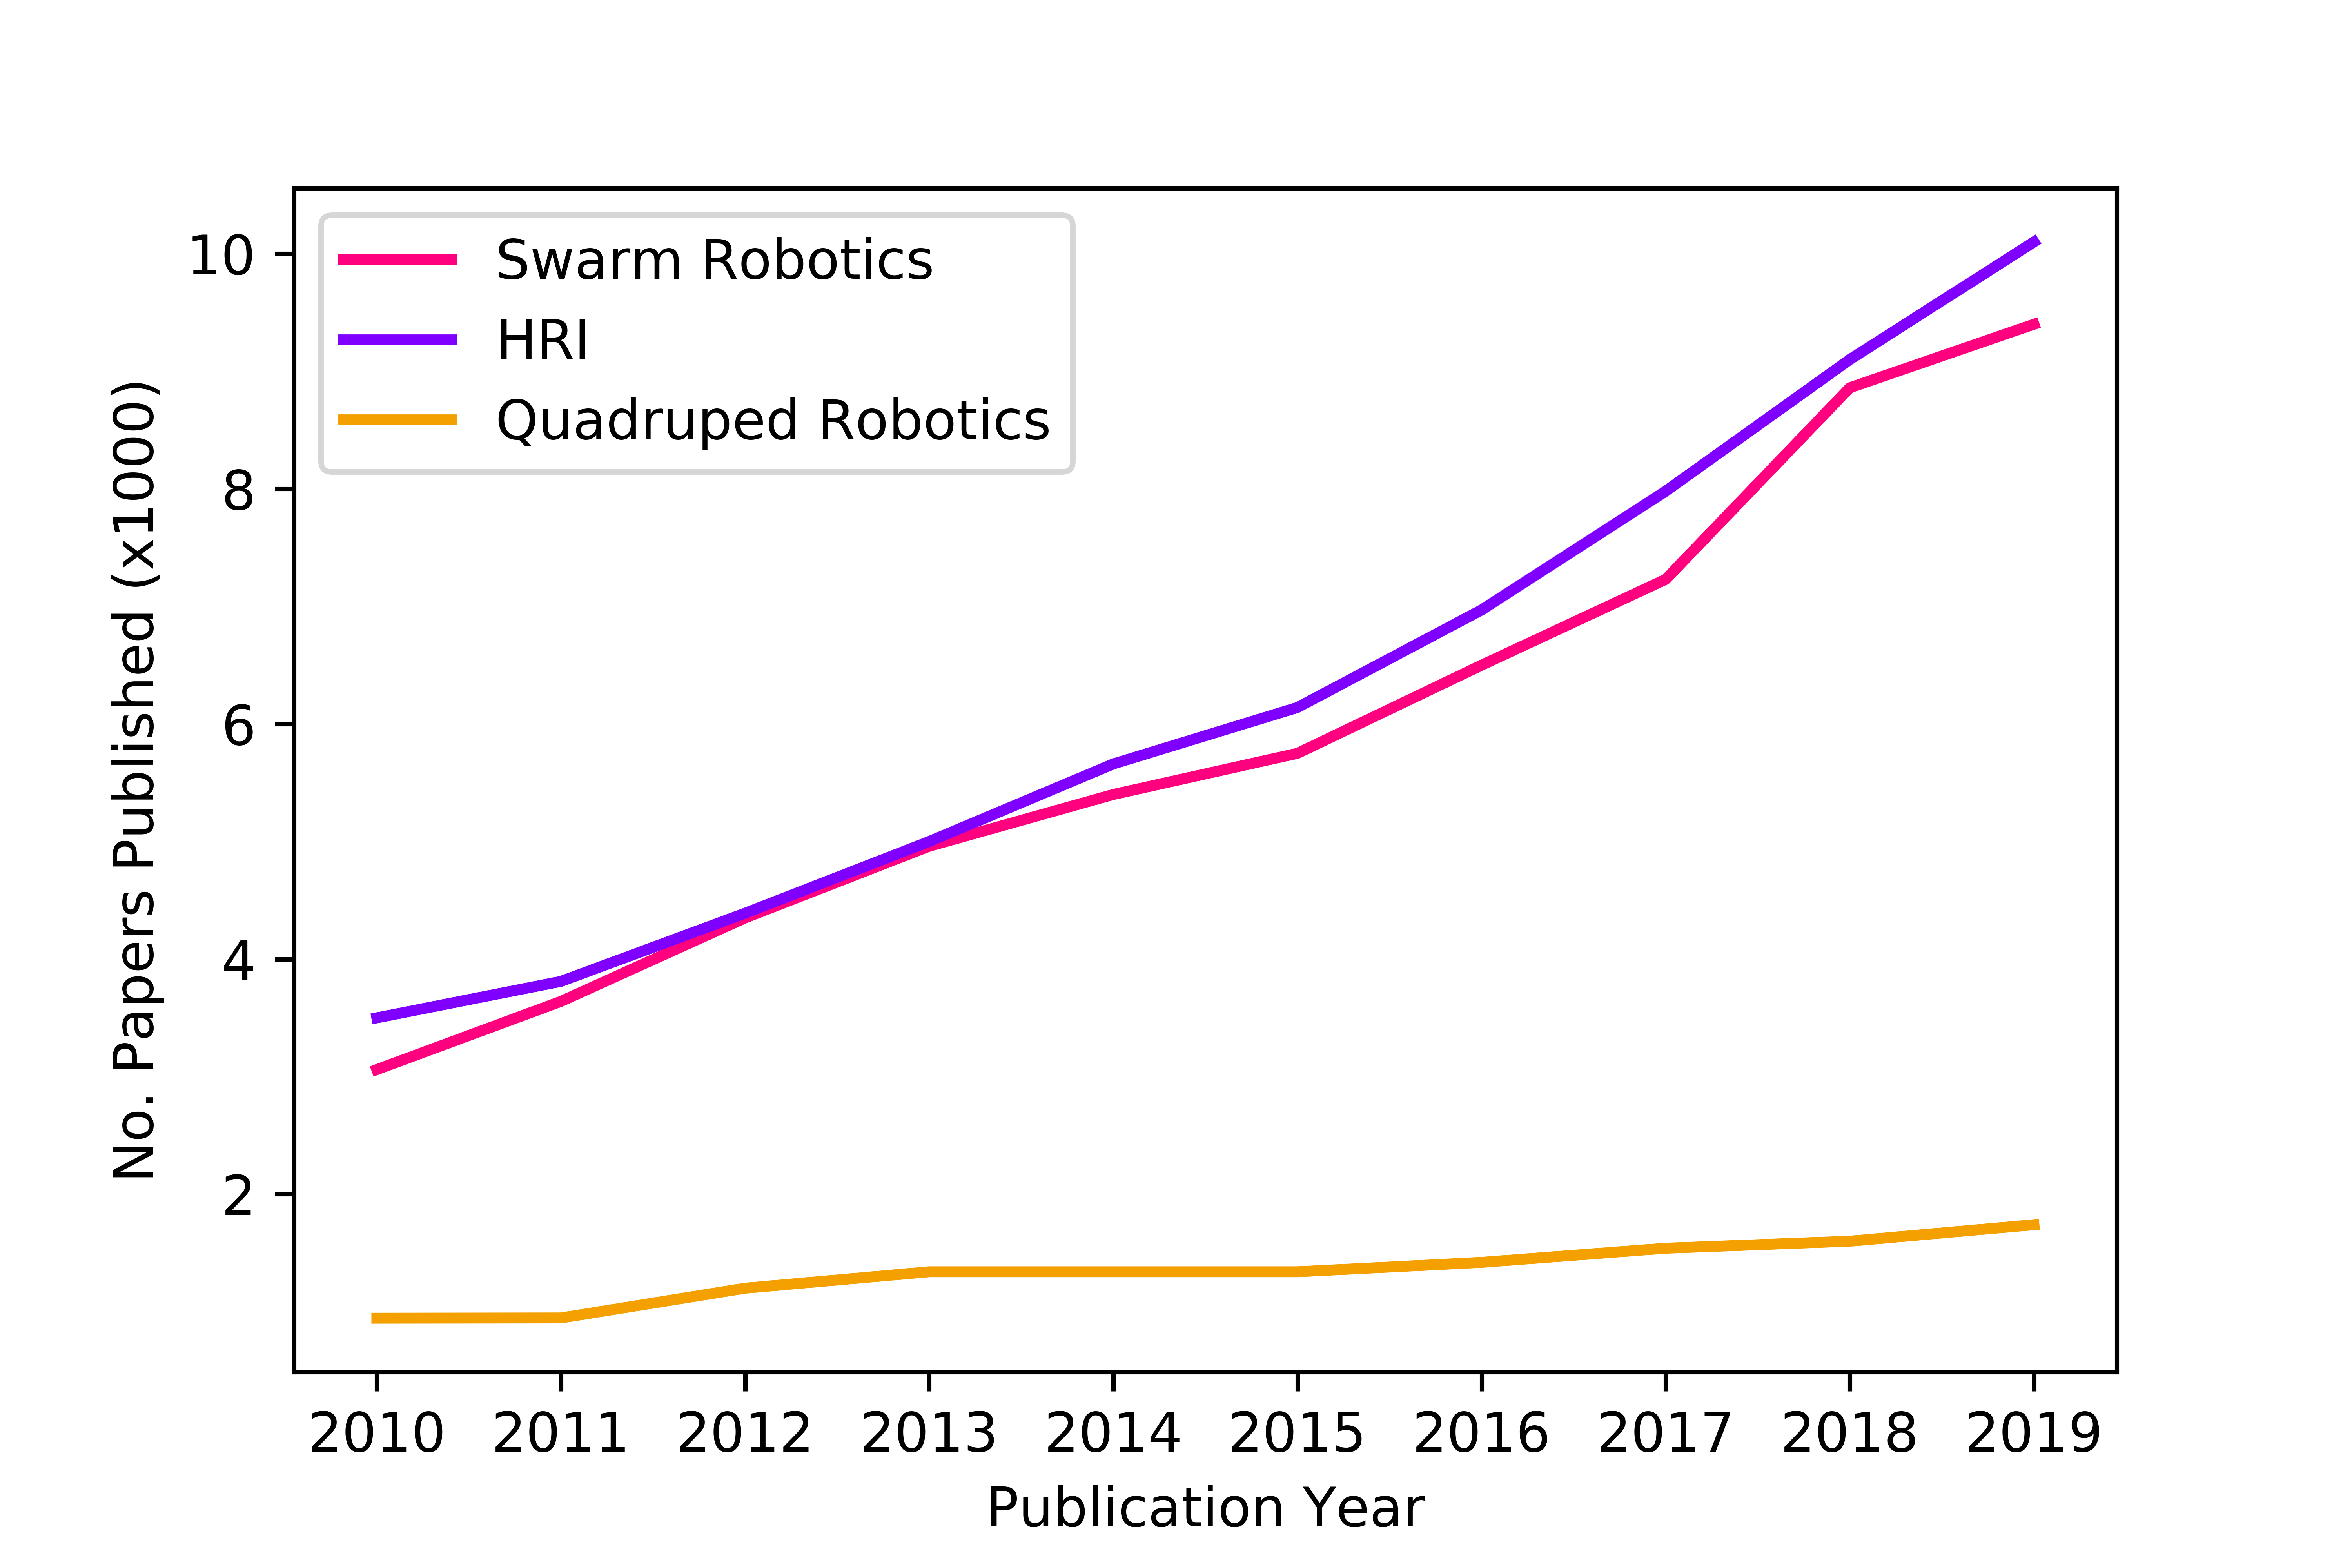
\includegraphics[width=0.49\textwidth]{Images/NumPapersPublished.png}
    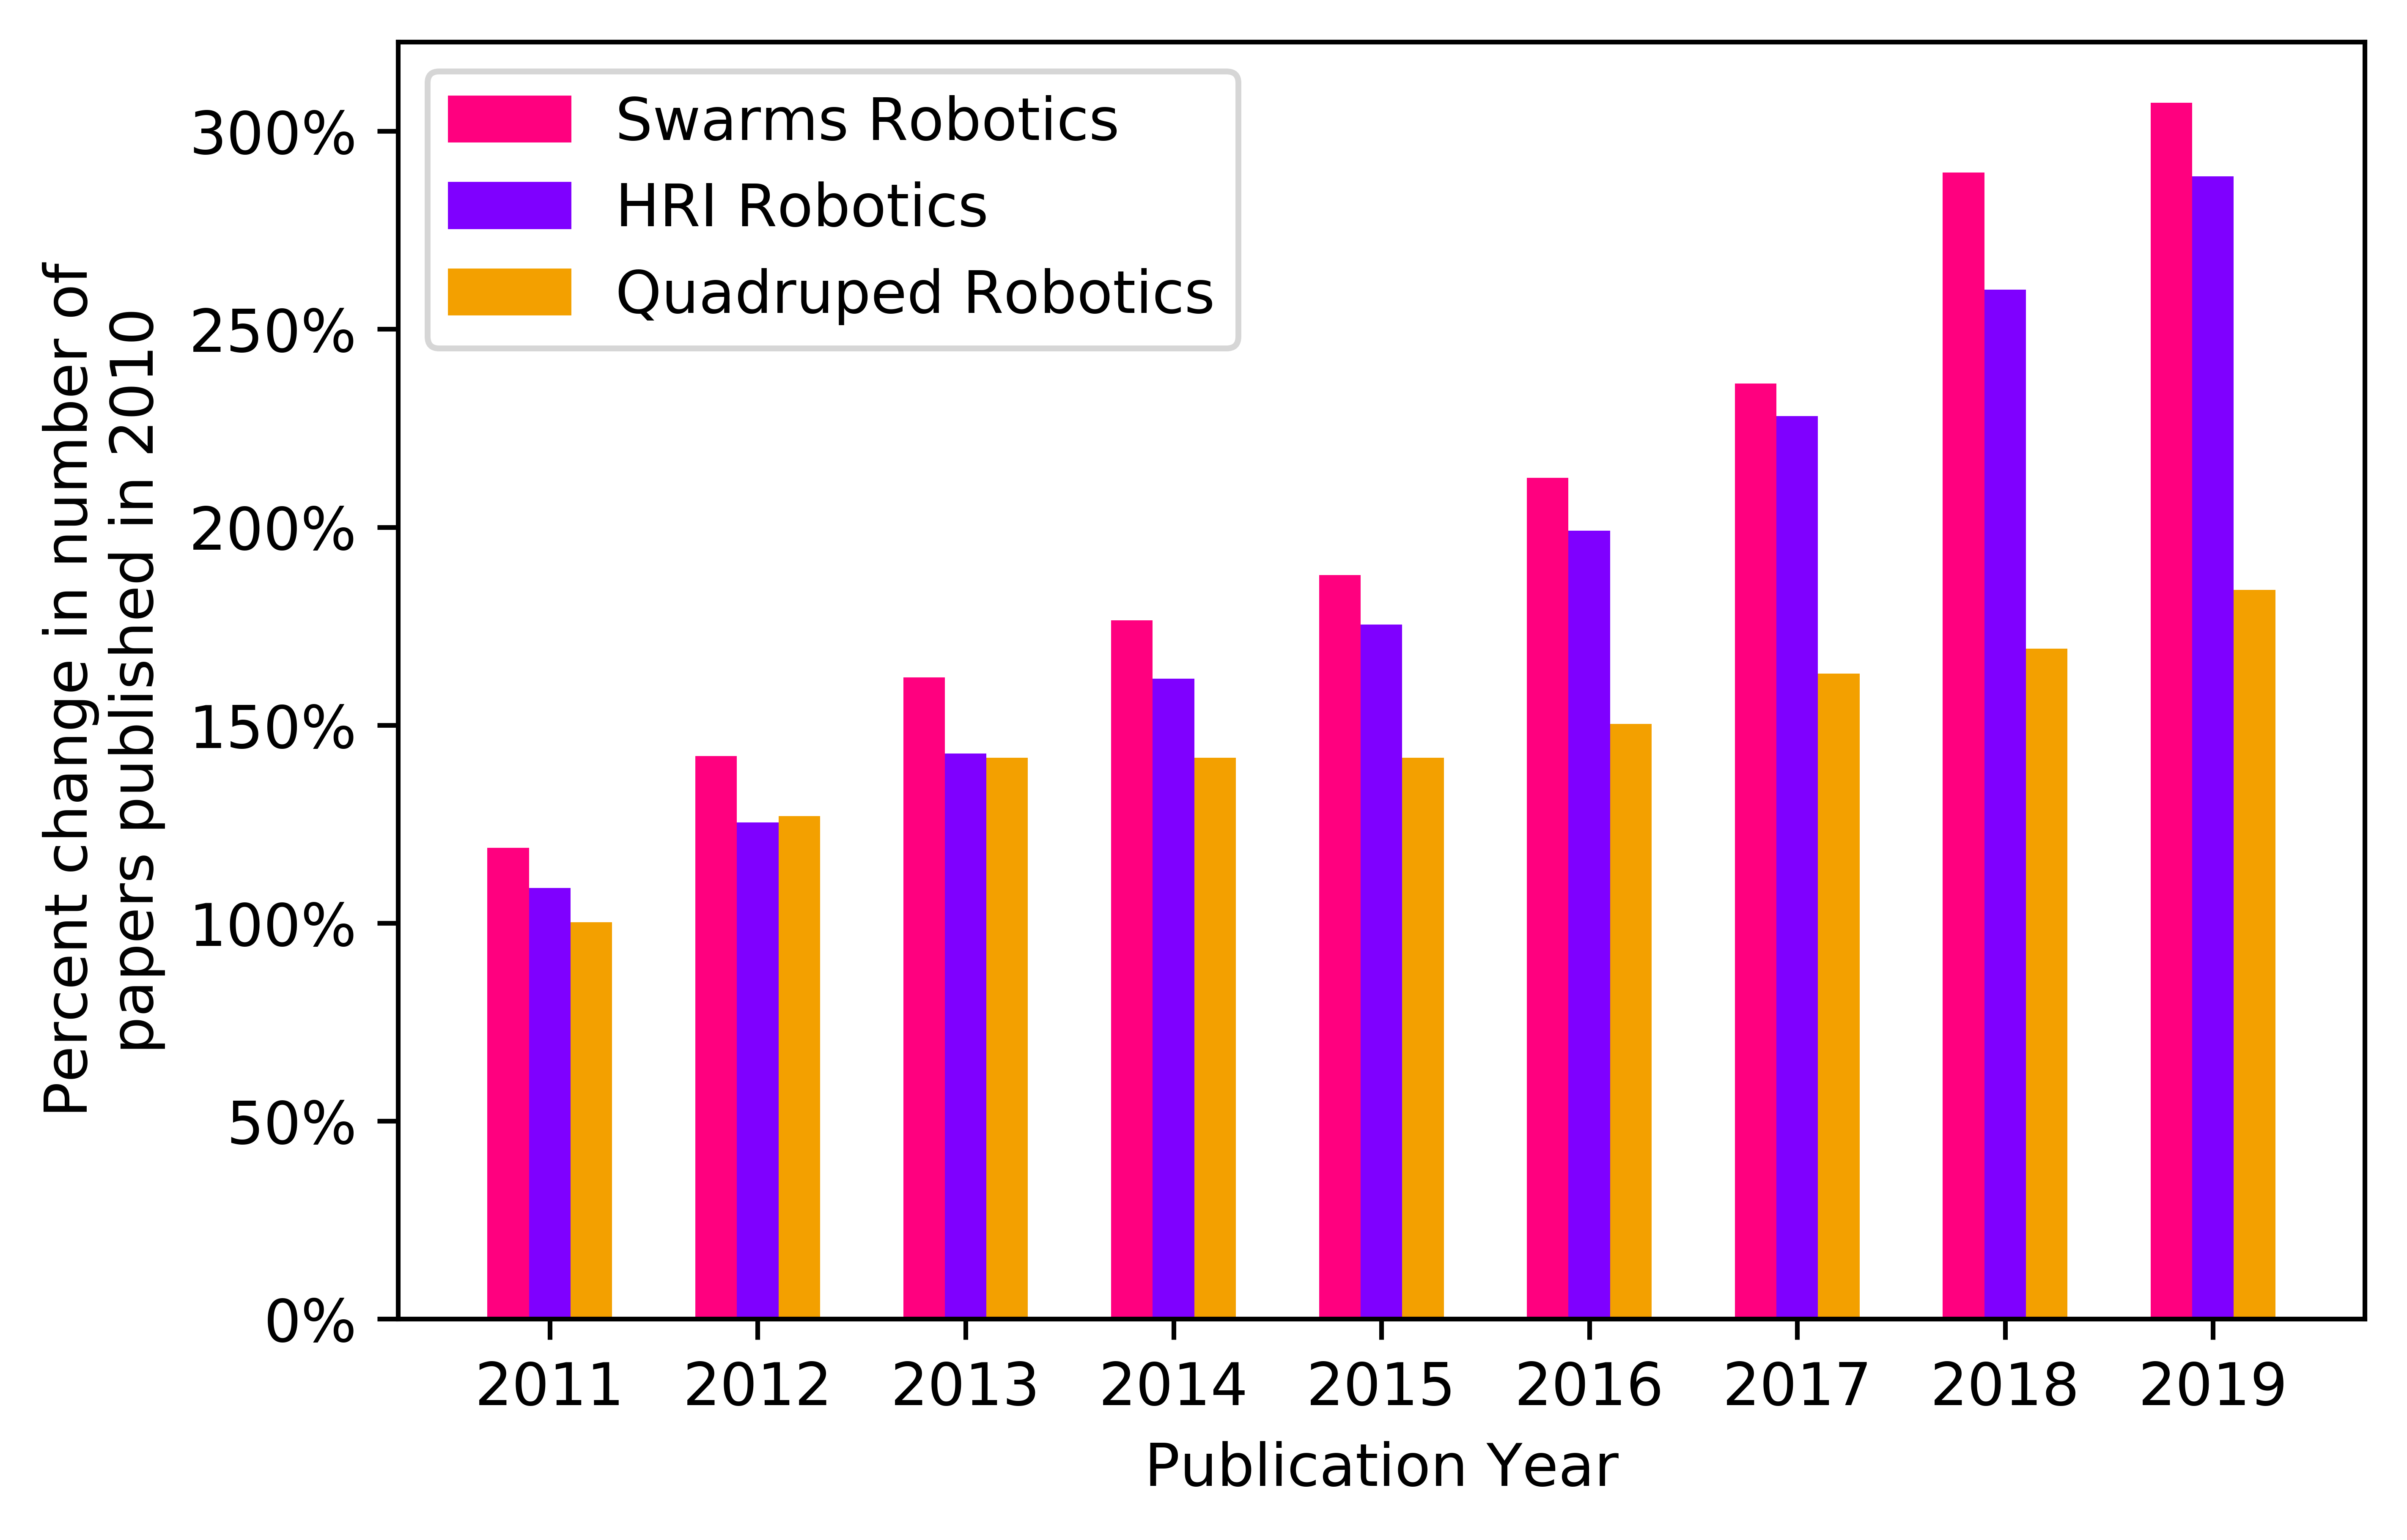
\includegraphics[width=0.49\textwidth]{Images/NumPapersPublishedDelta.png}
    \caption{Number of publications each year}
    \label{fig:comparison}
\end{figure}

From this data, it can be seen most university's offer courses in mobile robotics, Controls, Kinematics and Robot Manipulation. Very few universities offer courses in multi pedal systems with none offering labs to undergraduate students. This limitation on course concepts is likely due to the lack of available hardware and course concepts on the market. 

%%%%%%%%%%%%%%%%%%%%%%%%%%%%%%%%%%%%%%%%%%%%%%%%%%%%%%%%%%%%%%%%%%%%%%%%%%%%%%%%%%%%%%%%%%%%%%%%%%%%%%%%%

\chapter{Evolution of SmallKat}

\section{Origins}
The initial SmallKat robot was developed as an independent study project between 2 juniors over a 7 week term. This was done to explore the possibility of developing a quadrupedal robot capable of walking under its own power, with no supports for under \$200. The resulting robot can be see on the far left in Fig\ref{fig:Jaguar}. The final robot used 7g servo motors which proved to be very unreliable and had many issues in terms of performance due to these motors. T final design of the robot used a Teensy 3.5 micro controller for low level motor and sensor control in combination with a raspberry pi zero w for gait computation and development communicating through HID. This also proved to also have a number of issues due to the inconsistent HID support on the raspberry pi architecture. 
\begin{figure}[H]
    \centering
    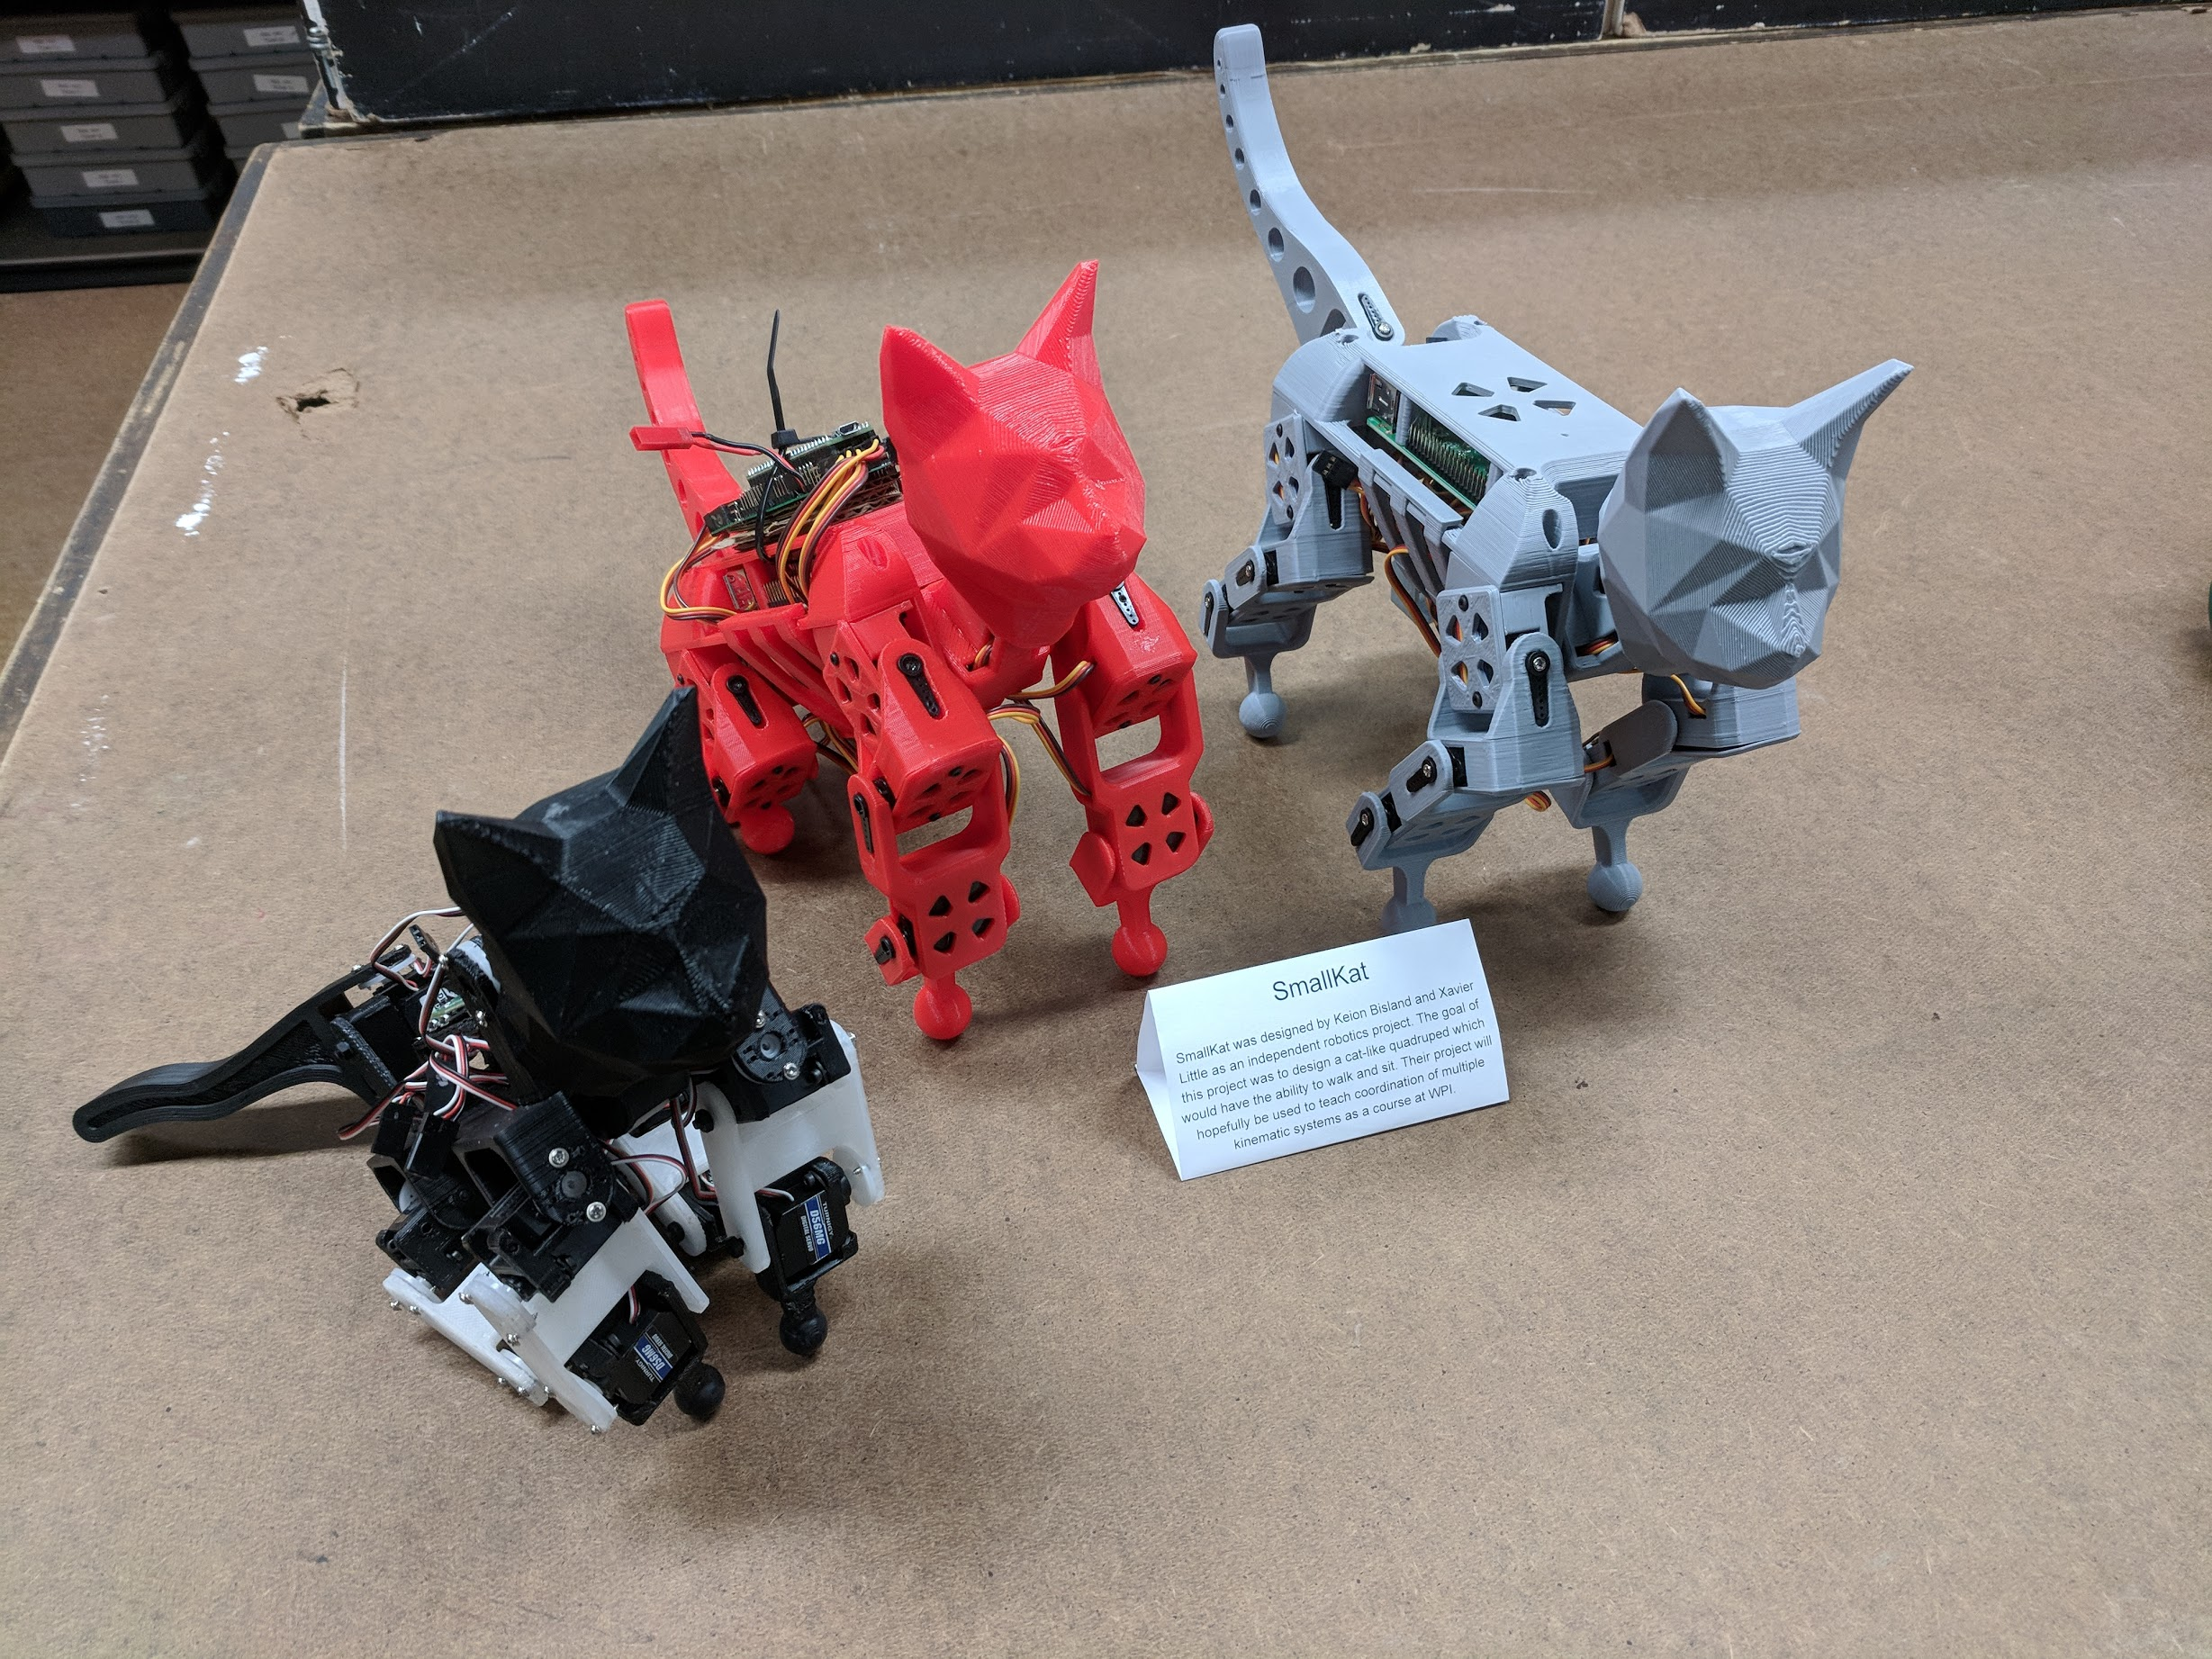
\includegraphics[width=0.5\textheight]{Images/V1andV2.jpg}
    \caption{1$^{st}$ Attempt: Jaguar (Far Left)}
    \label{fig:Jaguar}
\end{figure}

\section{1$^{st}$ Revision}
From all the first iteration, a number of things were learned; small servo motors are highly unreliable despite their high power to weight ratio, longer limbs allow for a more natural and  more efficient walking gait. In developing the second revision of the Smallkat robot, Grace, the servo motors were upgraded to more standard sized, metal geared 13g servos, the Tower Hobby-MG92B. These motors have a much higher torque rating that would allow us to make the limbs much longer without stalling the motors. The resulting revision can be seen in Fig\ref{fig:Grace}. This revision also came with a number of sensor and electrical upgrades including pressure sensitive feet which were tested but never fully integrated into the final walking gait. An IMU was also integrated into this revision using the BNO055 9DOF IMU, this gives a very accurate position and rotation of the body of the robot. This version did continue to utilize the Teensy 3.5 micro controller as most if not all early stage development was cone connected to a main computer for gait processing. Once the platform was developed further the ESP32 micro controller was utilized in order to have a reliable wireless communication to the robot in to communicate sensor data to the gait computation and motor data to the robot. 
\begin{figure}[H]
    \centering
    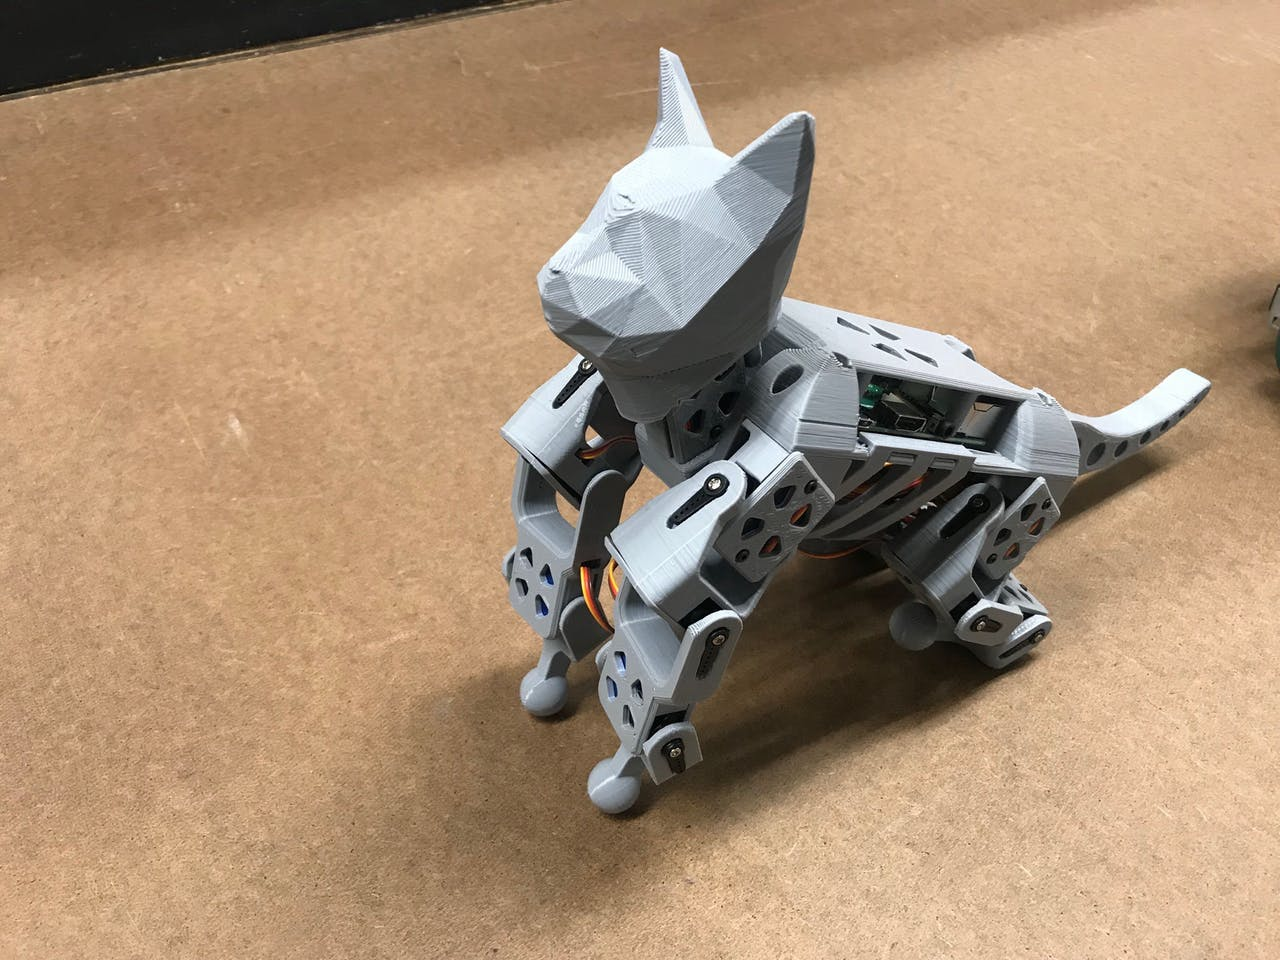
\includegraphics[width=0.5\textheight]{Images/1_sYQmYZO2XCQVxt3-icmhLw.jpeg}
    \caption{1$^{st}$ Major Revision: Grace}
    \label{fig:Grace}
\end{figure}

\section{MQP}
The purpose of the robot developed for the MQP was to explore the use of larger servos with more feedback as well as expanding the robot to have a 4$^{th}$ redundant DOF and a distributed computing system to lower the overall computation and execution time for the system. Having motors with \approximately32$\frac{Kg}{cm}$ of torque at each joint allowed the final robot, Fig\ref{fig:MQPKat}, to be much larger then previous iterations, these motors were developed as part of the project and Incorporated position, velocity and force control and feedback which would allow for a more dynamic robot with the potential of adding in compliance control for more unstable environment. The redundant 4${th}$ DOF was intended to allow for more dynamic and efficient gaits and will be explored further in this paper in Chapter \ref{chap:4Dof}. 
\begin{figure}[H]
    \centering
    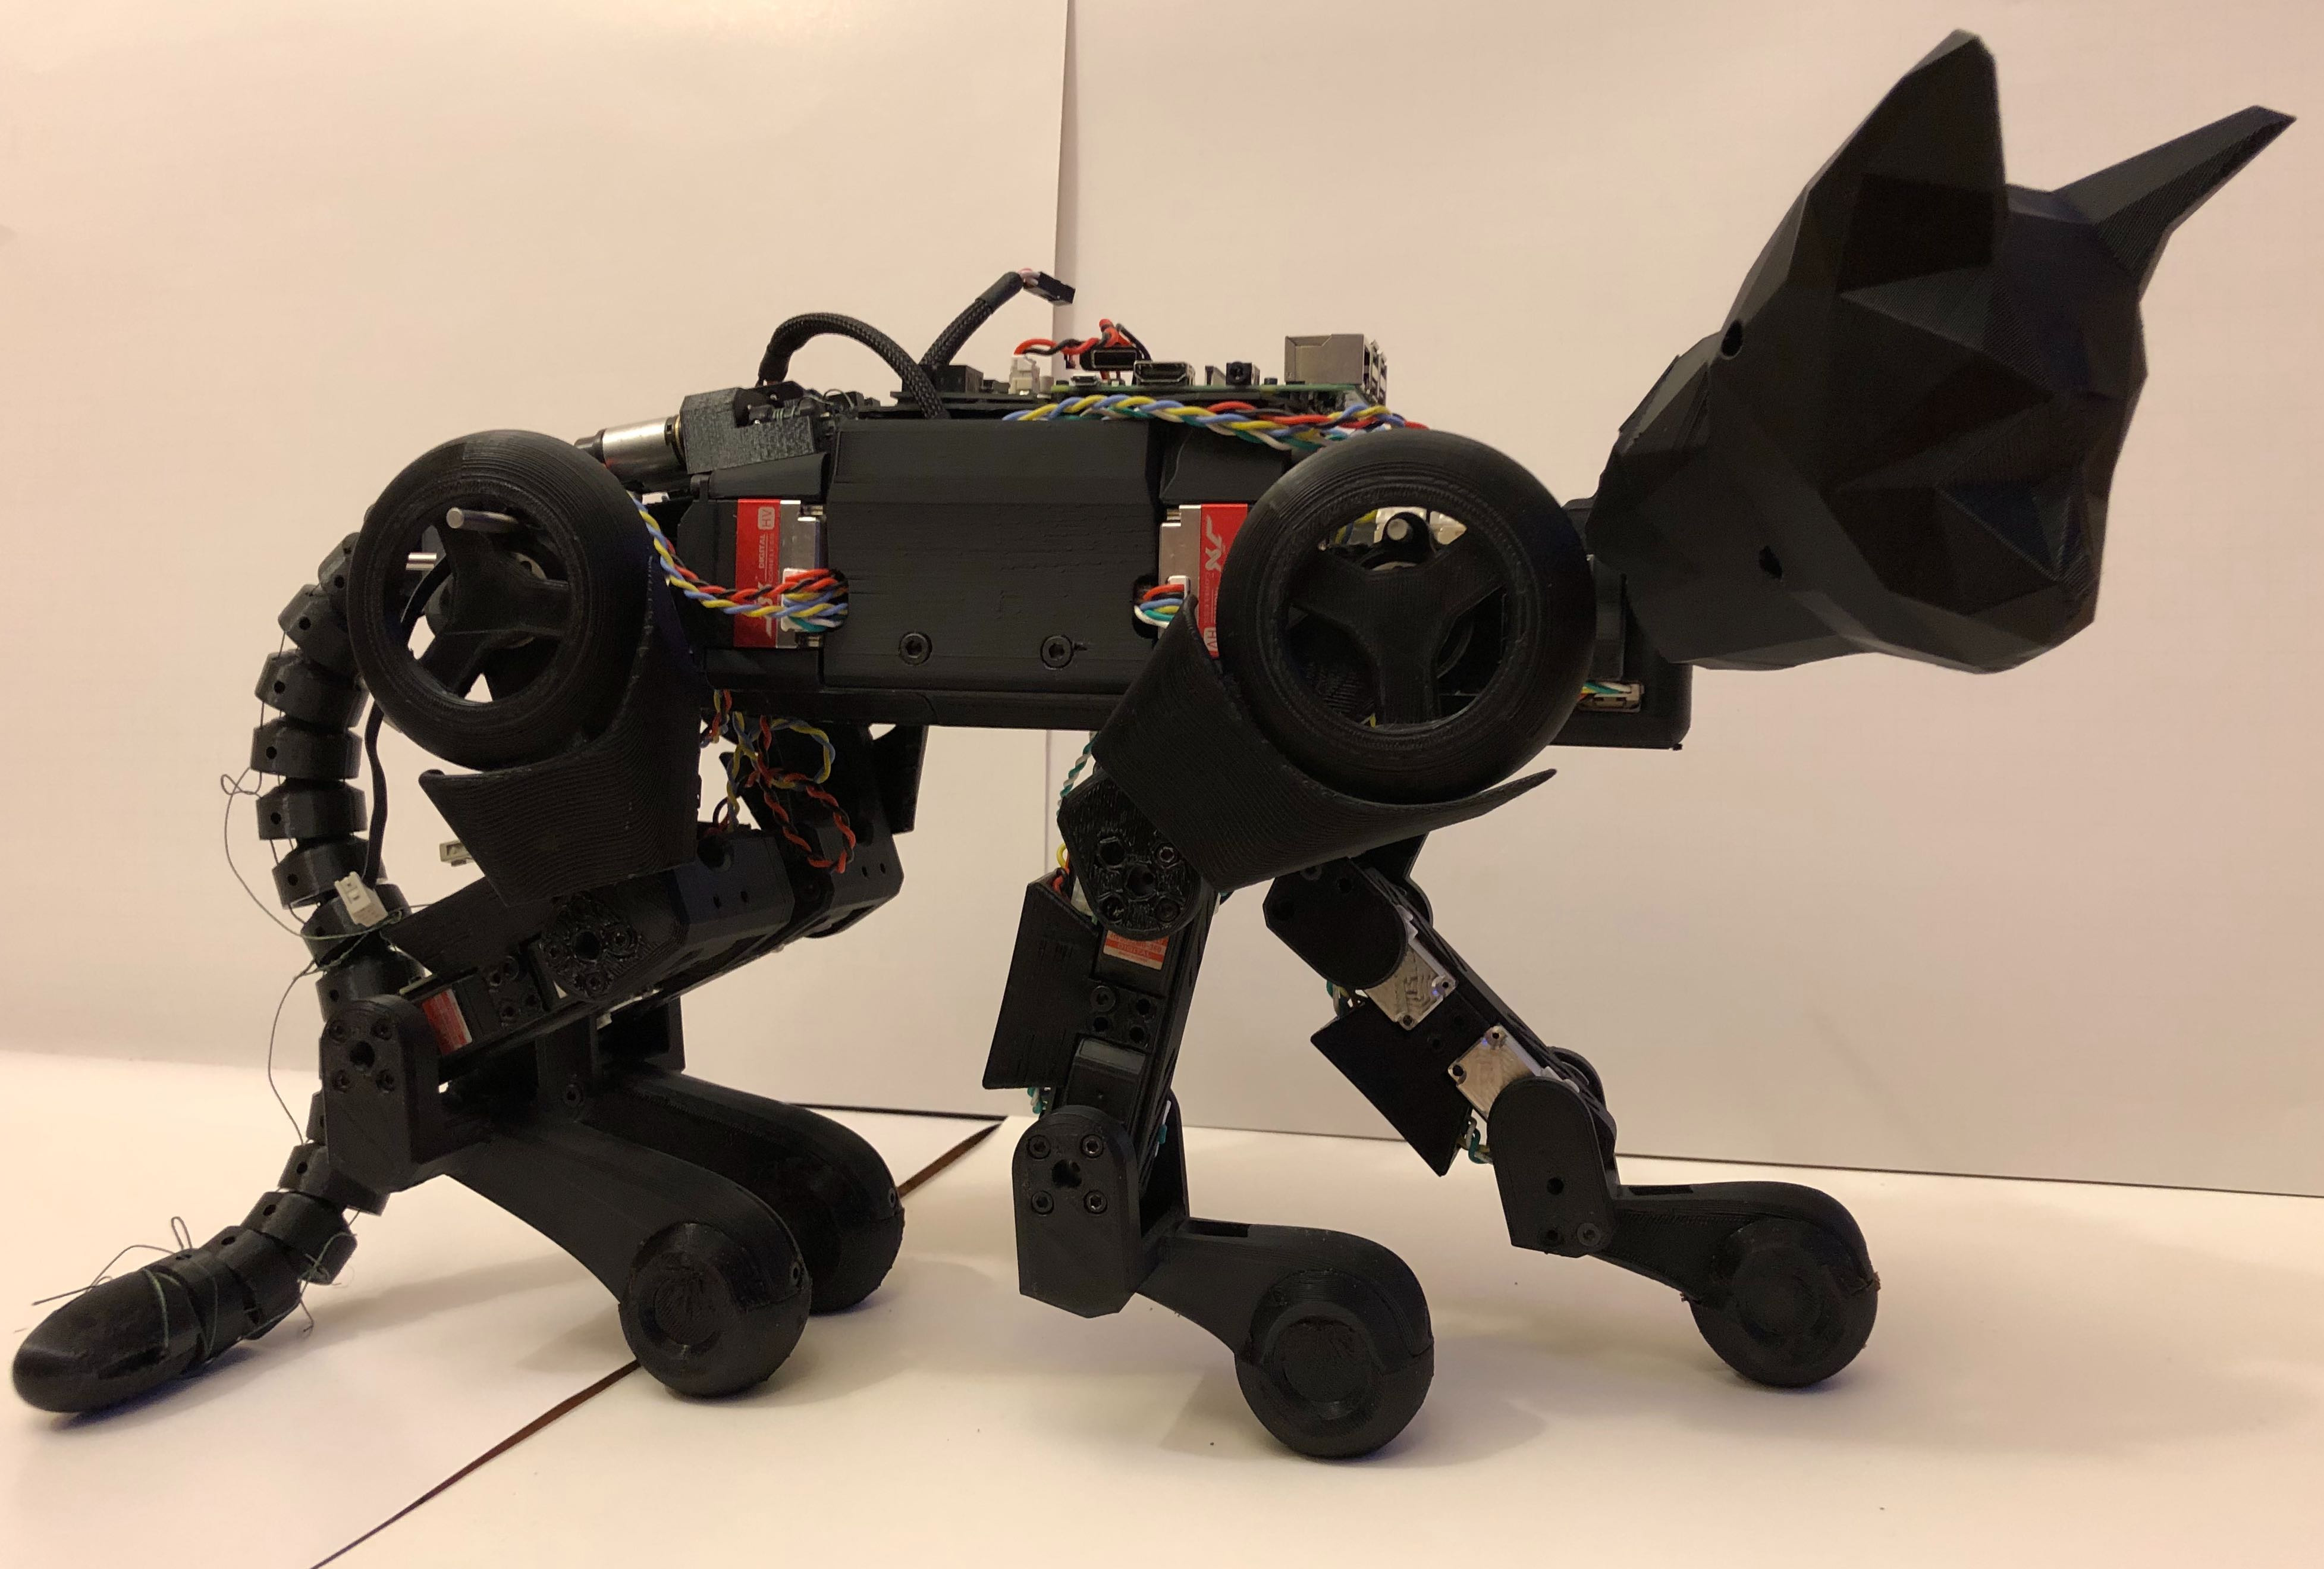
\includegraphics[width=0.5\textheight]{Images/FinalRobot.jpg}
    \caption{MQP Revision}
    \label{fig:MQPKat}
\end{figure} 

\section{Product Robot}
After all gained knowledge through the previous versions of the platform, a finalized version for the platform with the intention of use in education. The intended use for this platform would be to distribute a robot to each team of 3-4 students within a class to perform a series of labs pertaining to developing a dynamic walking gait while learning and improving abilities in kinematics, trajectory planning, controls and dynamics; all of which are integral parts of robotics. In order to do this safely, the platform must conform to a series of aspects elaborated further in section \ref{sec:DesignReqs}. The overall design and development process for this platform and the testing that was performed to ensure reliability and longevity in an abusive setting. The robot developed can be seen in Fig.\ref{fig:Luna}.  
\begin{figure}[H]
    \centering
    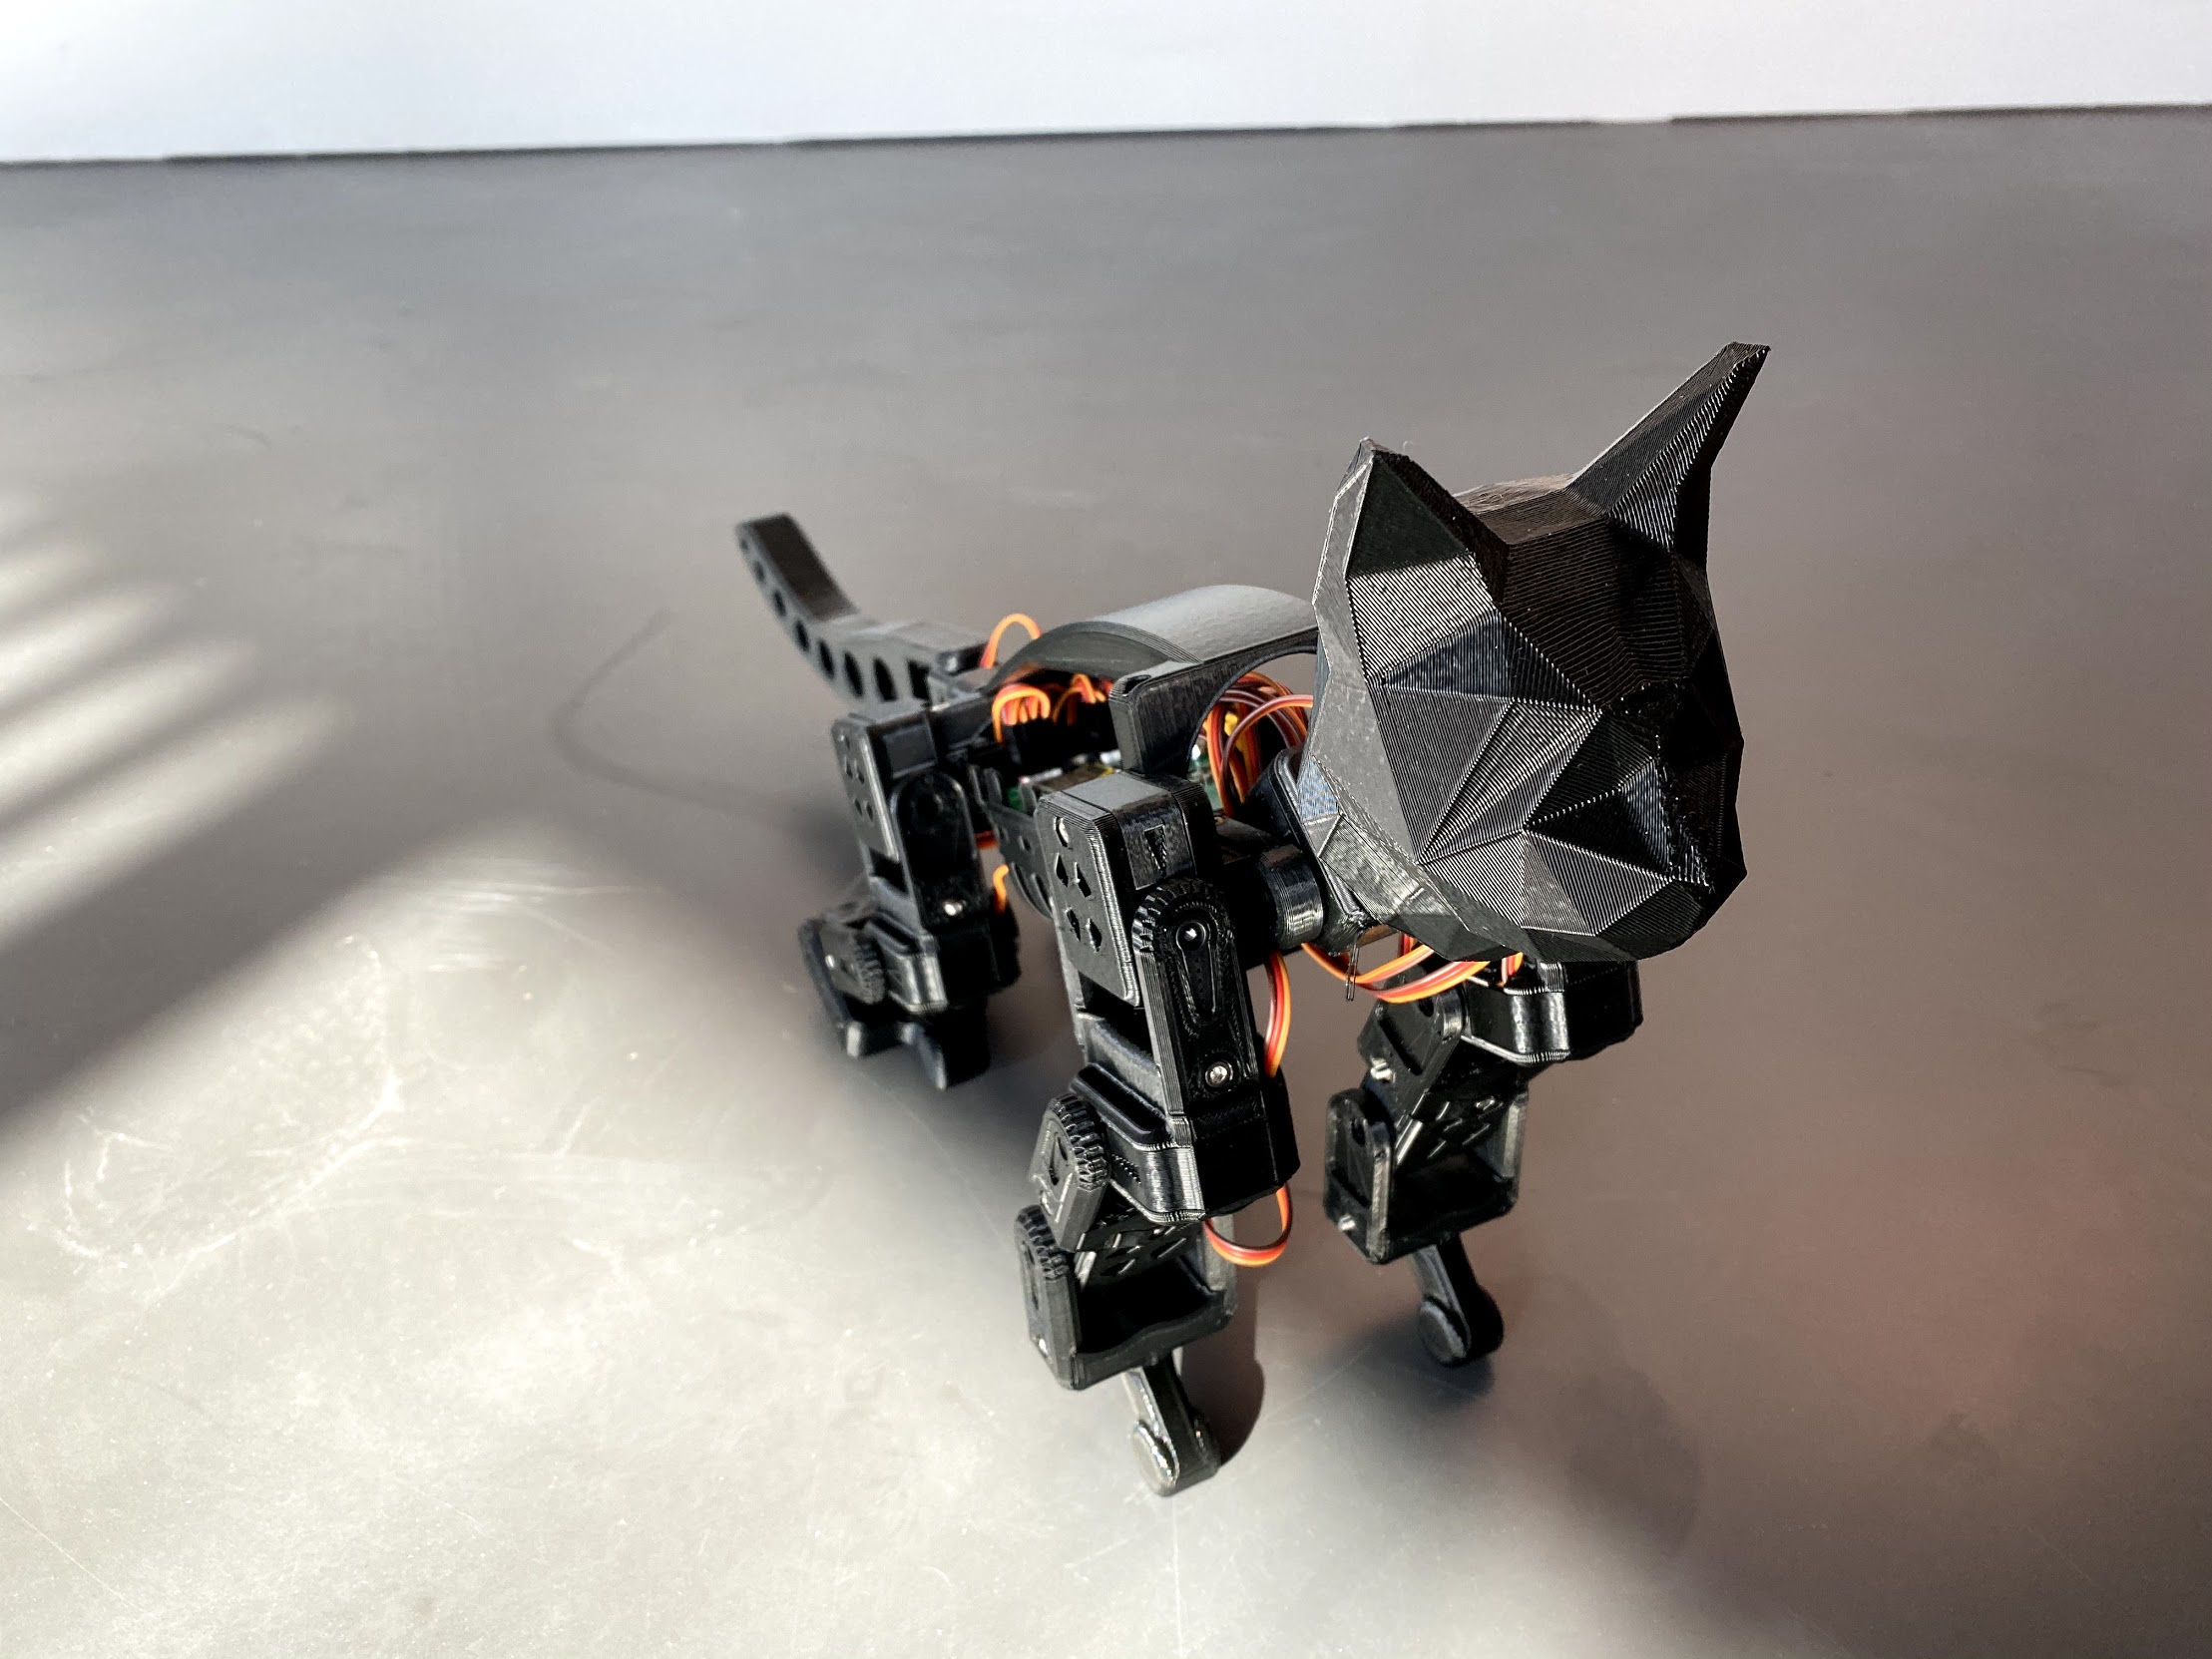
\includegraphics[width=0.5\textheight]{Images/IMG_0119.jpg}
    \caption{Product Revision: Luna}
    \label{fig:Luna}
\end{figure}
%%%%%%%%%%%%%%%%%%%%%%%%%%%%%%%%%%%%%%%%%%%%%%%%%%%%%%%%%%%%%%%%%%%%%%%%%%%%%%%%%%%%%%%%%%%%%%%%%%%%%%%%%

\chapter{Development for Teaching}
\begin{hyp}[H\ref{hyp:first}] \label{hyp:first}
A platform capable of performing all aspects needed to effectively teach quadruped dynamics and supporting topics could be developed at a price point similar to that of the turtlebot burger (\$550)
\end{hyp}
\begin{itemize}
    \item[-] Can a quadruped robot be designed to safely operate in a class setting?
    \item[-] Can a quadruped robot be designed for quick assembly \& mass production?
    \item[-] Would the addition of a redundant 4$^{th}$ DOF make the robot better?
    \item[-] Can a quadruped course and lab be developed for an undergraduate student level?
\end{itemize}
\section{Design Requirements}\label{sec:DesignReqs}
    In order to design the platform appropriately the teaching objectives had to be defined and considered in the development process. The sections proceeding cover all the topics covered and their relationship to the platform.
    \subsection{Kinematics}
        In learning control and manipulation of a multi DOF system, Kinematics and Denavit–Hartenberg parameters are crucial. Through this series of equations and parameters all following concepts can be taught and tested sufficiently. A strong understanding of these concepts is crucial for any multi DOF and/or multipedal system.
        \subsubsection{D-H Parameters}\label{DH-Params}
            D-H Parameters explain the configuration of each joint of the robot and its translation from the previous join tin a series of 4 Parameters. Through these parameters the forward kinematics of the system can be quickly and easily computed with very little modification in the case of a change to the system. Table \ref{tab:DHParametersLeg} shows the DH Parameters of the legs of the robot.
            
        \subsubsection{Forward Kinematics}
            Forward Kinematics are the calculations of the end-effectors position in the X,Y,Z work space given the current joint angles. this can be approached in 2 ways.
            
        \subsubsection{Inverse Kinematics}
            Inverse kinematics are used to calculate the joint angles required to reach a certain target goal in the work space. These joint angles can be derived from a series on equations.
           
    In order to cover topics so important to the material for the course it was imperative that the kinematics for the system could be developed and tested on a single leg before testing on the whole robot. This was achieved through software integration allowing for individual joint control from the high level interface. This allows the users to develop and test their kinematic equations in a reliable way in order to get a solid understanding of the concept.
    
    \subsection{Trajectory Generation}
     Following kinematics and preempting gait generation the topics involved in trajectory planning are of high importance. Understanding frame transformations and $n^{th}$ degree polynomials for path and trajectory generation will make the process of gait generation and motion planning far easier and more efficient. 
    
    \subsection{Gait Generation}
     Following Trajectory generation comes gait generation. This covers the trajectories that must be followed for each leg in a specific sequence in order to achieve a specific body trajectory, moving the entire robot in a specific direction.
    
    \subsection{Controls and Dynamics}
      When developing a complex system controls and dynamics are crucial to have the robot accurately and safely perform tasks and actions commanded to it. The platform must be able to have both control systems and dynamic controllers implemented to account for external input from the environment.
%%%%%%%%%%%%%%%%%%%%%%%%%%%%%%%%%%%%%%%%%%%%%%%%%%%%%%%%%%%%%%%%%%%%%%%%%%%%%%%%%%%%%%%%%%%%%%%%%%%%%%%%%
% \chapter{System Architecture}
\chapter{Mechanical Redesign}
When designing the mechanical system for the robot, there were large number of constraints to overcome. Many of the constraints can be refined down to the cost and the size constraints set forth during the development of the platform. 
    \begin{itemize}
        \item Motor selection- 
            When deciding motors to use there were a number of criteria to compare: Size, Torque, Power requirements and Availability.

            In end the 13g servo form factor was chosen for the size as it would allow the overall robot size to remain small and light. It then came to choosing the specific motor to use, it came down to 4 motors. Due to sharing the same form factor they all remained in a very similar volumetric size so the decision came down to which motor would be most capable and reliable. After testing with all of the considered motors, the final motor chosen was the TowerHobby MG92B for its high size to torque ration, being far higher than the other options as well as its availability from many distributors around the world.\newline
        \item DH Parameter Optimization
        In order to optimize the DH parameters and in turn the overall design of the robot the torque jacobian for each of the legs was computed and  values were tested iteratively to achieve a torque of less than 3Kg/cm in the least optimal case. This resulted in the DH parameter in table \ref{tab:DHParametersLeg} where link 0 is the translation from the center of the body to the first joint for each leg. 
        \begin{table}[H]
            \centering
            \begin{tabular}{|c|c|c|c|c|}
            \hline
            Link& A  & $\alpha$ & D & $\theta$ \\
            \hline     
                0 &  $\pm$151.42 & 0 & 0 &0\\
                1 &  45.50 & $-\pi/2$ & 0  &$\theta_1$\\
                2 &  55.50 & 0& 0 & $\theta_2-\pi/4$\\
                3 & 60  &0 & 0  &$\theta_3+\pi/2$\\
            \hline
            \end{tabular}
                \caption{\label{tab:DHParametersLeg}D-H Parameters of a single leg}
        \end{table}
        \item Manufacture-ability
        While designing this robot a great deal of time was spent in designing for manufacture-ability. Each method of manufacturing has different constraints in what can be produced successfully, efficiently and quickly. When designing a number of factors were considered. Manufacturing style, Number of components and Production cost
        The primary means of manufacturing was chosen as 3D printing because it would allow the robot to be iterated quickly and available to the most people. However for mass production of the platform, a series of molds would be created and parts would be cast using a poly-urethane resin. This required all parts to be designed with both manufacturing styles requirements in mind ensuring there were as few areas with unreachable overhangs, parts could be placed flat in order to reduce the amount of support material while printing and many other details. By choosing these two methods of manufacturing the overall production costs are kept very low.\newline
        Due to the nature of the system, there will be a high number of individual components (79 total parts in the final design), by reusing the same piece in multiple it both reduces the complexity of assembly and the total number of models that have to be manufactured. Through this technique, the robot was able to be designed out of 22 unique components which would be able to be printed in 3 cycles of a standard 200mm x 2000mm 3d printer (industry standard for consumer printers).\newline
        \item Assemble-ability
        While manufacture-ability encapsulates the majority of the design process, the means of assembling was also considered carefully. The ability to put the robot together quickly and easily is critical. By analyzing the process taken to assemble an early prototype of the robot and adjusting the design the assembly time was reduced from \approximately 5hrs to \approximately1.5hrs. The final revision of the design utilized 2 lengths of m3 bolts and their corresponding nuts to assemble the whole robot. The use of 2 lengths of screws also drastically reduces the cost. 
        
    \end{itemize}
    
\chapter{Electronics Redesign}

The electrical system of the SmallKat platform incorporates a number of features including a main micro controller, a high current an highly reliable power regulator, a 9 DOF inertial measurement unit with a high level of accuracy as well as a number of safety features integrated to ensure reliability and consistency of the platform. An overview of the electrical architecture can be seen in Fig. \ref{fig:elecpic}

\begin{figure}[H]
    \centering
    \begin{tikzpicture}[]
        % Place nodes
        \node [block] (PSU) {Power Supply};
        \node [block] (ESP) [below =0.5cm of PSU]  {Main MCU};
        \node [block] (LPC) [below right =-0.3cm and 0.75cm of ESP] {Safety MCU};
        \node [block] (CHG) [right =0.75cm of PSU] {Charging};
        \node [block] (IMU) [below =0.5cm of ESP] {IMU};
        \node [block] (Servos) [left =0.75cm of ESP] {Servos};
        % Draw edges
        \path [line] (PSU) -| (Servos);
        \path [line] (IMU) -- (ESP);
        \path [line] (LPC) |- (ESP);
        \path [line] (ESP) -- (Servos);
        \path [line] (LPC) -- (CHG);
        \path [line] (CHG) -- (PSU);
    \end{tikzpicture}
    \caption{Overview of the Robots Electrical System}
    \label{fig:elecpic}
\end{figure}
    \begin{itemize}
        \item Micro controller -
            When choosing the micro controller there were a few requirements set forth, it would have to be able to run 16 independent PWM signals, communicate through either USB-HID or UDP and have a hardware $i^2c$ channel.
            \begin{enumerate}
                \item Teensy 3.5/3.6
                \item Teensy 4.0
                \item ESP32
                \item STM32
            \end{enumerate}
            From currently available microcontrollers, a custom motherboard was developed. From these micro controllers it was narrowed to either the Teensy 3.5 or the ESP32, one option providing hardware USB-HID and the other UDP over WIFI. From this a final version of the motherboard was developed using the available boards. Both boards were then tested thoroughly.\newline
            
        \item IMU- 
            The IMU chosen was the BNO055 as it filters the data returned by the IMU. This allows the system to have a much more reliable source of feedback. The IMU is also able to provide a gravity vector and the Euler angles within each axis of rotation.\newline
            
        \item Power regulation-
        Due to the power requirement of the motors chosen, a consistent 6v power supply with about 20A continuous current draw is required. 6v is a very uncommon voltage supply with 2s lithium batteries coming in at a nominal 7.4V and most bench power supplied only supplying a maximum of 10A. In order to increase the battery life capacity without increasing the size of the cells as well as allowing for higher voltage power supplies with lower current ratings to be used a high current switch mode supply was designed with up to an 48V input and up to 30A output. With an overall efficiency of about 85\% with a 20A draw the onbaord supply is highly efficient at converting high voltage, low current supplies down to 6v at the required 20A. \newline
    \end{itemize}
    During the development stages of the motherboard, off the shelf development boards and modules were used for the micro controller, IMU and power regulation. This drastically increased the overall cost of the electronics in the system. Once the system was proven and tested, the final revision of the motherboard was designed and resulted in a cost reduction of about 80\%. In addition to the cost reduction, The overall number of through hole components was drastically reduced, making it marginally easier to produce.
%%%%%%%%%%%%%%%%%%%%%%%%%%%%%%%%%%%%%%%%%%%%%%%%%%%%%%%%%%%%%%%%%%%%%%%%%%%%%%%%
\section{Electronics Validation}

\subsection{Testing Fixture}
In order to endure reliability of the developed motherboard and controller board a series of exposed test points along the reverse of both boards were placed in order for the board to be placed on a test fixture to confirm all the major sections of the board are working. The test points test the USB programming circuit on both boards, the $i^2c$ lines, a micro controller working pin and 3.3v is tested for both the mother board and the controller board. In addition to these, on the motherboard the ere are probe points to inject battery voltage, inspect the out put voltage for the integrated switch mode regulators and the battery voltage sense circuit. in order to easily and quickly test these boards a mirrored board was developed using spring loaded pins with a micro controller and serial programmers onbaord. A fixture that this board is mounted into was then designed and 3D printed to allow for quick insertion and removal of the board under test. A series of leds was added to act as confirmation lights with different ones turning on or off for different things under test for each board. The testing procedure can be seen in appendix[\ref{appendix:TestingProcedure}]

\subsection{Safety}
    In designing the system, great caution had to be taken with the lithium ion battery in the system. In order to keep the system safe, a series of fuses were integrated into the motherboard to prevent from short circuits or failures of motors. In addition to this current sensors have been added to each motor to determine major stall states to prevent complete failure of the motor. In addition to these a secondary micro controller was implemented as a safety system. This micro controller will monitor battery voltage, charge state, battery charging and battery balancing to ensure each cell is evenly charged to ensure longevity and safety. This micro controller will also  maintain control over the onboard power regulators and will be able to turn them on or off in a series of cases. This micro controller will remain on and in low power mode while the robot is turned off or the battery is too low to be used safely. In order to safely charge the battery pack, a charging system utilizing USB power delivery was implemented along with a cell balancing and monitoring system. chapter{Mechanical Redesign}
\subsection{Testing Procedure}
\label{appendix:TestingProcedure}
\begin{enumerate}
    \item Plug in both USB cables for ESP32 programmers on jig
    \item Plug in communication USB for onboard micro controller
    \item Run Python test script
    \begin{enumerate}
        \item Program controller board with test firmware
        \begin{enumerate}
            \item Test for 3.3v regulation, $i^2c$ communication and micro controller status
            \item If passed program with final firmware
        \end{enumerate}
         \item Program Motherboard with test firmware
         \item Enable Battery power input
        \begin{enumerate}
            \item Test for 3.3v regulation, 6v regulation and battery monitoring circuit
            \item Test $i^2c$ communication to the micro controller
            \item Test $i^2c$ communication to the IMU
            \item Check micro controller status
            \item If passed program with final firmware
        \end{enumerate}
    \end{enumerate}
    \item Display a Pass/Fail status of the board, with reason of failure    
\end{enumerate}
%%%%%%%%%%%%%%%%%%%%%%%%%%%%%%%%%%%%%%%%%%%%%%%%%%%%%%%%%%%%%%%%%%%%%%%%%%%%%%%%%%%%%%%%%%%%%%%%%%%%%%%%%

\chapter{Software Redesign}
\section{Language Choice}
In choosing the language, development environment and in turn some of the electronics and hardware, a number of things had to be considered. A prime focus came down to choosing the programming languages used to develop both at the high level on the main processing and the low level on the micro controller. Each of these come with a varying list of potential languages. So in order to determine which language should be chosen, a list of programming languages at both the high level and low level were devised and can be seen here: the primary list of languages for this High level control development include C/C++, Java, Python, Matlab and GO. This same procedure was performed for the low level programming language to be used on the micro controller. This was used to compare primarily C/C++ and micro python.  
    \begin{figure}[H]
	\centering
      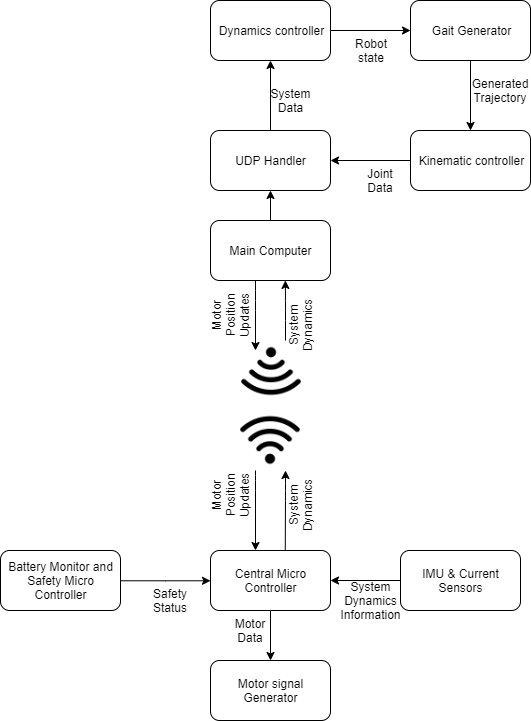
\includegraphics[width=0.65\textwidth]{Images/SmallKatControllerDiagram.png}
  	\caption{System Control Diagram}
  	\label{fig:controStructure}
\end{figure}
\subsection{High Level Control}
When choosing the language for the high level programming language, a number of considerations were made. The operation support off each language being of high importance as all computation and communication should ideally be systematically agnostic. From there the development speed and run time speed were analyzed for each language as well as the commonality of the language to aid in development and education. 

\subsubsection{Language Commonality}
    In order to get a platform adopted the language used needs to be common and well supported, this therefor brings the list of languages down to Java, C/C++, Python and Matlab. These three languages encapsulate the top 48\% of most popular programming languages\cite{tiobe}. This leans they have a great deal of documented and community support and therefor can be debugged and developed easily.

\subsubsection{Operating System Support- High Level Control}
    While most languages are supported by Mac OS, Linux and Windows, some are far easier to compile and get working than others. In order to make the start up process as easy and seamless for the end user, a language that could be pre-compiled or did not require specialized packages to compile would be chosen. This reduced the language choice for the high level controller to either Java, Python or Matlab.
    
    Due to the requirement of a Matlab license to use the program to its full potential it was eliminated. 
\subsubsection{Development speed}
    With the nature of classes and labs, development time and learning curve is a key concern, students should be learning the concepts of the class and not a new language. In this Python is the clear leader, it has the lowest learning curve as well as the lowest development time. However Java has a number of scripting languages such as Groovy, Kotlin and PyJava. These drastically reduce the development time of java while still allowing the user to integrate pure java code with out issues at compilation and run time. Meaning both Java and Python are strong language contenders int his regard.

\subsubsection{Run time speed}
    In order to get a reliable dynamical controller run at a high level it was important to have language that could have full system resources allocated to it. It was also important that the language was able to run in a real time-esq system where a set of code could be run on a high frequency interval with reliability and this could be done on any system without having an effect from other code. In this case Java was the final choice as the `Niceness' of the program could be adjusted to prevent other system processes from affecting the run time of the program. This in combination with the object oriented nature of the language makes development and implementation of features very easy for the instructor and students.\newline


Due to all of these considerations Java was chosen as the primary language for back end development and for script and gait development a Java based scripting language called Groovy will be supported, however any java based scripting language will work and/or Java itself will work in the same manner. \newline

\subsection{Micro-Controller}
When deciding the language to use for micro controller development a number of factors such as environment setup, language functionality and library support. These criteria were analyzed for both micro-python and C/C++ in a variety of environments. 
\subsubsection{Micro-Python}
    Micro Python is an implementation of python developed for micro controllers, running naively on board. Using micro python comes with all the benefits of python such as the ease and speed of develop-ability but also comes with many draw backs as it can be less efficient than some of its counterparts. Configuring the ESP32 to run Micro Python requires quite a bit of effort to be put forth to configure however once configured it will persist. The major draw backs of micro python are there are no dedicated development environments tailored to the language and the libraries for the micro controller platform. This means it becomes very difficult to support the platform and update libraries and requirements change over time.

\subsubsection{C/C++}
    In the Realm of C/C++ for the ESP32 there are two major options, using the Arduino ide and its integrated framework of using the ESP-IDF (integrated development framework). Each platform has its advantages and disadvantages. Arduino is very easy to install, comes with a number of supported libraries and can be easily distributed to and updated however comes with some performance disadvantages due to internal overheads of the framework itself. The ESP-IDF is very difficult to install with inconsistent operating support, no centralized library and package manager and may be very daunting as it is a HAL(hardware abstraction library), however due to the IDF being a HAL, it is very efficient as avoids many of the overhead problems encountered by Arduino.
    Both the ESP-IDF and the Arduino ide have support for all the required features for this platform and many more. Importantly both integrate the RTOS(real time operating system) developed for the ESP32 to handle the WiFi and any system level interrupts making it much easier for the end user not to have to implement this themselves. \newline\newline
In End C/C++ through the Arduino ide was chosen due to the efficiency of the system, the integrated RTOS and availability of documentation and support and the overall efficiency of the language in comparison to Micro Python. The Arduino environment was chosen over the integrated development framework due to the ease of setup and deliver-ability of the code, libraries can be easily updated and the code can be easily refreshed with little to no user input for sample and starter code.

\section{Computational Environment}
In end the Bowler Studio programming environment\cite{BowlerStudio}, developed by a team member for all high level computation. This environment was chosen sue to its active support, ease of development and the integrated simulation environment using the Bullet physics engine \cite{Coumans:2015:BPS:2776880.2792704}. This environment and its integrated simulation environment allow for the development of all components of the system without the need for testing on the real robot. Through the use of the simulator an effective and correct inverse kinematics, control scheme and walking gait can be developed, tested and then interfaced with the robot with no changes made. Using the integrated physics simulator, realistic external forces can be applied to test all dynamic engines implemented. The robot implemented in Bowler Studios can be seen in \ref{fig:Bowler}.
\begin{figure}[H]
    \centering
    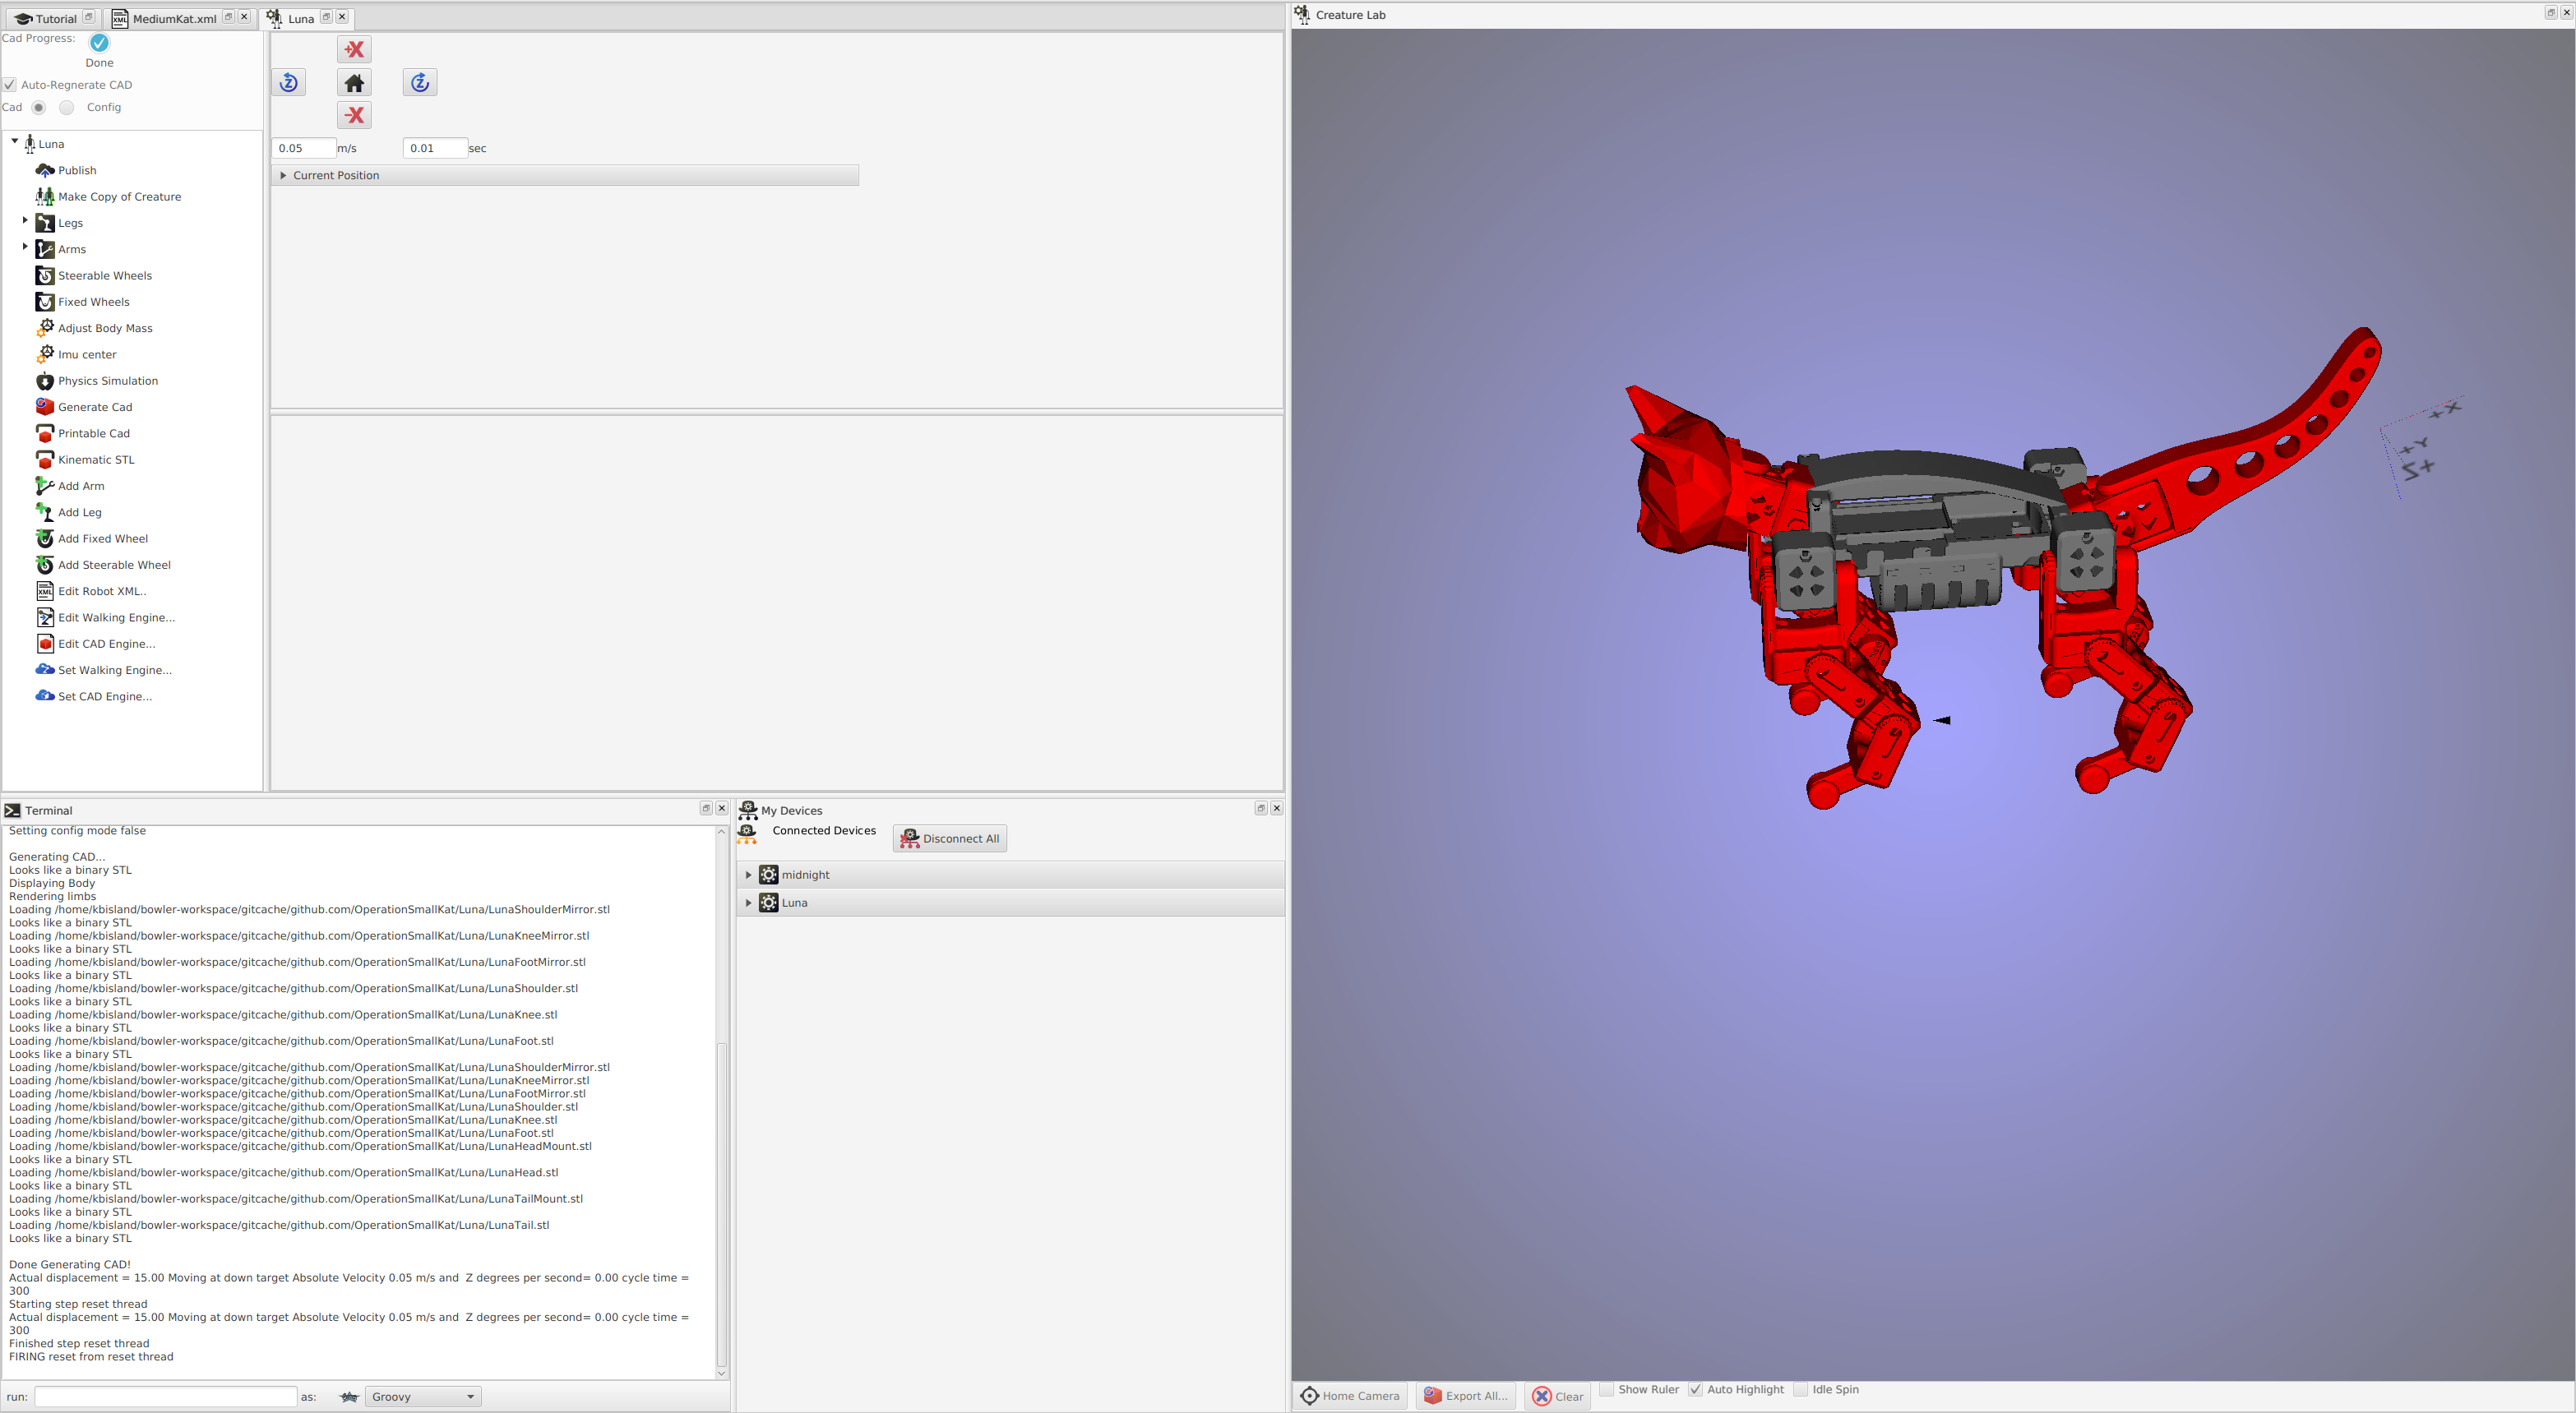
\includegraphics[width=0.9\textwidth]{Images/bowler.png}
    \caption{SmallKat implemented in Bowler Studio}
    \label{fig:Bowler}
\end{figure}

%%%%%%%%%%%%%%%%%%%%%%%%%%%%%%%%%%%%%%%%%%%%%%%%%%%%%%%%%%%%%%%%%%%%%%%%%%%%%%%%%%%%%%%%%%%%%%%%%%%%%%%%%

\chapter{4-DOF Development}\label{chap:4Dof}
An concept for the platform was to add a redundant 4$^{th}$ DOF to the lowest extremity of the robot. This would allow for the computation of an orientation to optimize the torque through the limb.This will allow for a more torque and therefore power efficient system as well as allowing the robot to have a further reach in each step and should allow for a more dynamically capable system. With this addition comes a far more complex series of kinematic and dynamic equations.

The addition of this redundant joint, a series of focus points must be analyzed. Primarily, whether or not the minimum torque can be correctly optimized; secondly, the computation time taken to compute the optimized joint angles and the associated gait and finally how can these computations be accelerated to ensure the time deadline can be met reliably. These points are elaborated further in Sections \ref{sec:Toptimization}, \ref{sec:CompTime} and \ref{sec:Coptimization} respectively. All further steps will be performed in simulation using the model developed for the MQP variant of the robot seen in Fig.\ref{fig:MQPKat}.

\begin{table}[H]
\center
\begin{tabular}{|c|c|c|c|c|}
\hline
 i&  $a_i$&  $\alpha_i$&  $d_i$& $\theta_i$ \\
\hline
 1&  0&  0 &  0& $\theta_1 $  \\
 2&  92&  $-\frac{\pi}{2}$ &  0& $\theta_2$ \\
 3&  75&  0&  0& $\theta_3$ \\
 4&  71&  0&  0& $\theta_4$\\
\hline
\end{tabular}
\caption{D-H Parameters 4DOF Leg Configuration}
\label{tab:dh-table-4DOF}
\end{table}


\section{Torque Optimization}\label{sec:Toptimization}
In order to compute the torque in the limb, the forward torque jacobian is used, the derived equations can be seen in Eq.\ref{eq:4DOF_Torque} where $\uptau_i$ represents the torque at each joint, $a_i, d_i, \theta_i and \alpha_i$ reference the respective variables withing the DH parameter Table \ref{tab:dh-table-4DOF}. In order to compute the joint angles $\theta_i$ the inverse kinematics seen in Eq.\ref{eq:4DOF_Kinematics}. This takes in the X, Y and Z for the Target as well as an orientation angle.
\begin{equ}[H]
\begin{minipage}[H]{0.5\textwidth}
\begin{align*}\label{eq:4DOF_Kinematics}
r_1 
&= \sqrt{x^2 +y^2}\nonumber\\
r_2 
&= \sqrt{x^2 +y^2 + z^2}\nonumber\\
r_3 
&= \sqrt{x^2 +z^2}\nonumber\\
\end{align*}
\end{minipage}
\begin{minipage}[H]{0.5\textwidth}
\vspace{-1cm}
\begin{align*}
P_x 
&= r_1 - S(Q)*L4_d\nonumber\\
P_y
&= z - C(Q)*L4_d
\end{align*}
\end{minipage}
\vspace{-2cm}
\begin{align}
\theta_1 
&= \atantwo ( y, x)\\
\theta_{2} 
&= \theta_1 - \cos^{-1}(((L  2_d^2 + L3_d^2) - (P_x^2+P_y^2))/(2*L2_d*L3_d))\nonumber\hspace{0.25cm}\\
\theta_{3} 
&= \cos^{-1}(((P_x^2 +P_y^2)-(L2_d^2 + L3_d^2))/(2*L2_d*L3_d))\nonumber\\
\theta_{4} 
&= -\theta_{2} + \theta_{3}+Q - \pi\nonumber
\end{align}
\myequations{Kinematic Equations for the 4DOF leg configuration}
% \vspace{-1cm}
\caption{Equation \ref{eq:4DOF_Kinematics}: Kinematic Equations for the 4DOF leg configuration}
\end{equ}

\begin{equ}[H]
\begin{align}\label{eq:4DOF_Torque}%'
    \mathbf{\uptau_1} 
    &= F_1*C(\theta_1)*(a_1 + a_3*C(\theta_2 + \theta_3) + a_2*C(\theta_2) + a_4*C(\theta_2 + \theta_3 + \theta_4))\nonumber\\ 
    &+ F_2*S(\theta_1)*(a_1 + a_3*C(\theta_2 + \theta_3) + a_2*C(\theta_2) + a_4*C(\theta_2 + \theta_3 + \theta_4))\nonumber\\
    \vspace{1.5cm}
    \mathbf{\uptau_2 }
    &= F_0*(a_3*C(\theta_2 + \theta_3) + a_2*C(\theta_2) + a_4*C(\theta_2 + \theta_3 + \theta_4))&\nonumber\\ 
    &- F_1*C(\theta_1)*(a_3*S(\theta_2 + \theta_3) + a_2*C(\theta_2) + a_4*S(\theta_2 + \theta_3 + \theta_4))&\nonumber\\
    &+ F_2*C(\theta_1)*(a_3*S(\theta_2 + \theta_3) + a_2*S(\theta_2) + a_4*C(\theta_2 + \theta_3 + \theta_4))&\\
    \vspace{1.5cm}
    \mathbf{\uptau_3} 
    &= F_0*(a_3*C(\theta_2 + \theta_3) + a_4*C(\theta_2 + \theta_3 + \theta_4)) + F_2*C(\theta_1)*(a_3*S(\theta_2 + \theta_3) \nonumber\\
    &+ a_4*S(\theta_2 + \theta_3 + \theta_4)) - F_1*S(\theta_1)*(a_3*S(\theta_2 + \theta_3) + a_4*S(\theta_2 + \theta_3 + \theta_4))\nonumber\\
    \vspace{1.5cm}
    \mathbf{\uptau_4} 
    &= a_4*F_0*C(\theta_2 + \theta_3 + \theta_4) + a_4*F_2*S(\theta_2 + \theta_3 + \theta_4)*C(\theta_1)\nonumber\\
    &- a_4*F_1*S(\theta_2 + \theta_3 + \theta_4)*S(\theta_1)\nonumber
\end{align}
\myequations{Torque Jacobian of the 4DOF leg configuration}
% \vspace{-1.25cm}
\caption{Equation \ref{eq:4DOF_Torque}: Torque Jacobian of the 4DOF leg configuration}
\end{equ}

To compute the optimal torque an iterative solver was implemented. The target position in X, Y and Z is kept consistent, the end effector orientation angle is then incremented starting at the final joint minimum angle through to the maximum reachable angle. The inverse kinematics at each of these positions and orientations is computed and the joint angles passed to the torque jacobian solver. This result is then stored and analyzed to find the minimal torque value and orientation angle associated with it. This is then passed to the simulation environment and executed on the robot. This iterative solver is very slow and can be optimized in a number of ways, however it was used to confirm the theory is valid.

\section{Computation Time}\label{sec:CompTime}
Due to the number of computation cycles required to compute the optimal orientation angle needed a number of precursory steps were taken including choosing a predetermined orientation angle and computing the gait using that, pre-computing the optimal angle in the case of a static gait and continuously optimizing the orientation angle for all limbs at every stage of a dynamic walking gait. These were performed in this order to prove the potential functionality of each approach as the failure to successfully execute the gait a given manner would result in the next being infeasible.

\subsection{Preset Orientation}

In testing, to ensure the robot was capable of walking and in ensuring all kinematic equations are being computed correctly, the orientation angle was computed manually to ensure a good placement to ensure stability. This angle addition required nearly no additional computational time as it would be executed as a simple inverse kinematic computation. The use of a fixed orientation proved all equations and interfaces were working as expected and were able to be computed in withing the required 2ms time frame. The computation time using this method varied very minimally to tat required for the 3 DOF system, however the torque was not optimized and in end resulted in a higher overall current required by the system due to the increased weight and the addition of the extra motor.

\subsection{Computed Static Optimal Orientation}
Due to the nature of a static walking gait where every step is identical, the optimal orientation for every point within the trajectory can be pre computed. This requires the computationally intensive computation to be done once at the beginning of the testing on the robot. This can then be used to compute all further inverse kinematic calculations. After this is done the computation follows identically to that one in the preset orientation. In end this approach would only work to satisfy a static walking gait with no external input or uneven terrain, generally defeating the purpose of a quadruped robot.  


\subsection{Computed Dynamic Optimal Orientation}\label{sec:DynamicOptimization}
In order to fully utilize the platform and effectively use the full potential of the redundant 4$^{th}$ DOF, a dynamic gait should be utilized. This gait would take into account all external forces applied to the robot and its limbs. In order to effectively use the addition, the optimal orientation angle and subsequent inverse kinematics for each limb would have to be computed at every section through out the gait trajectory computation. This results in a much higher computational load when compared to any other approach used up until this. Using the iterative solver, this would constantly exceed the time provided for this computation and would not be able to be used in this manner. Further devlopemnt would have to be done into accelerating the time taken to complete this computation. This can be seen further in Section \ref{sec:Coptimization}


\section{Computation Optimization}\label{sec:Coptimization}
Given the tight time tolerances required for a dynamic walking gait, the robot buts the able to accurately complete all computations in less than 2ms. If not done the planner will re-begin computation for that partition of the step cycle. Using the techniques set forth in Section \ref{sec:DynamicOptimization} \& \ref{sec:Toptimization}, this 2ms time frame was unable to be met and therefore some adaptations must be made to complete the computations in the given time.
\subsection{Assumptions}\label{sec:assumptions}
In order to accelerate the time taken to compute the optimal orientation angle and the subsequent inverse kinematics in a 2ms time frame, a number of assumptions must be made. Primarily, the assumption that the limb torque would follow a trend similar to that of an inverted Gaussian curve an example of which is seen in Fig. \ref{fig:AssumedTorque}. This torque cure demonstrated that the optimal orientation angle exists at the point of lowest torque. Secondly, it was assumed that there would be only one global minima to the torque curve meaning there would be only one optimal orientation angle. 


\begin{figure}[H]
    \centering
    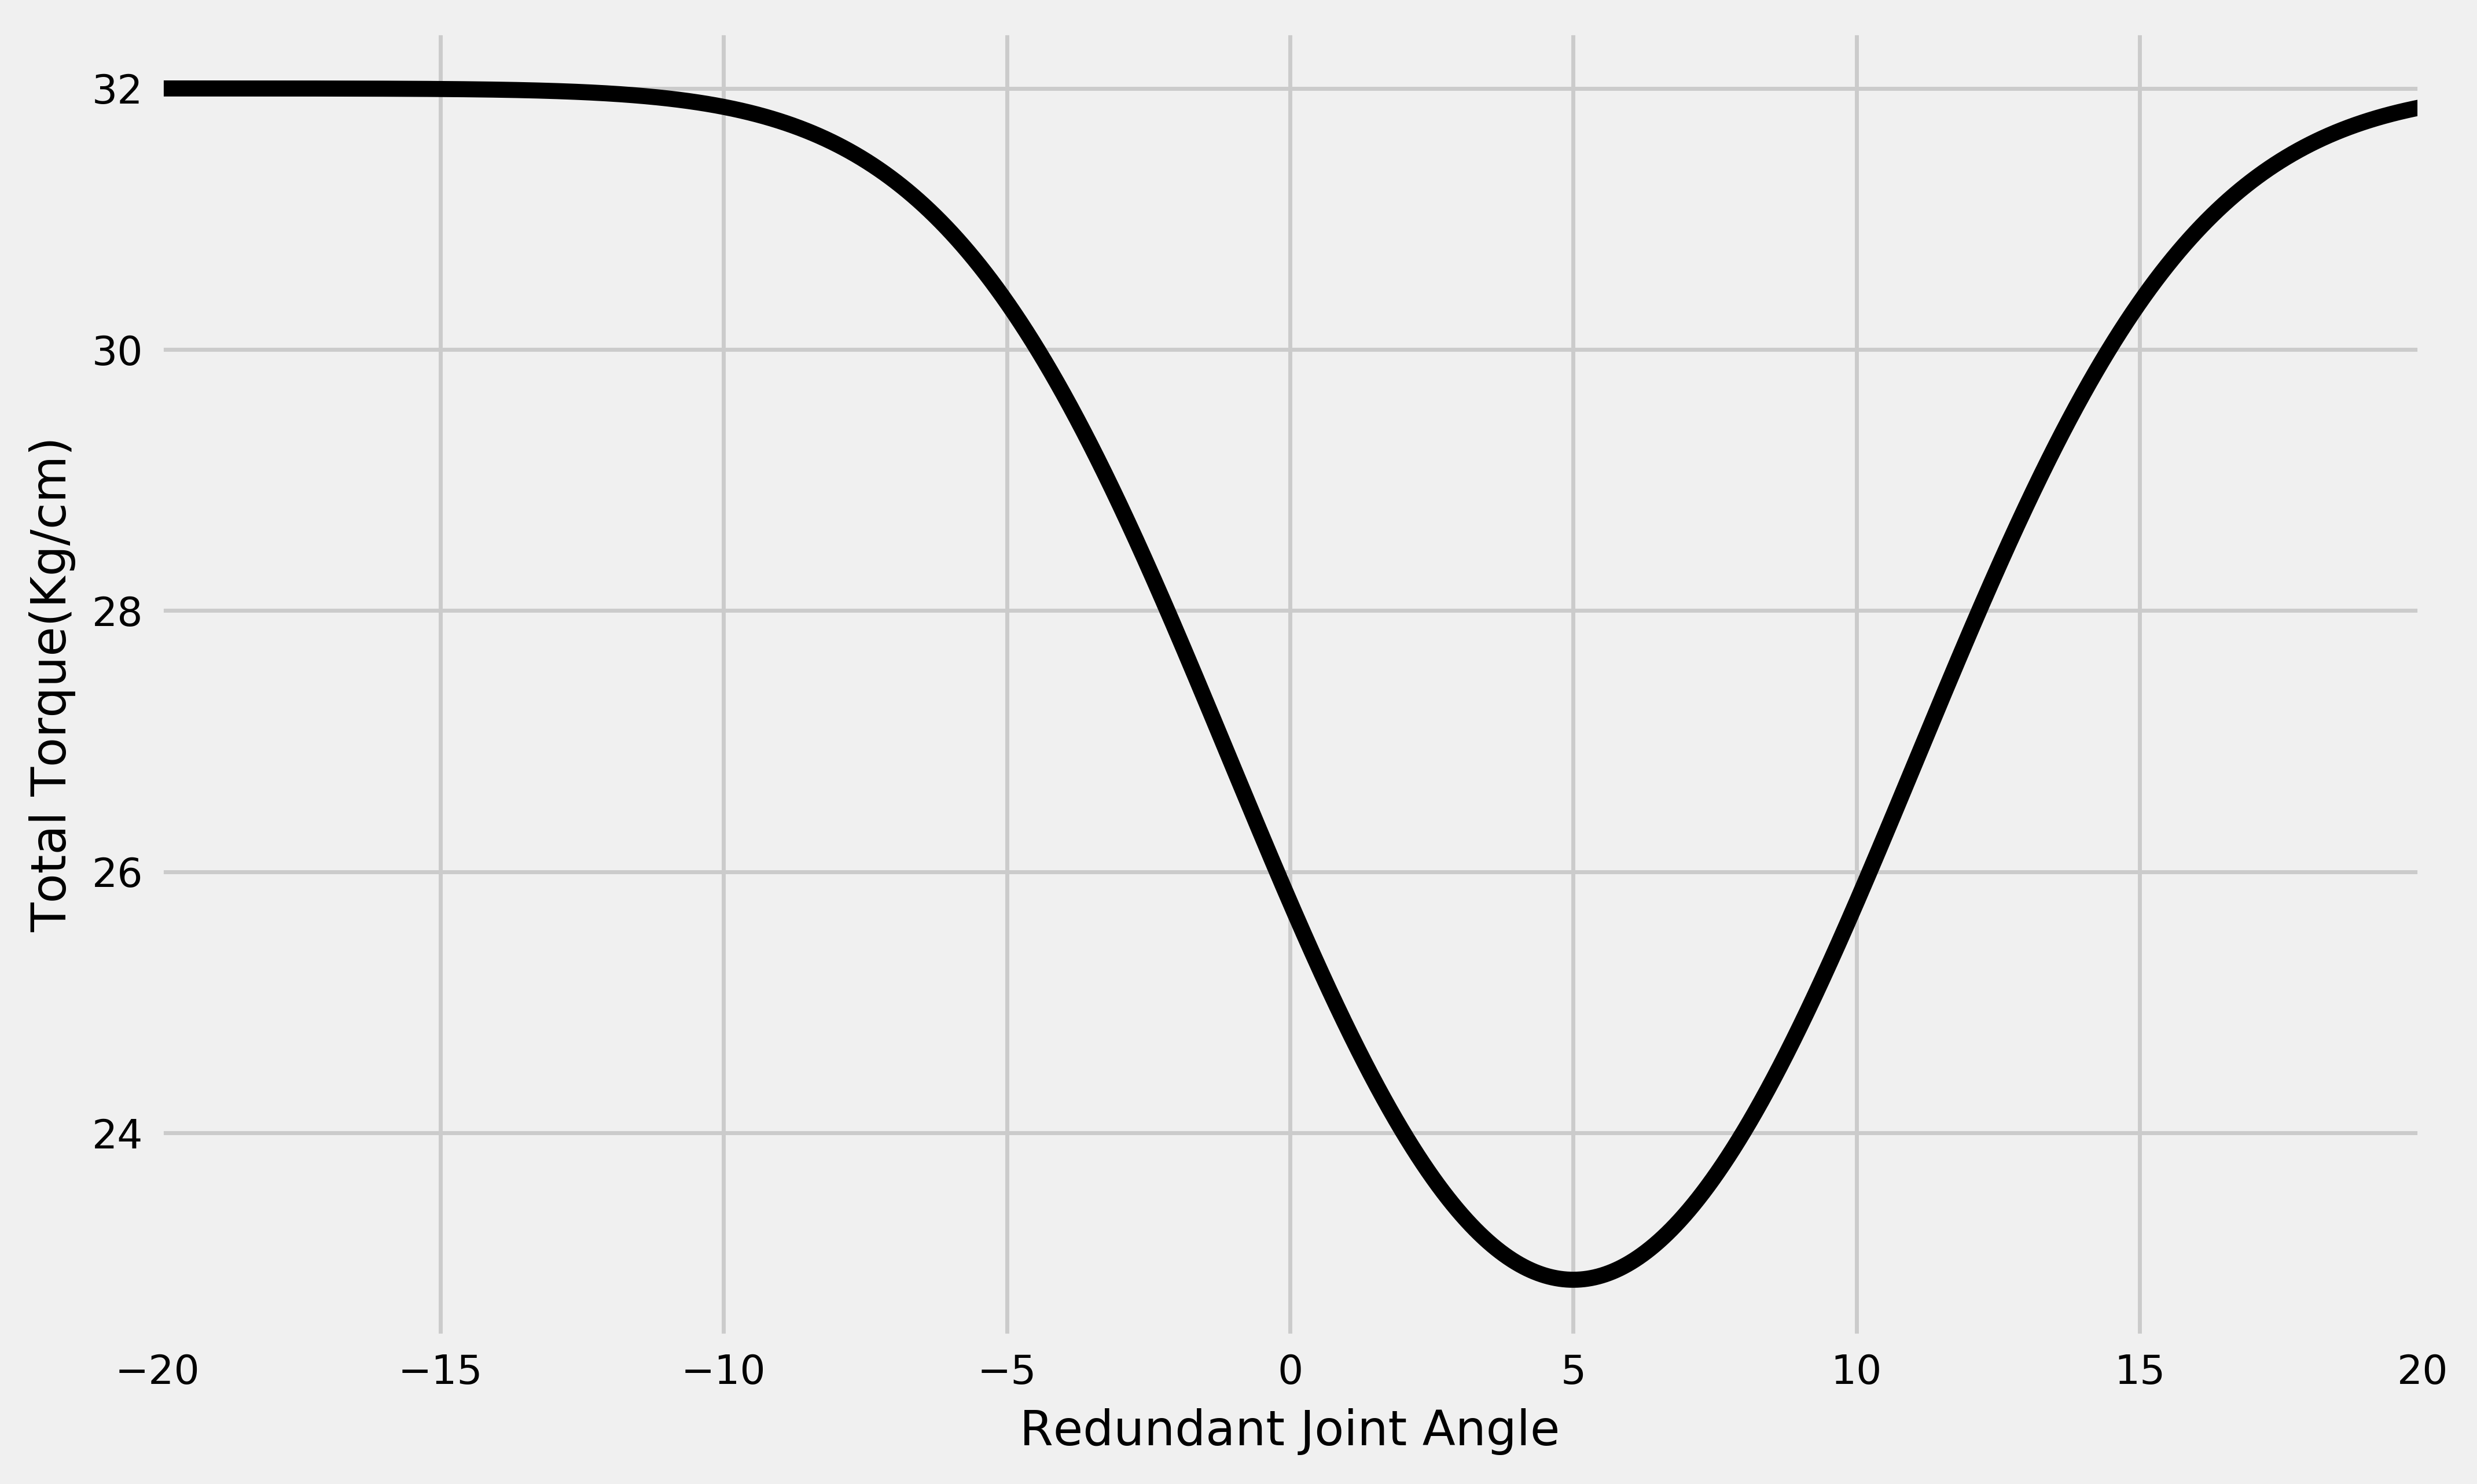
\includegraphics[width=0.6\textwidth]{Images/torqueCurve.png}
    \caption{Assumed torque profile of a limb with reference to orientation angle}
    \label{fig:AssumedTorque}
\end{figure}
\subsection{Computation Time Acceleration}
In an attempt to validate whether the addition of the 4$^{th}$ DOF was feasible with the existing software computation structure, a rudimentary computation acceleration algorithm was developed. This algorithm approximates the optimal orientation angle by starting two computational threads running in parallel. Each thread will compute the torque propagated through the system in 5$^{\circ}$ increments from a given starting pose being the upper and lower extreme of the final joints range of motion. 

Each iteration, the inverse kinematics are computed and the joint angles are passed to the forward torque jacobian solver and the joint torque is recorded. The next iteration is then computed and the torque compared to the previous iteration. Following the assumptions established in Section \ref{sec:assumptions}, the proximal iteration should have a lower torque total if it is tending towards the optimal orientation angle. This is continued until both threads have surpassed the global minima by having a torque increase instead of decrease. The process is then repeated in finer 1$^{\circ}$ increments until both threads converge on an optimal value. This orientation angle is then used, the Inverse kinematics are computed and passed to the simulation environment and executed on the robot. 

This computational acceleration resulted in an overall decrease in the amount of time taken to compute the optimal orientation angle, however it did not reduce it enough to reliably compute all necessary computations in the time dedicated to gait computation. This resulted in this ending the research being done into this addition on the system. Further optimization involved in the calculation of an optimal torque by this method or by other more advanced methods may make the addition of the redundant 4$^{th}$ DOF feasible, however it was outside of the scope of this thesis project. 
%%%%%%%%%%%%%%%%%%%%%%%%%%%%%%%%%%%%%%%%%%%%%%%%%%%%%%%%%%%%%%%%%%%%%%%%%%%%%%%%%%%%%%%%%%%%%%%%%%%%%%%%%

\chapter{Implementation}
\section{Course Implementation}
    To test the robots hardware abilities as well as the software developed for the platform both at a high and low level, a course was developed with course material as well as lab material and was implemented as a voluntary ISP with 3 students. Each week these students were given a series of videos and lecture slides that cover the topics for the week ranging from an introduction to kinematics through trajectory planning and gait generation.  Along with this each week the students were assigned tasks to complete as lab material, each student worked independently on the project with support and advise from the SmallKat team and the project advisors. The students followed a course schedule as seen in Table \ref{tab:CourseSchedule}. 
    
\begin{table}[H]
    \centering
        \begin{tabular}{|c|c|c|}
            \hline
            Week & Course Topic & Lab Task\\
            \hline
              1   & \thead{Familiarize with robot and software} & Assemble robot\\            \hline

              2   & \thead{Familiarize with scripting \\interface} & \thead{Test robot with \\test software}\\            \hline

              3   & \thead{How to create a\\ walking cycle} & \thead{Perform static motion, \\movement in Z}\\            \hline

              4   & \thead{How to create a\\ walking gait trajectory}  & \thead{Develop and test \\trajectory on one leg}\\            \hline

              5   & \thead{Balancing based \\on contact area} & \thead{Adjust the pose of the \\robot based on IMU input}\\            \hline

              6   & \thead{Trajectory planning \\and threads} & \thead{Integrate threading into \\the trajectory generation}\\            \hline

              7   &  & \thead{Final Evaluation, \\walking and turning}\\
              \hline
        \end{tabular}
    \caption{SmallKat ISP Course Schedule}
    \label{tab:CourseSchedule}
\end{table}

All student concerns were recorded and addressed through out the course. These ranged from assembly instruction modifications to integration and addition of more sensors for future advancement and development. At the end of the course the students were asked for feedback on the platform as a whole with an overall positive response with minor changes for improvements. Since then, all concerns that would not change the robots price point drastically have been integrated into a revision of the robot including a revised power management system and updated robot firmware and a number of mechanical advancements. 

As a final project for the course, each student was tasked to develop a walking gait for the robot  with the ability to walk straight and turn. On completion of this bonus credit would be given for smoothing the walking of the robot by integrating the head and tail for a dynamic inertial shift to help to keep the robot level. Further credit would be awarded for the development of a semi dynamic gait which would use the head and tail to balance the robot in the case of an external input such as mildly uneven terrain. All students were able to accomplish the task of developing a successful walking gait with most able to integrate the head and tail for dynamic balancing. After completion, most of the students were interested in further developing on the system and extending this project into future work.
%%%%%%%%%%%%%%%%%%%%%%%%%%%%%%%%%%%%%%%%%%%%%%%%%%%%%%%%%%%%%%%%%%%%%%%%%%%%%%%%%%%%%%%%%%%%%%%%%%%%%%%%
\section{Platform Testing}
    While making changes to so many aspects of the robot a large amount of testing has to be performed to ensure reliability and measurable improvements to the system as a whole. These changes were made in three major divisions: Software, Mechanical and Electrical. each of which will be spoken about in the following sections.
    \subsection{Software testing}
        In order to test the software changes a known working platform was kept whit no hardware changes made to ensure any software changes that were made at either the high level in Bowler Studio as it pertained to communication, gait generation or general usability. These changes were then tested using the reference robot being a Grace model seen in Fig.\ref{fig:Grace} as it was a known good platform utilizing the same gait planner and kinematics engine with changes only being made to the robot specific DH-Parameters. After confirmed working the changes were then tested using the new hardware to ensure it continued to function as expected.
    \subsection{Electrical}
        For the electrical system there are a number of validation steps to ensure full functionality and reliability. Primarily the boards were tested for full functionality, ensuring it was able to correctly provide 16 servo PWM signals and control them independently, it was able to communicate with all onbaord sensors and the main micro controller was able to be programmed successfully with the integrated programming circuit. Secondly the power supply integrated onto the board was tested for resilience, the power supply was set to provide 10A at 6V which would be much higher than the general use case however is a possible current the robot is expected to draw during certain motions; an electronic load was then used to draw full power from the board until failure, the supply was able to continuously provide 10A at 6V stably for over 2 hours at which time the test was stopped and the power supply concluded as acceptable. Finally the new motherboard was tested in a physical robot, utilizing the Grace model seen in Fig.\ref{fig:Grace} to start as it was a known working model and then the Luna model seen in Fig.\ref{fig:Luna}. These tests were done successfully and any issues were fixed in further board revisions.
    \subsection{Mechanical}
        When designing the Luna model seen in Fig. \ref{fig:Luna} a number of precursor tests were done to test the lifting strength of the motors. a test leg was developed and assembled using the chosen servos and tested for its ability to support and estimated weight. Once this was done the dimensions of the leg were adjusted and the remainder of the robot was printed and assembled. After minor adjustments and tolerance updates a finalized model was completed. 
        
        Once a final model was completed, the legs were then printed in a number of materials including PLA, PETG, ABS, Poly-Carbonate and nylon. Each of these have a variety of benefits and disadvantages. Most of these are easily printable and reliable. Each of these legs were assembled and tested for link failure, this would occur due to heat generated by the motor causing the plastic to deform. In end PETG was the chosen material as it comes with a number of temperature performance benefits as well as cost benefits. When using PETG there was no notable deformation after the testing. Many other materials were also able to withstand the temperature change but came with an increased cost or difficulty in printing. 
        
        \begin{table}[H]
            \centering
            \begin{tabular}{|c|c|c|c|}
            \hline
            Material & Glass Transition Temperature ($^{\circ}$C)& Cost (\$/Kg) & Ease of Printing   \\
            \hline
              PLA   & 60 & 22  & High \\ \hline
              ABS     & 105  &  25 & Low\\ \hline
              PETG     & 88 & 25 & High\\ \hline
              PC     & 147 & 53  & Low\\ \hline
              Nylon   & 70 & 45  & Medium\\
              \hline
            \end{tabular}
            \caption{Material Comparison}
            \label{tab:MaterialsTable}
        \end{table}
\chapter{Results}\label{chap:Results}

\begin{figure}
        \centering
        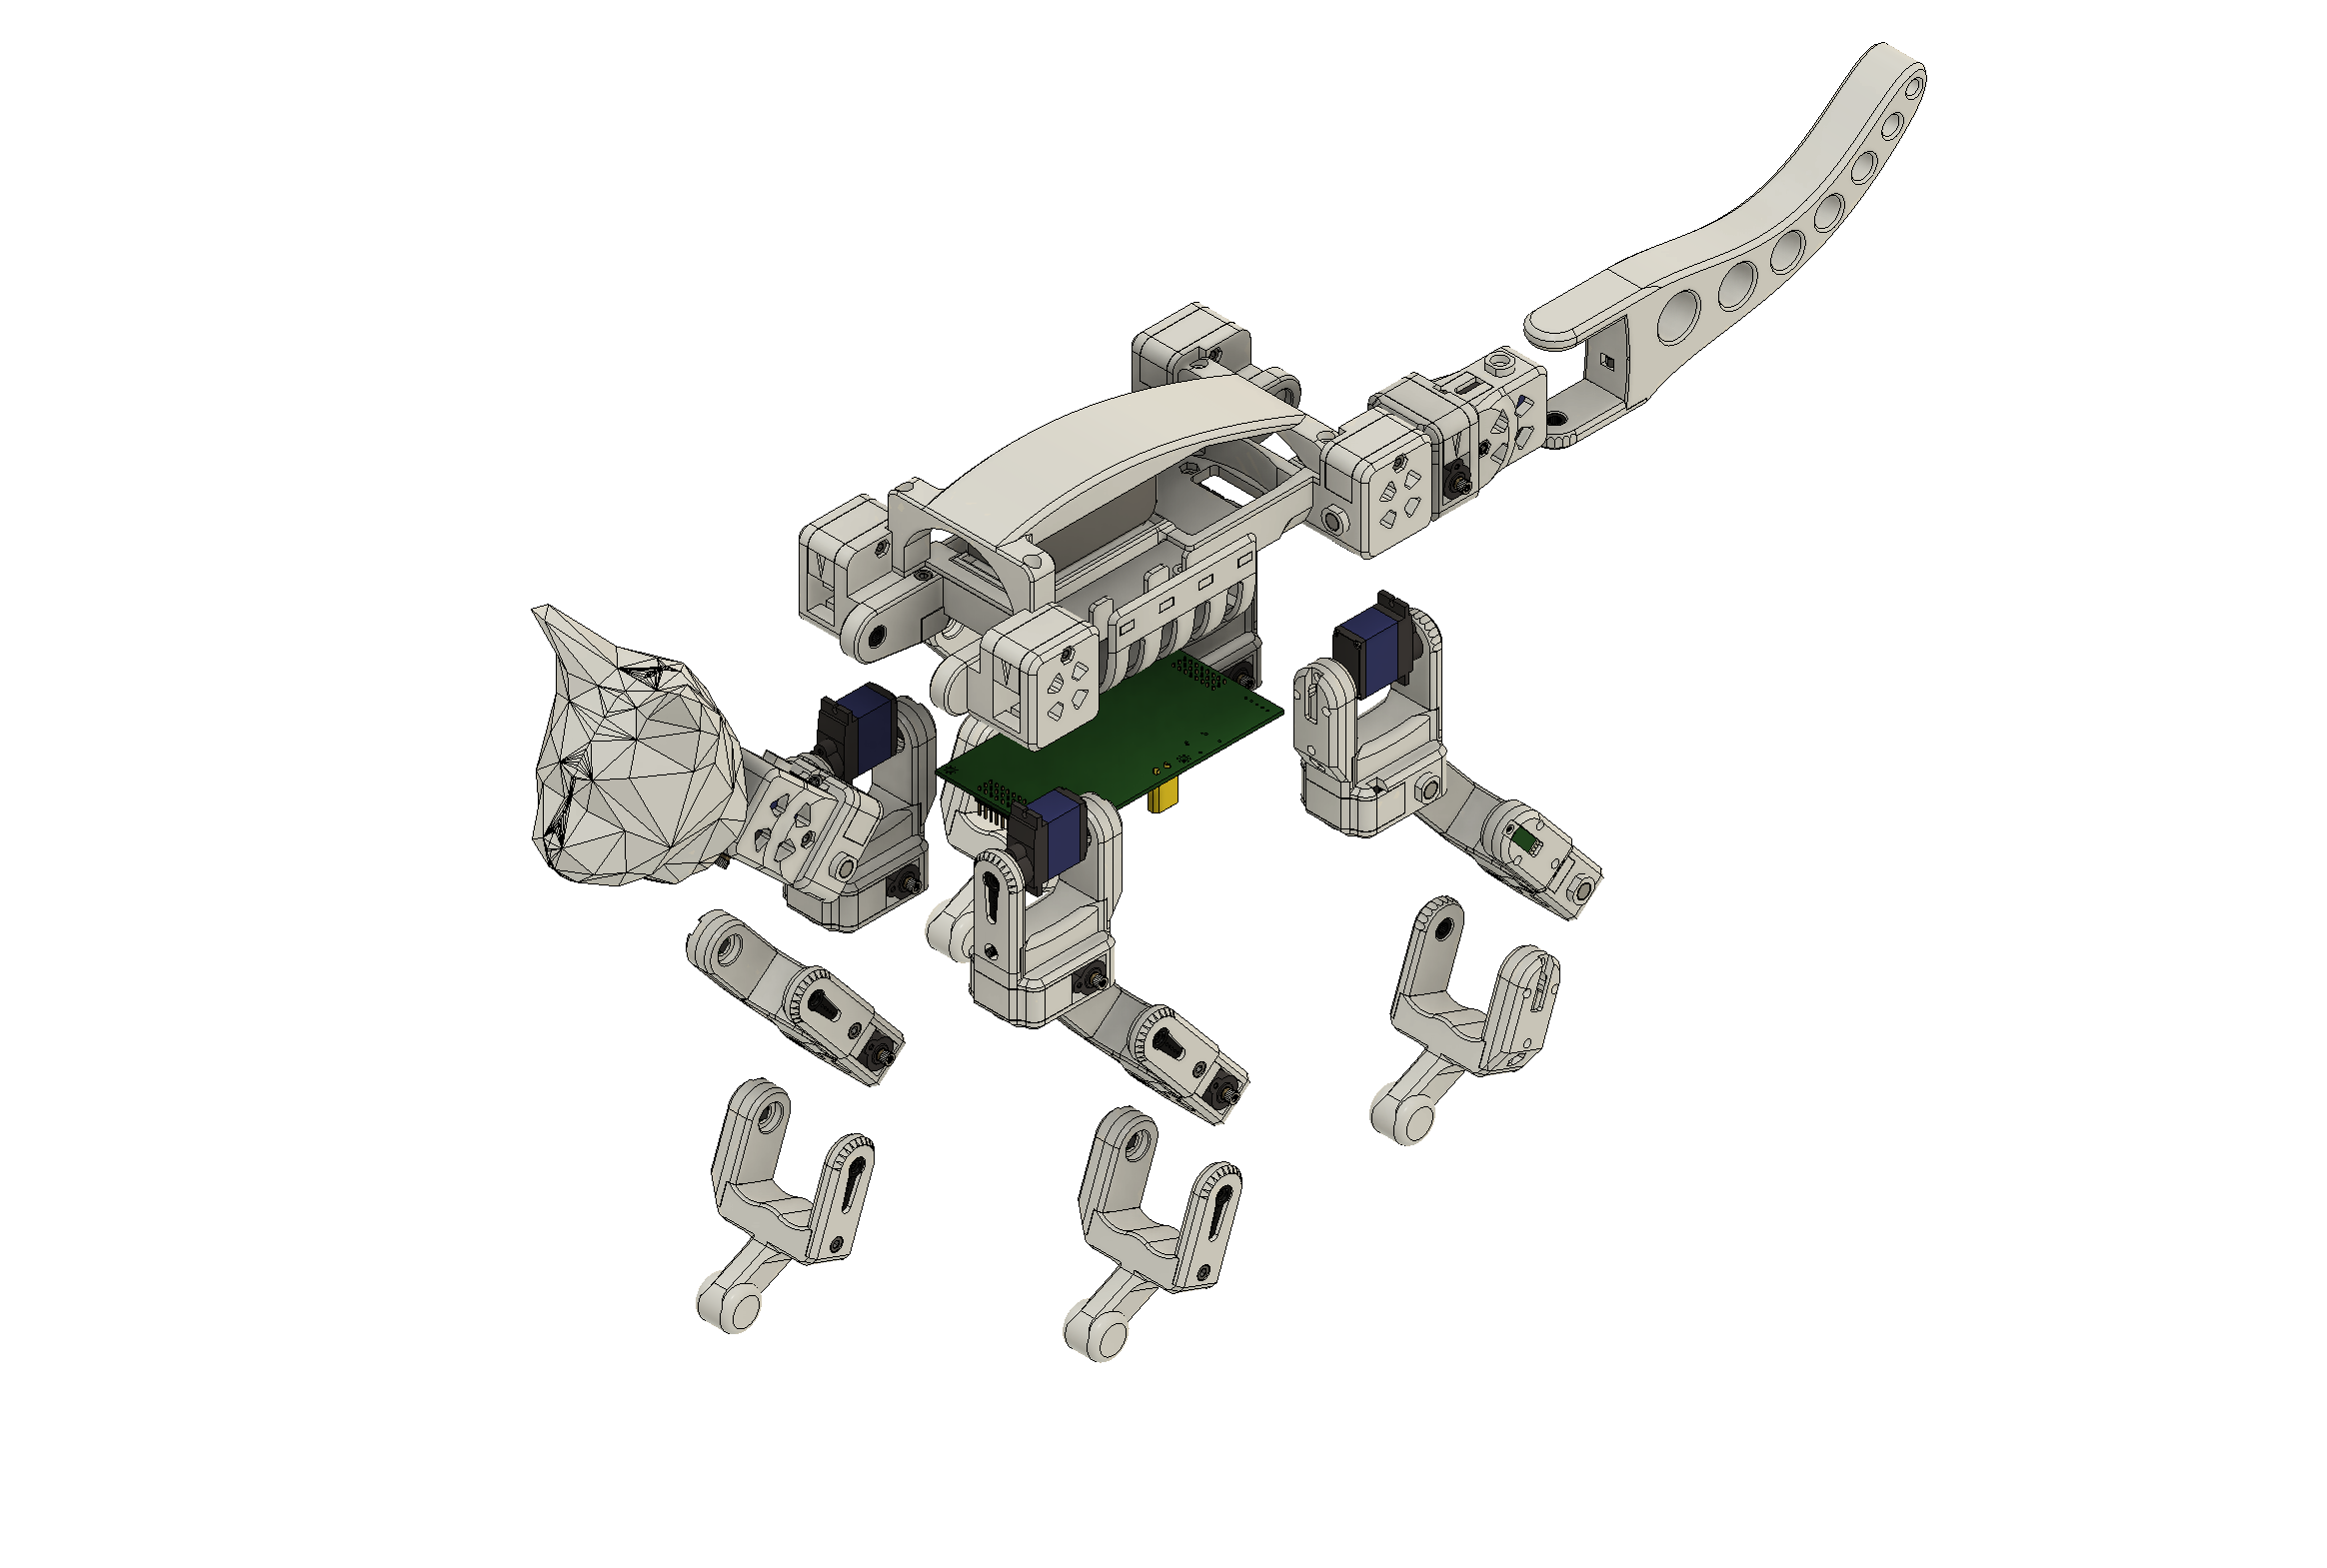
\includegraphics[width = 0.7\textwidth]{Images/ExplodedView.PNG}
        \caption{Exploded View of the Robot}
        \label{fig:ExplodedView}
    \end{figure}
    
\begin{figure}
        \centering
        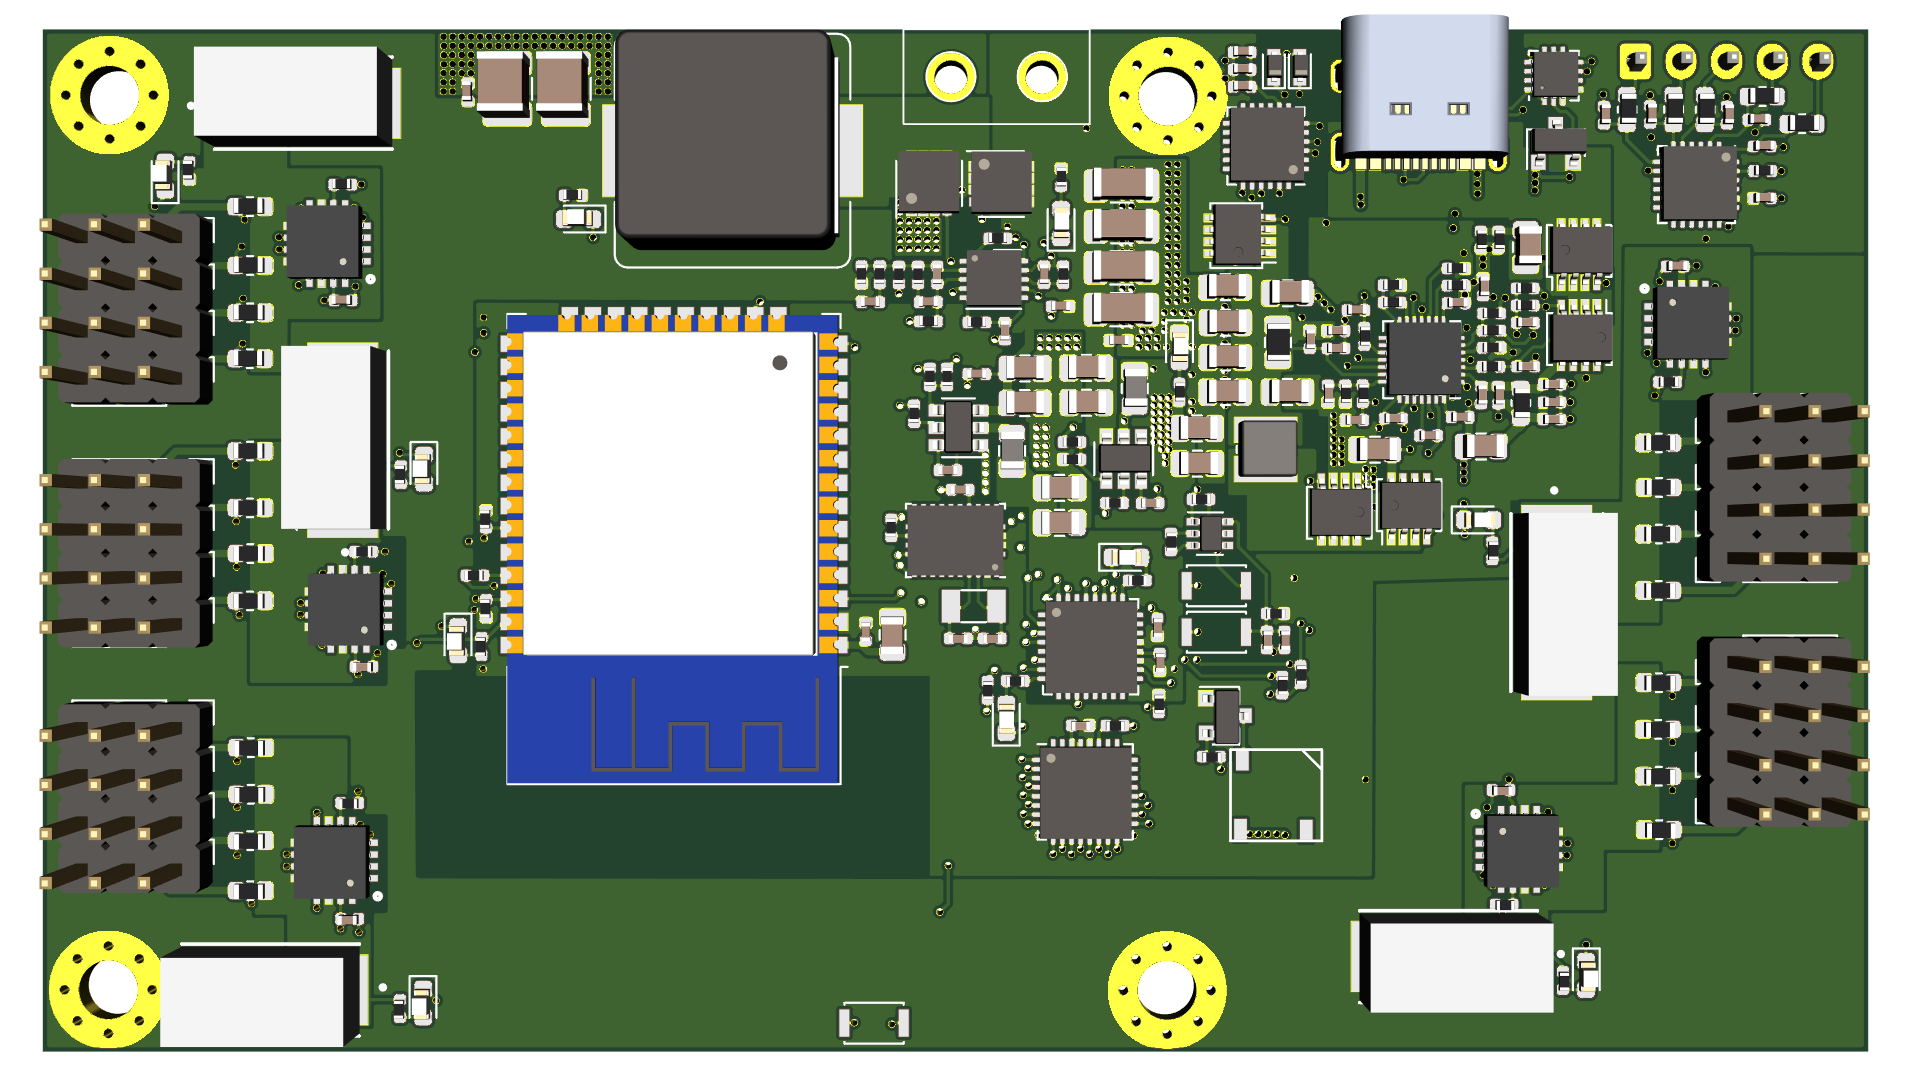
\includegraphics[width = 0.7\textwidth]{Images/Motherboard.png}
        \caption{Exploded View of the Robot}
        \label{fig:ExplodedView}
    \end{figure}
A series of tests were run to compare the robots ability to perform tasks required for the teaching objectives listed in section \ref{sec:DesignReqs}. In order to prove the robots ability to correctly demonstrate forward and inverse kinematics and to ensure the kinematic equations being used were accurate, high accuracy magnetic encoders were attached to the joints and the joint angles recorded through out the actions. In order to prove the inverse kinematic of the system, an initial reachable point in a legs work space was given and a second point in the work space  and the path the leg followed is compared to the theoretical, straight line path between the two points is shown in Fig. \ref{fig:IK}

    \begin{figure}[H]
	\centering
      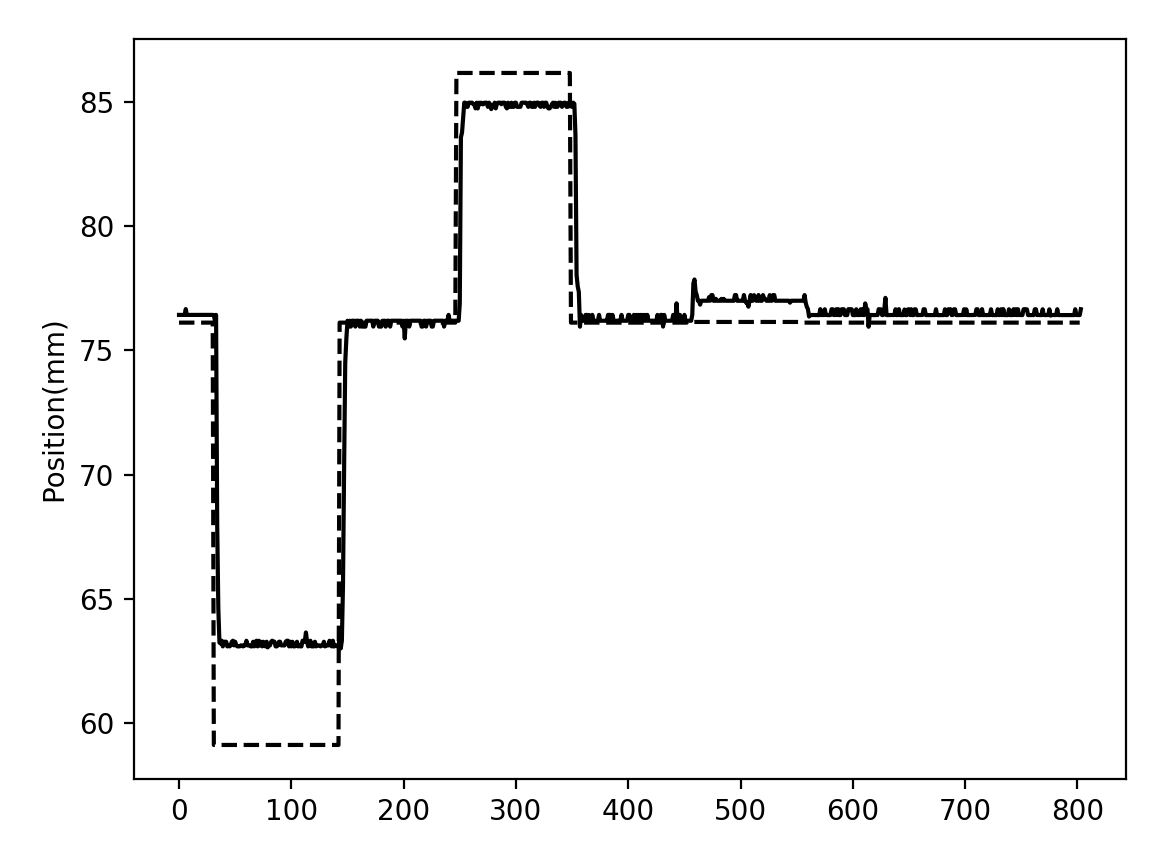
\includegraphics[width=0.6\textwidth, height =4cm]{Images/PosPlotX.png} % I will update to have a legend
      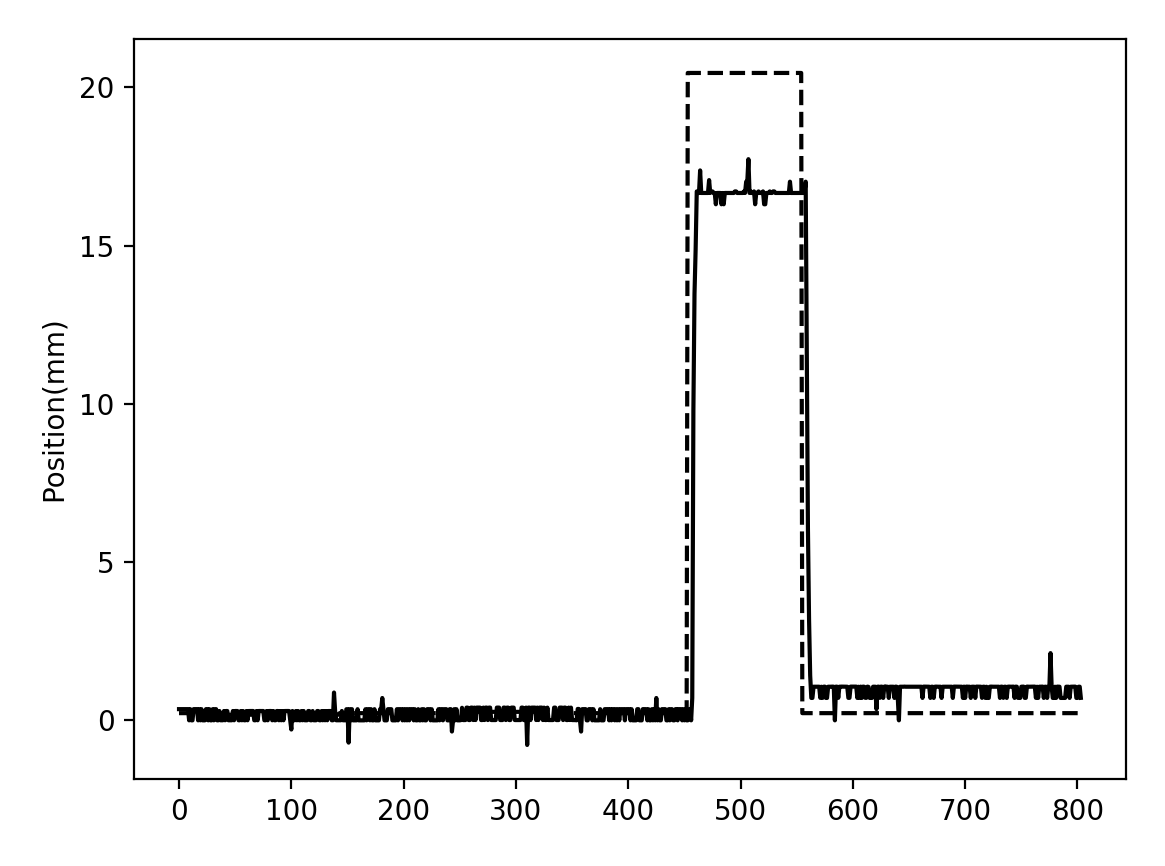
\includegraphics[width=0.6\textwidth, height =4cm]{Images/PosPlotY.png} % I will update to have a legend
      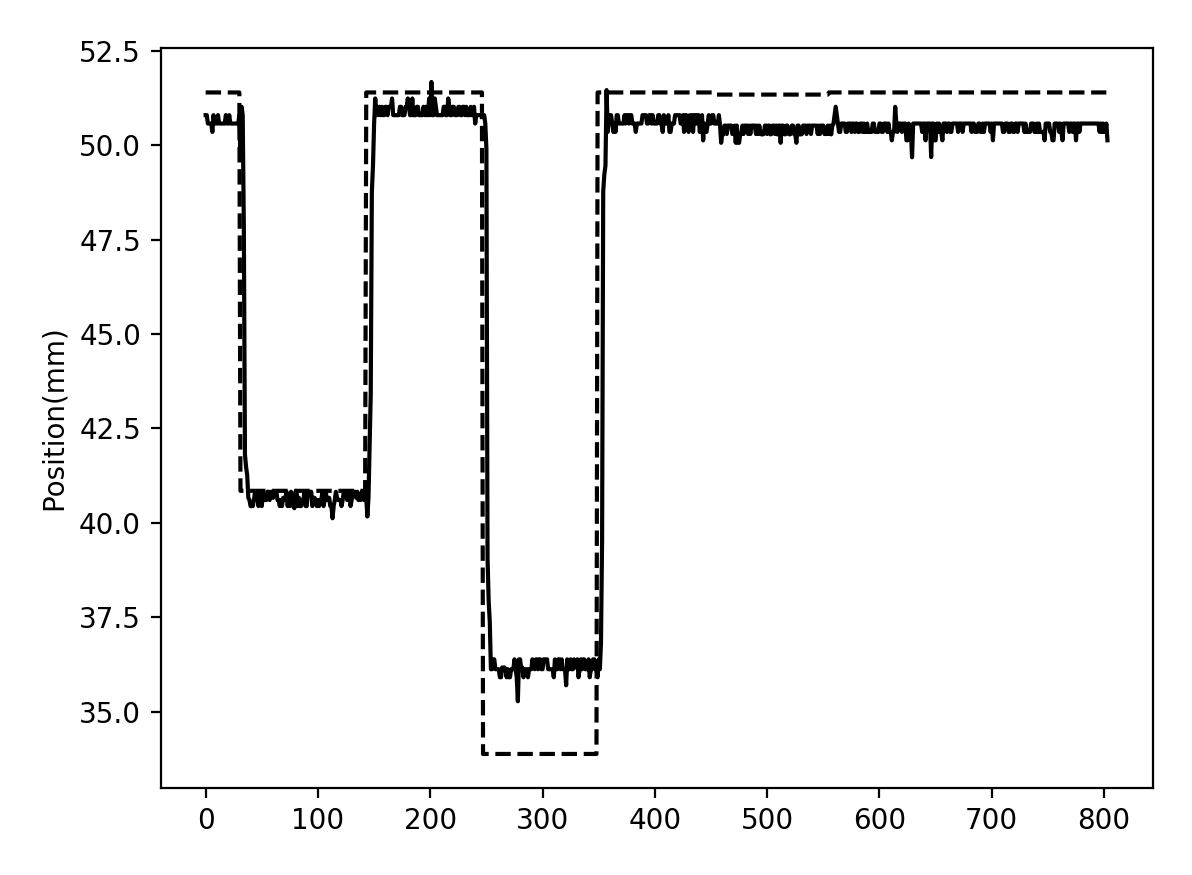
\includegraphics[width=0.6\textwidth, height =4cm]{Images/PosPlotZ.png} % I will update to have a legend
  	\caption{Graph showing the theoretical vs real trajectory in Inverse Kinematics (Setpoint- Broken Line)}
  	\label{fig:IK}
\end{figure}

Following these tests, testing the ability to follow a given trajectory using a single leg. This was done by generating a trapezoidal trajectory path, similar to that used in the gait generation algorithm with way points along the path. These way points were then used to generate trajectories between the points. The trajectories were then broken into segments and passed in to the inverse kinematic equations and passed to the robot. In the same way the joint angles were collected for the inverse kinematics test, the encoders were used to collect the joint information. To prove the robots ability to perform a generated gait was validated by pre computing a static walking gait and passing it to the robot and having it follow each generated trajectory of each leg. The results of this and the robots ability to follow a trajectory can be seen in Fig. \ref{fig:gait}
    \begin{figure}[H]
	\centering
      \hspace{2mm}
      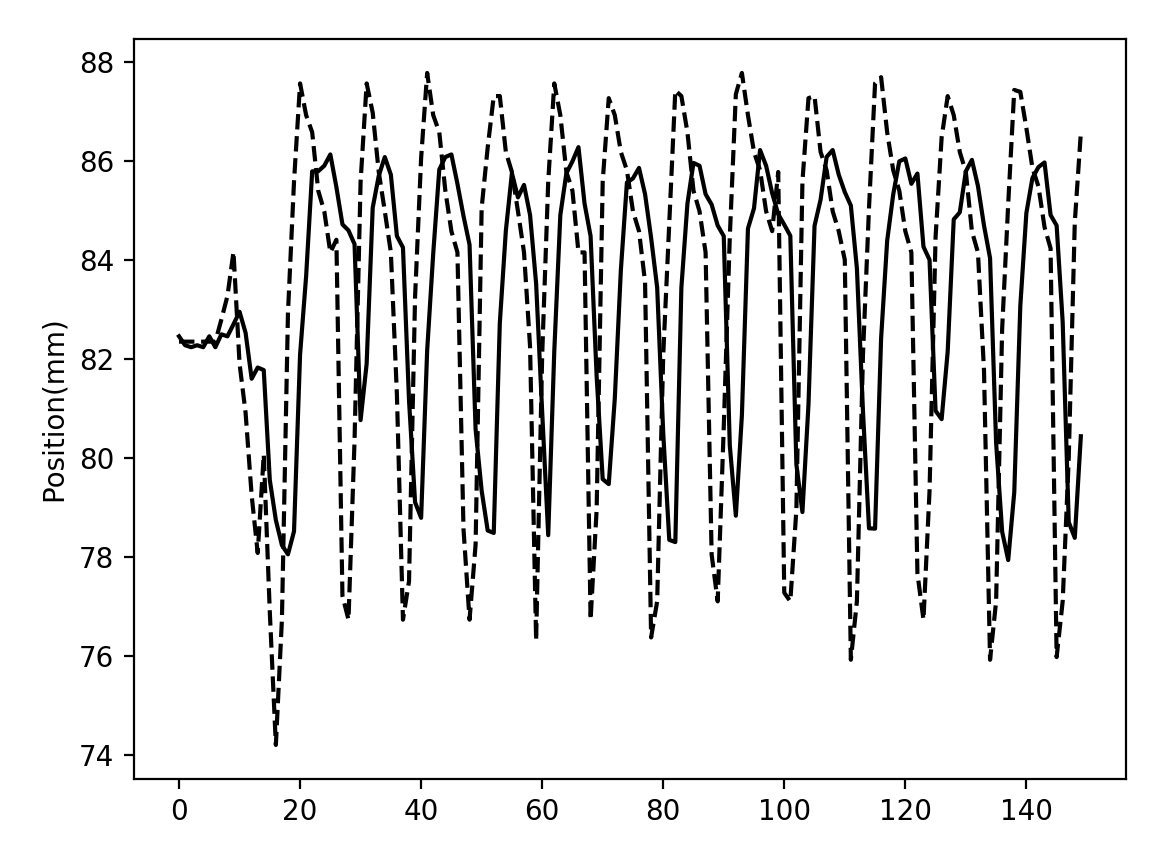
\includegraphics[width=0.6\textwidth, height =4cm]{Images/GaitPlotX.png} % I will update to have a legend
      \hspace{-37mm}%                
      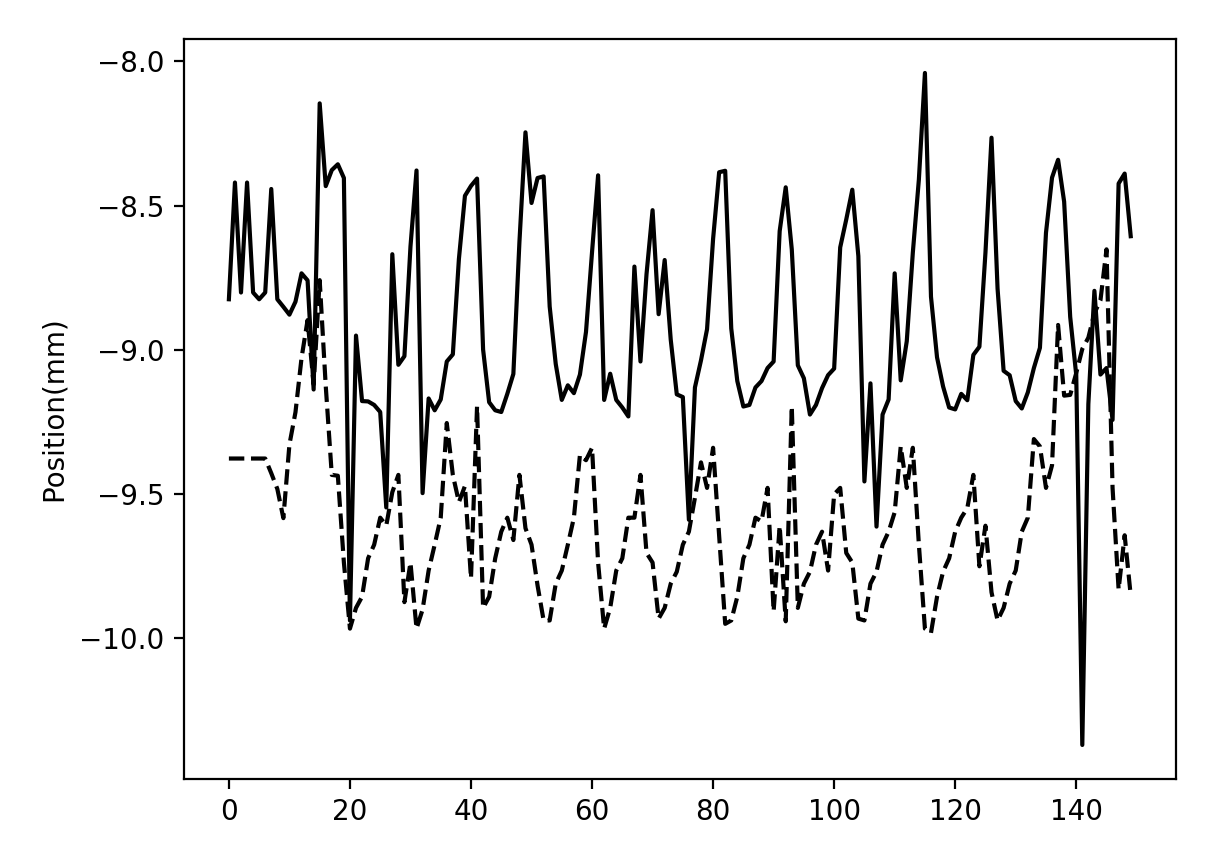
\includegraphics[width=0.64\textwidth, height =4cm]{Images/GaitPlotY.png} % I will update to have a legend
        \hspace{2mm}
      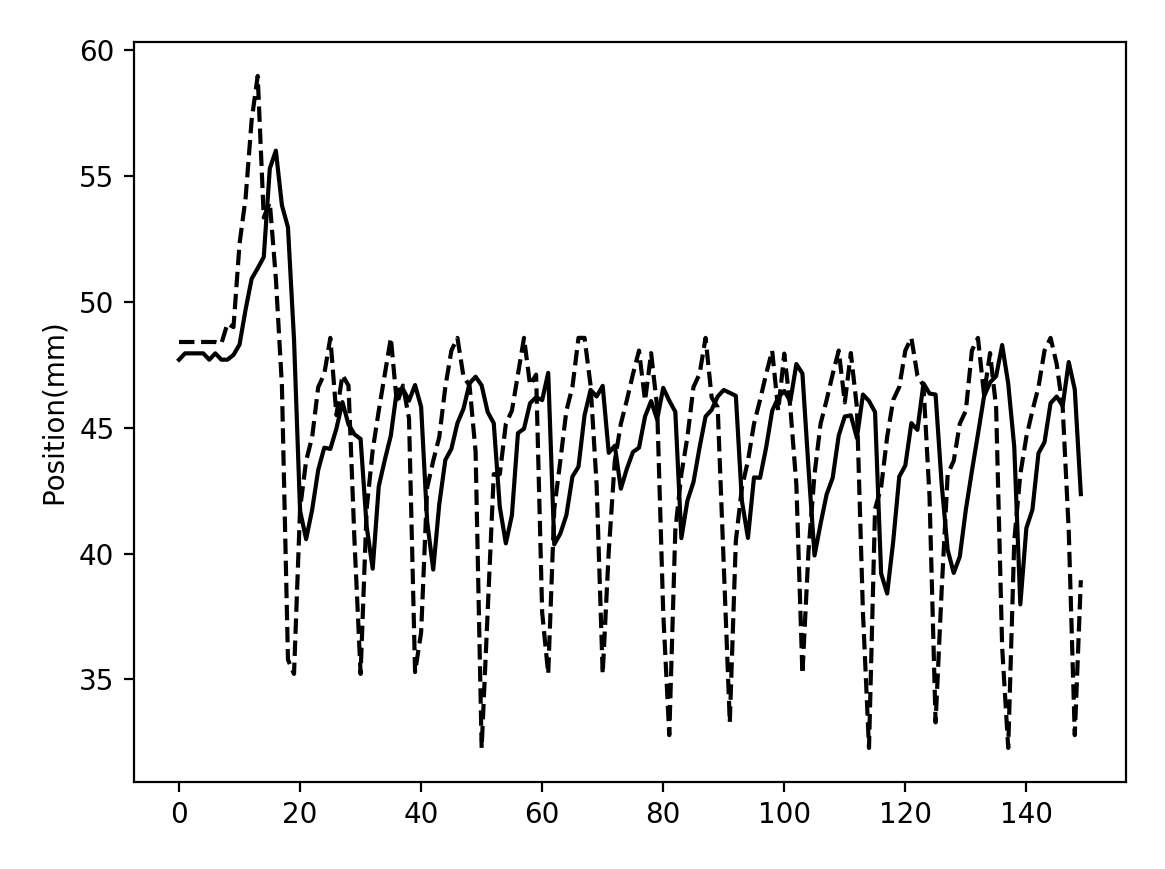
\includegraphics[width=0.6\textwidth, height =4cm]{Images/GaitPlotZ.png} % I will update to have a legend
  	\caption{Graph showing the generated gait vs real gait (Setpoint- Broken Line)}
  	\label{fig:gait}
\end{figure}

As can be seen in Fig.\ref{fig:IK} the robot is able to accurately move between 2 given points and back to the origin, in a controlled motion with a high degree of accuracy with a mean error of 1.72 $\pm$ 2.26mm. This was then tested in the robots ability to follow a generated trajectory, the generated trajectory was a single cycle of the developed walking gait. The robots ability to accurately follow this path is seen in \ref{fig:gait} with a mean error of 1.39$\pm$2.012mm. In the gait cycle developed there is a great margin of error available due to the minor compensation computed by the integrated IMU.

%%%%%%%%%%%%%%%%%%%%%%%%%%%%%%%%%%%%%%%%%%%%%%%%%%%%%%%%%%%%%%%%%%%%%%%%%%%%%%%%%%%%%%%%%%%%%%%%%%%%%%%%%
\begin{figure}[H]
    \centering
    \begin{tikzpicture}[
    pre/.style={=stealth',semithick},
    post/.style={->,shorten >=1pt,>=stealth',semithick}]
    \begin{scope}[xshift=1.5cm]
        \node[anchor=south west,inner sep=0] (image) at (-5.1,0) {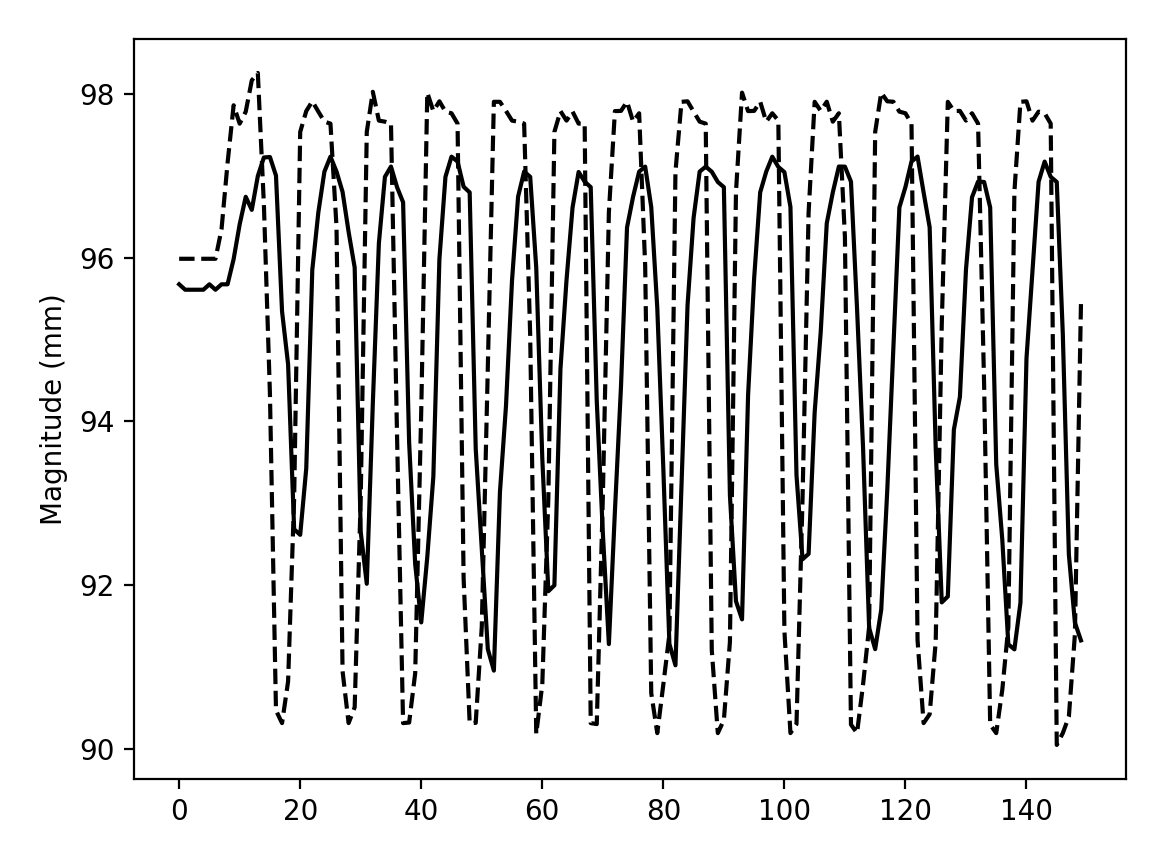
\includegraphics[width=0.6\textwidth, height =4cm]{Images/GaitPlotMagnitude.png}};
         \node[anchor=south west,inner sep=0] (zoomed) at (-2.6,-4.5) {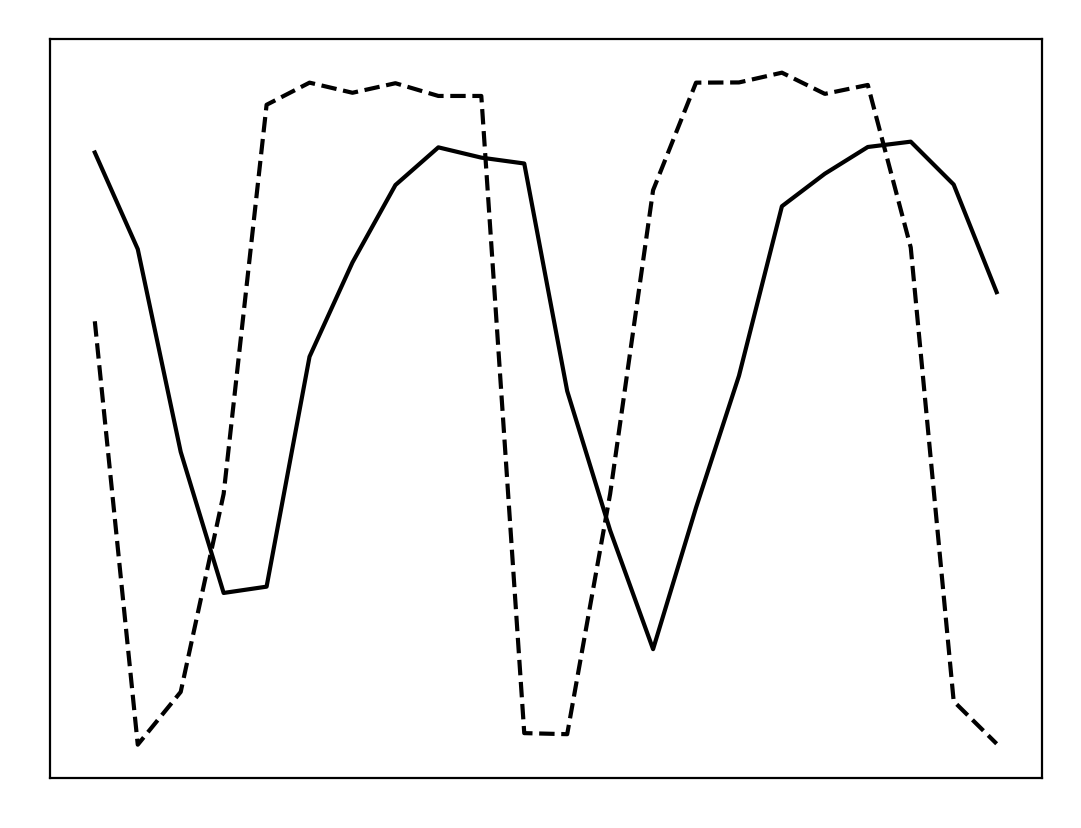
\includegraphics[width=0.3\textwidth]{Images/partialPlotMagnitude.png}};
        \node[anchor=south west,inner sep=0] (im1) at (-8,-8) {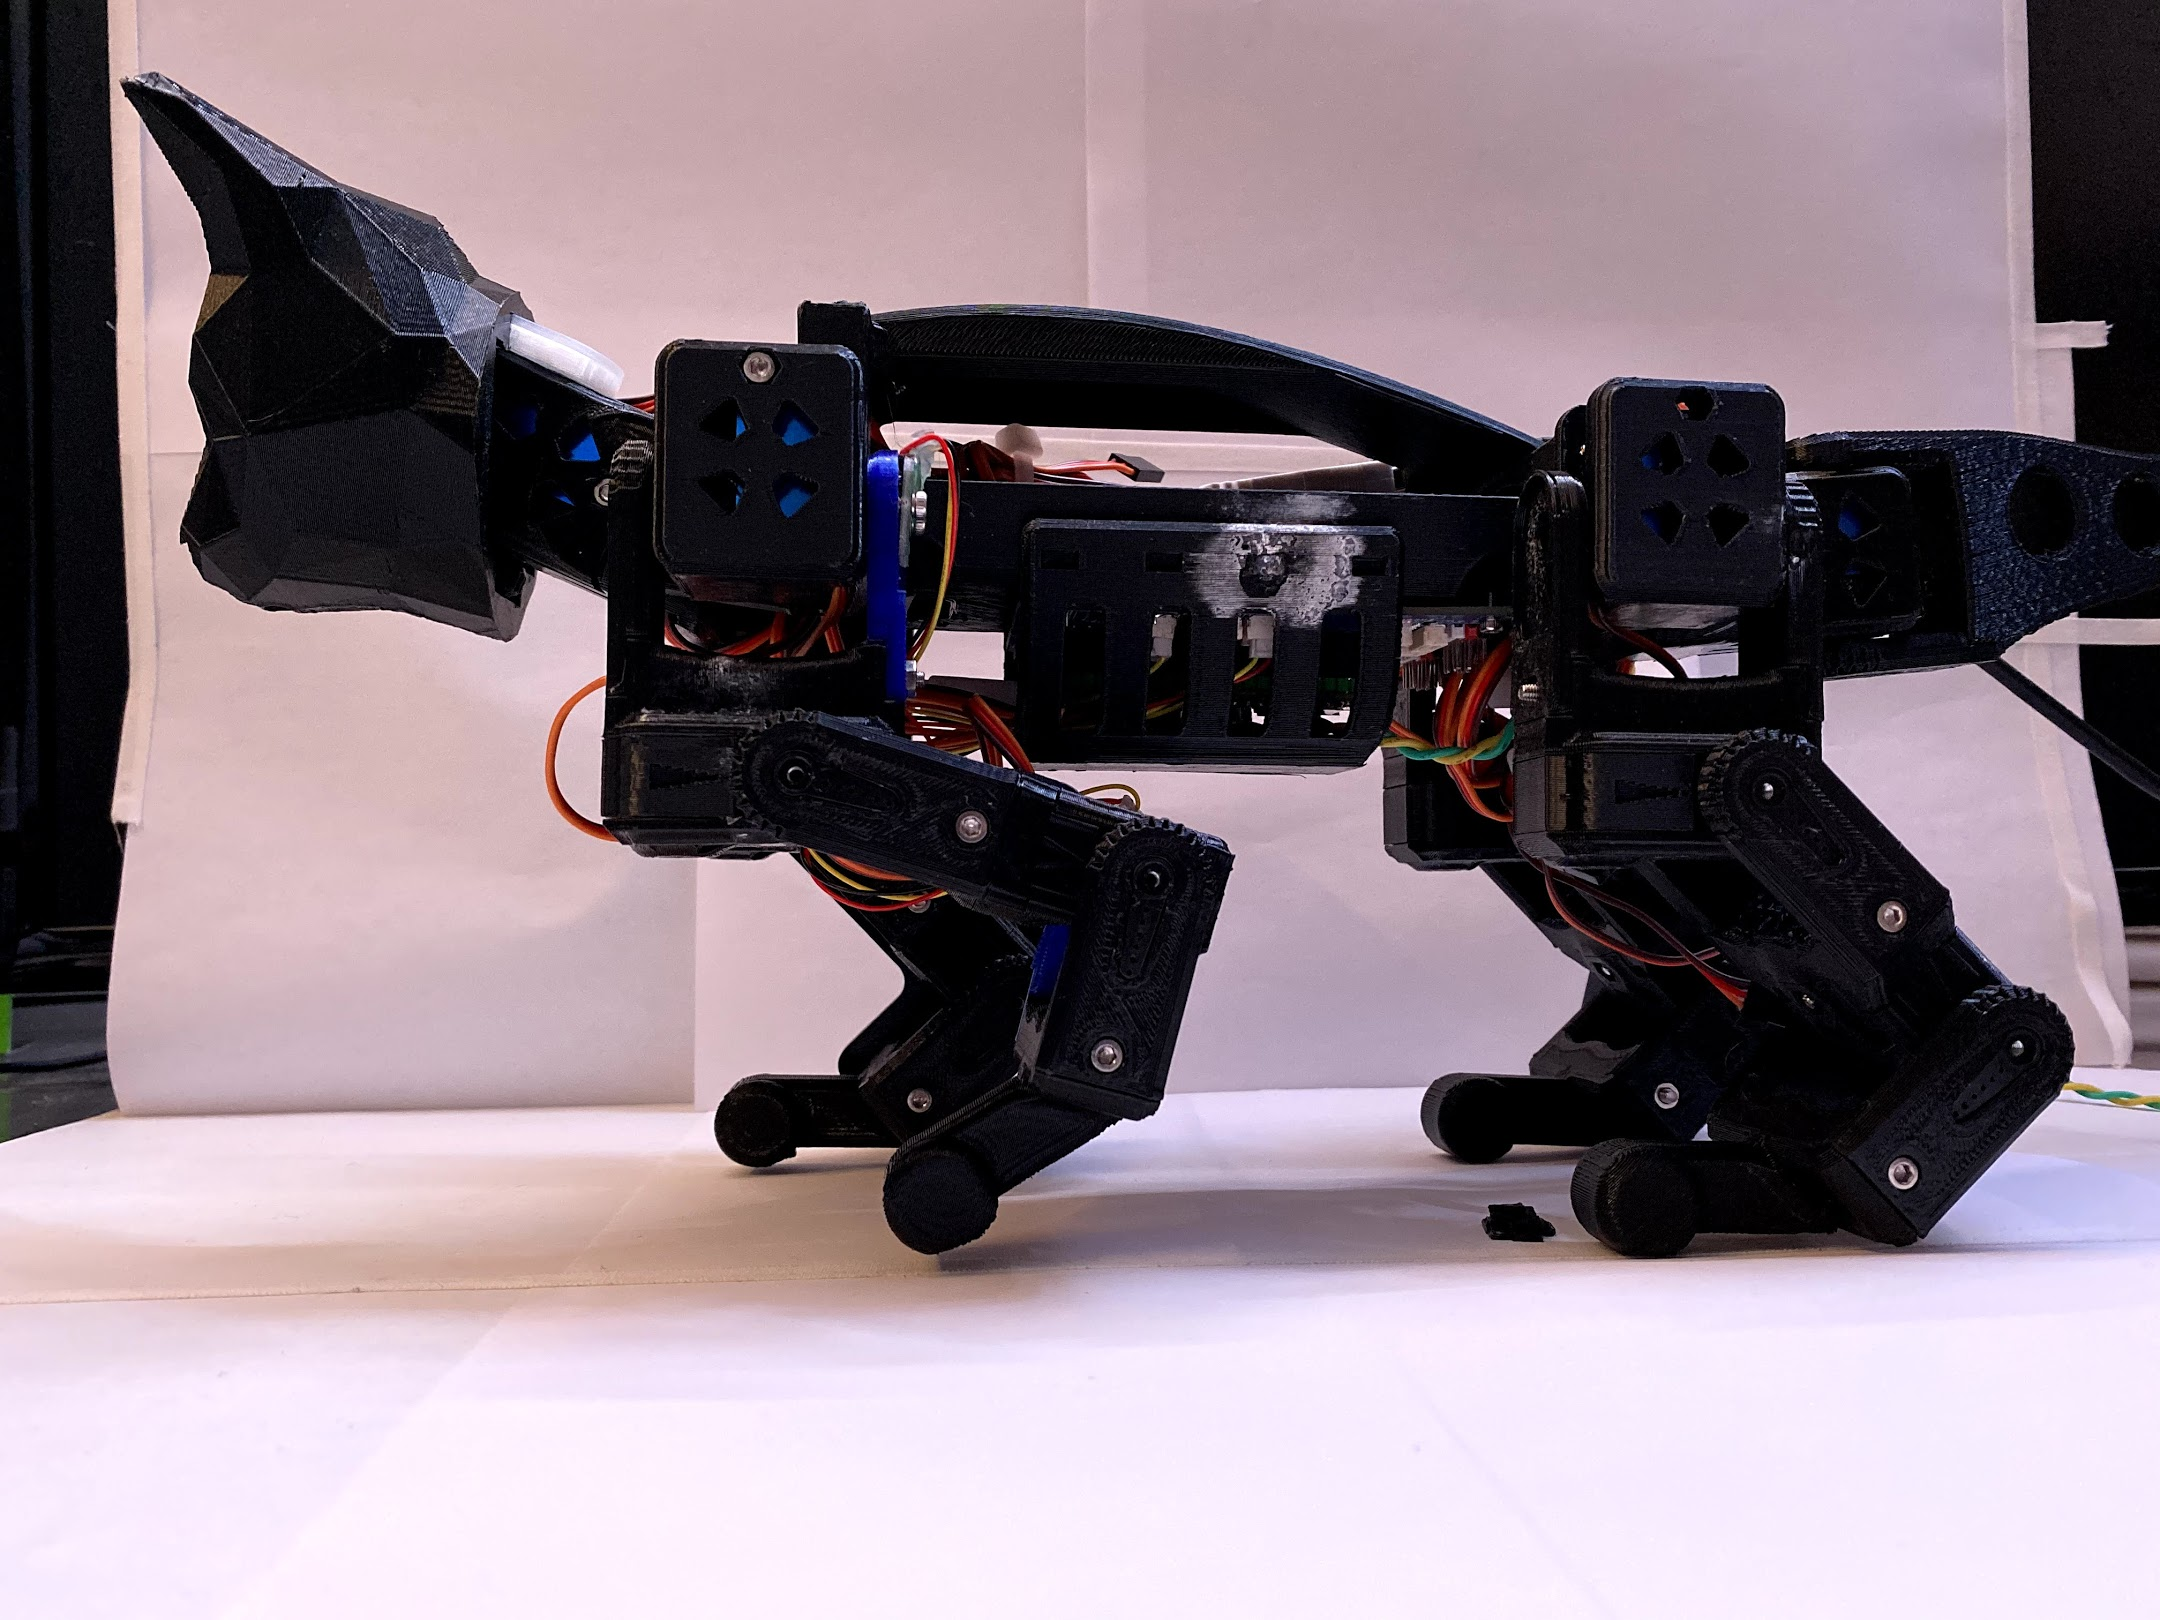
\includegraphics[width=0.24\textwidth]{Images/2.jpg}};
        \node[anchor=south west,inner sep=0] (im2) at (-4.2,-8) {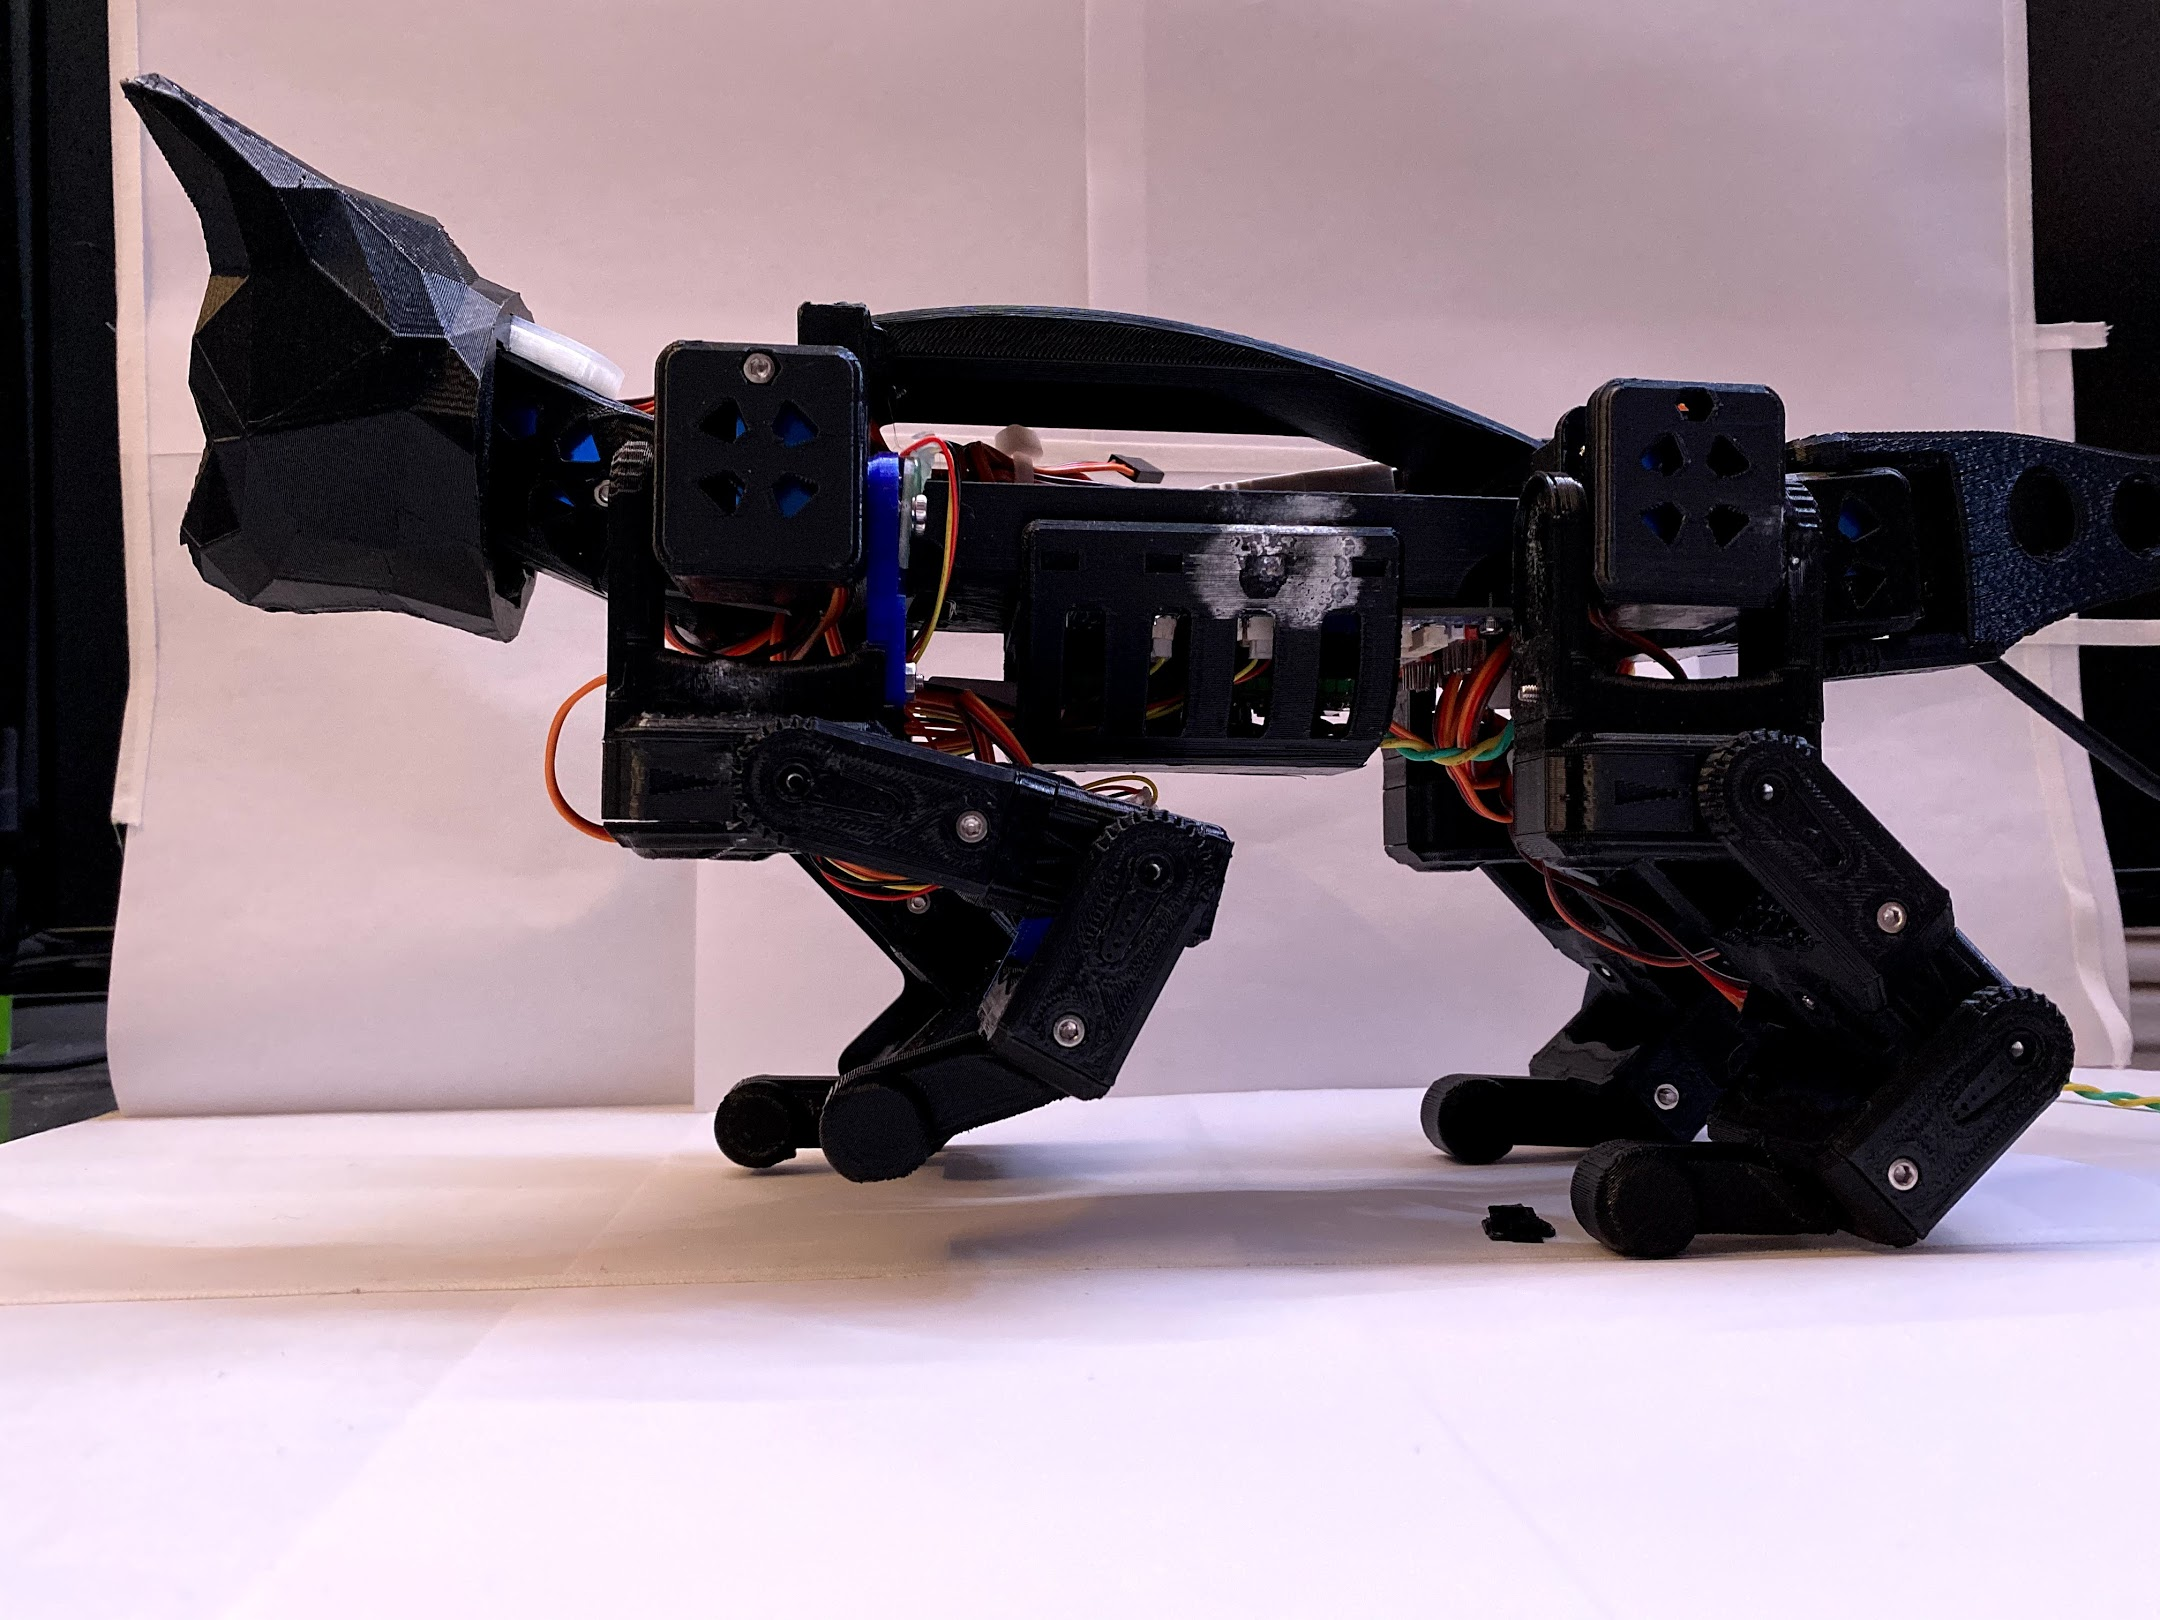
\includegraphics[width=0.24\textwidth]{Images/3.jpg}};
        \node[anchor=south west,inner sep=0] (im3) at (-0.4,-8) {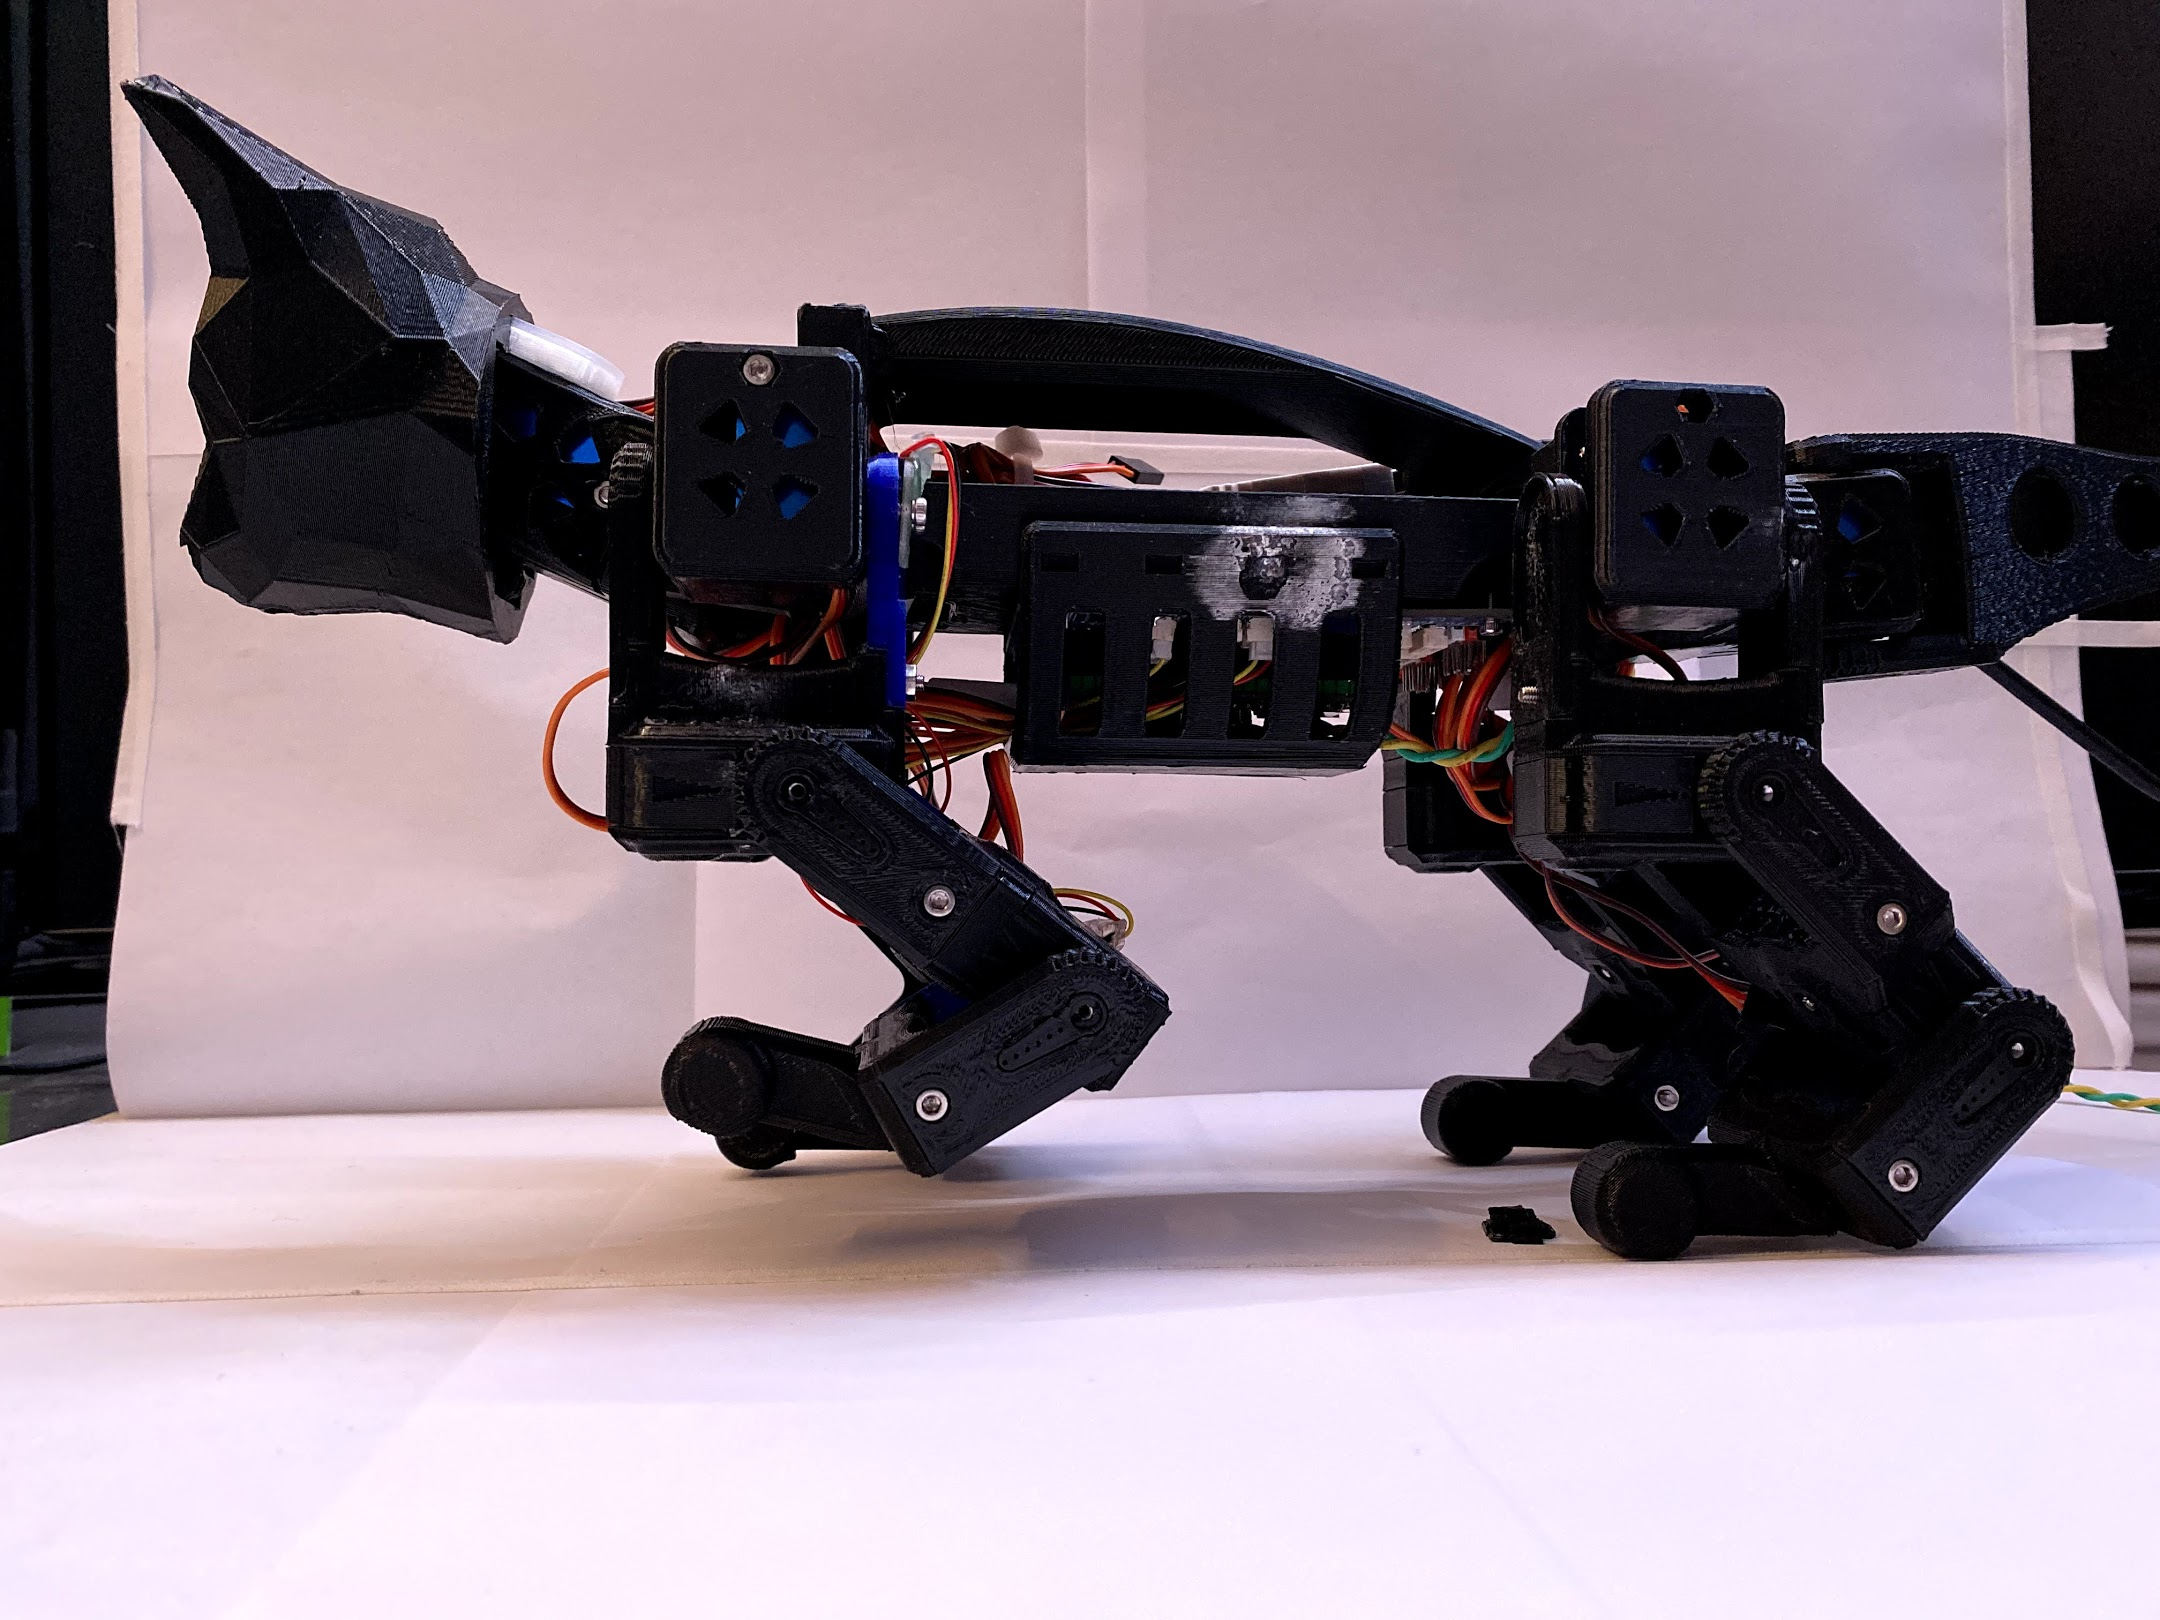
\includegraphics[width=0.24\textwidth]{Images/4.jpg}};
        \node[anchor=south west,inner sep=0] (im4) at (3.4,-8) {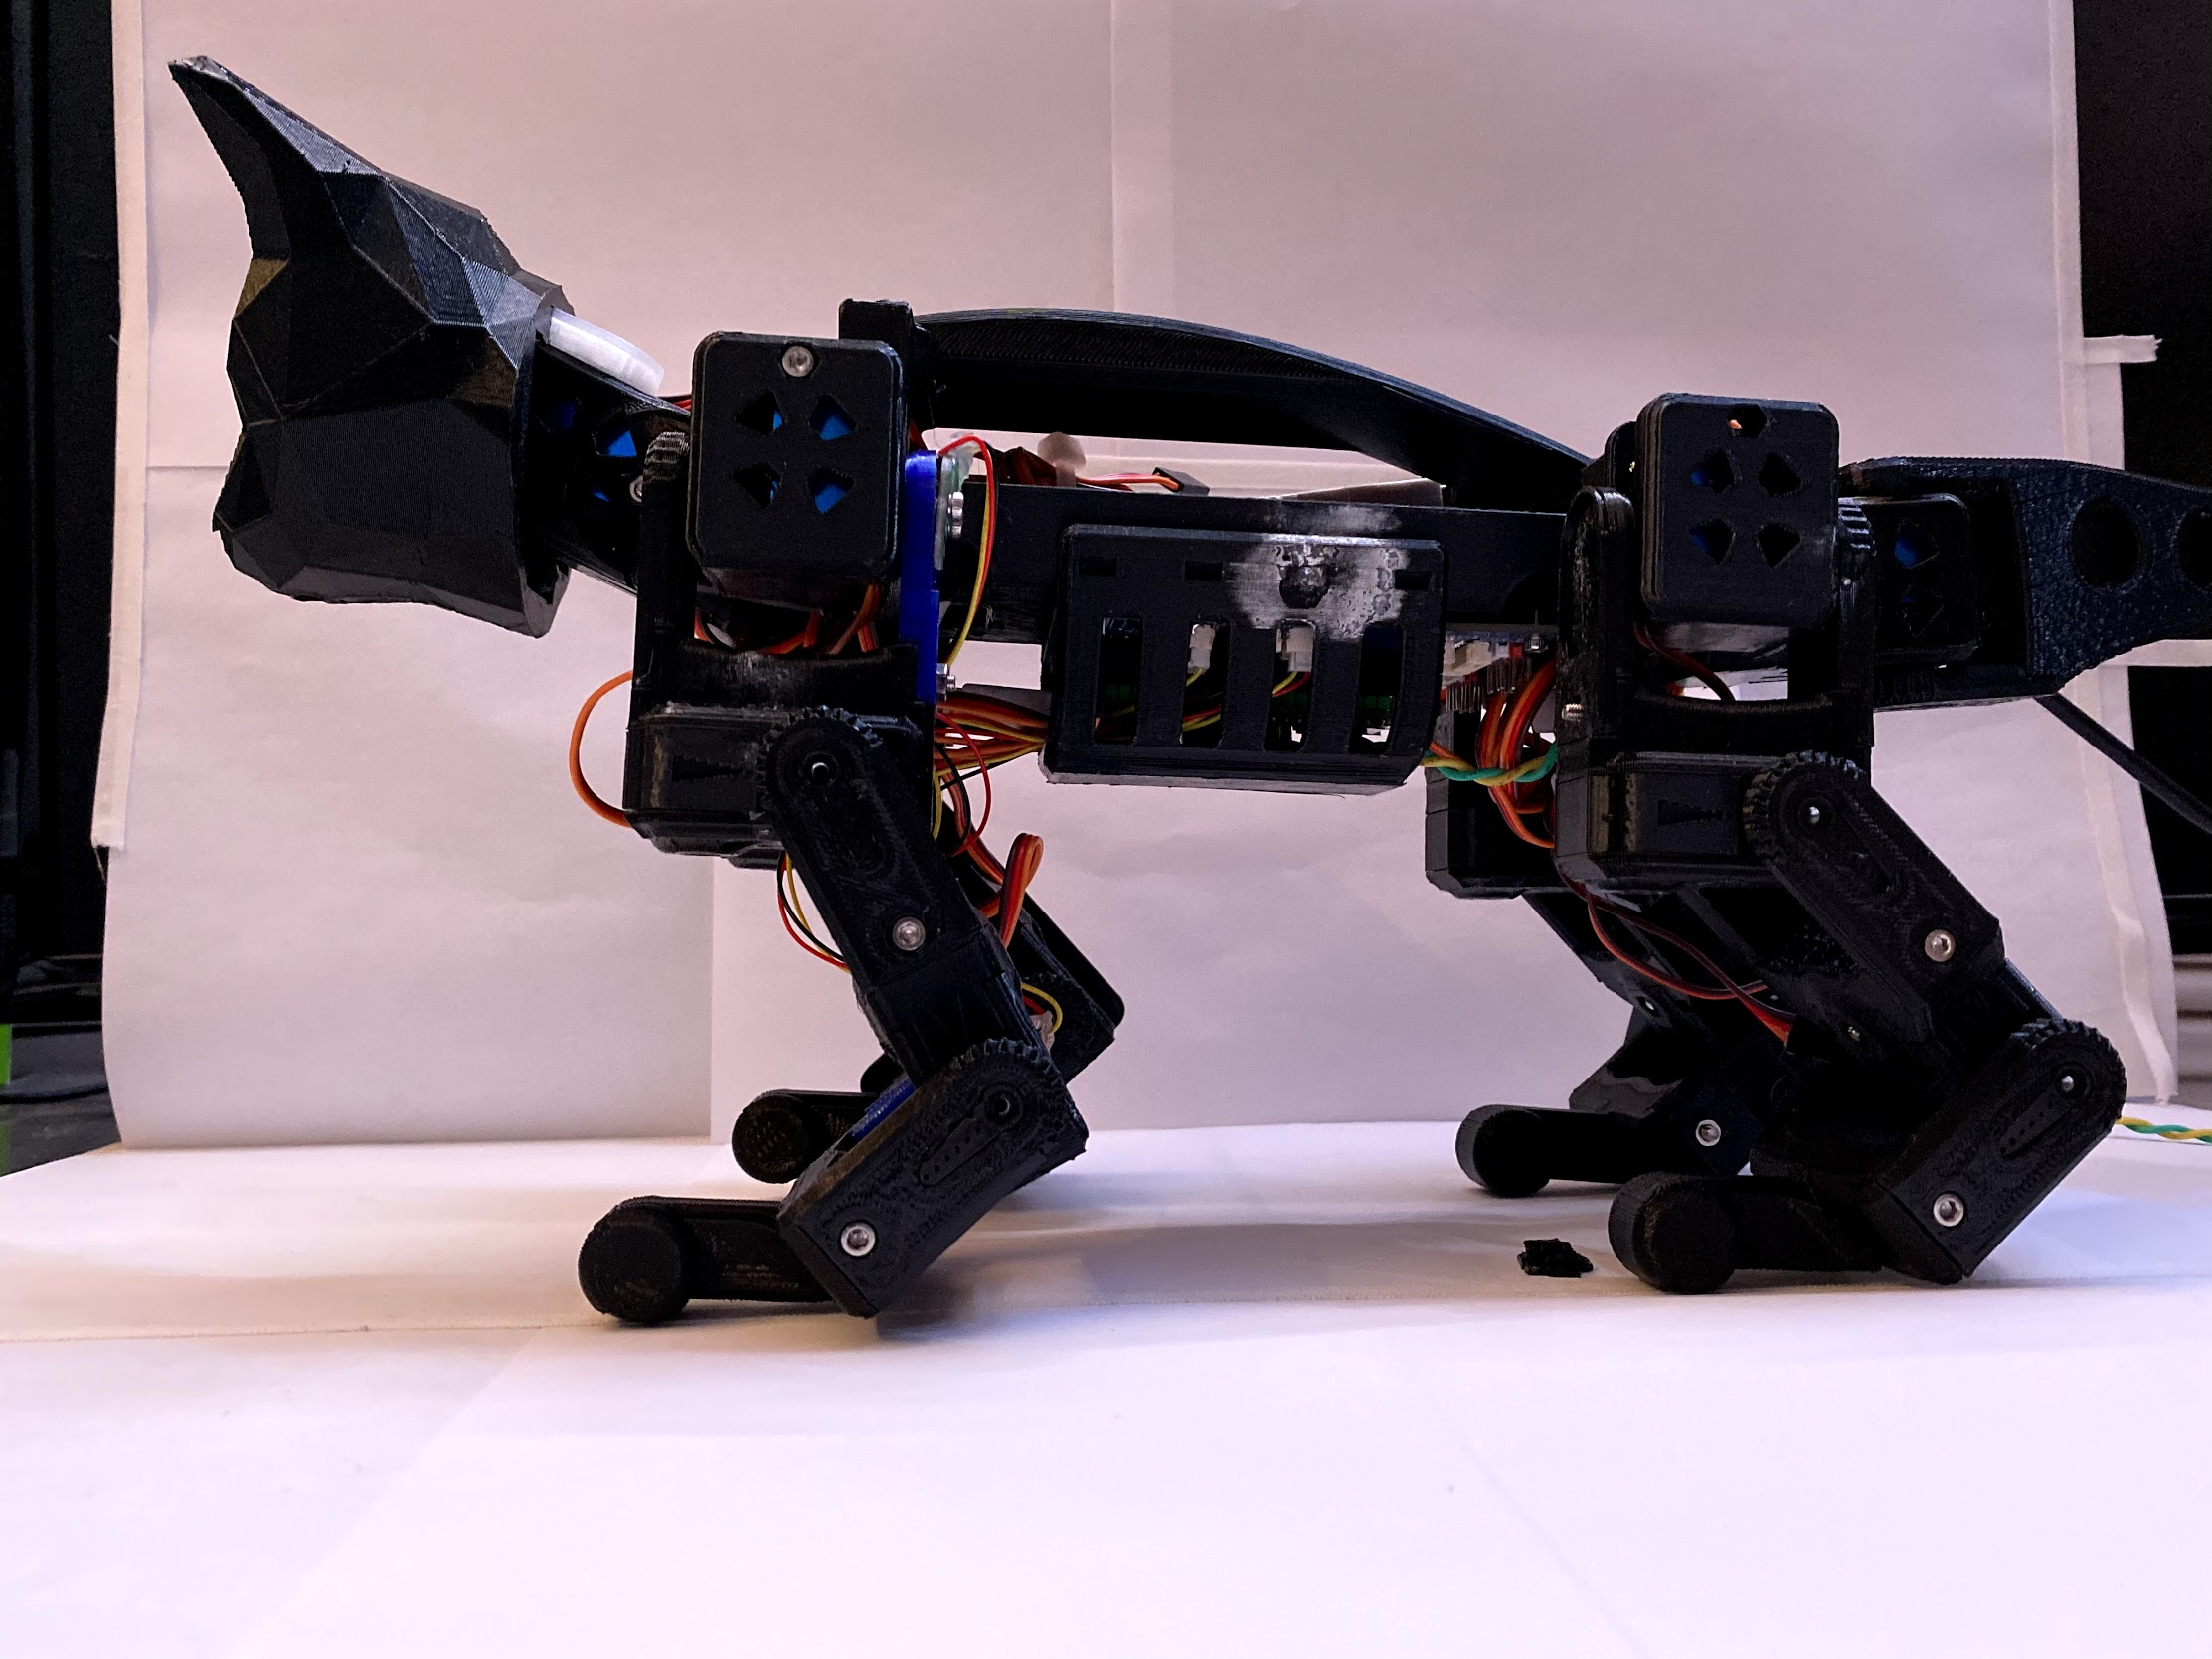
\includegraphics[width=0.24\textwidth]{Images/5.jpg}};

        \draw [very thick](-1,0.4) -- (0,0.4) -- (0,3.8) -- (-1,3.8) -- (-1,0.4);
        \draw [-latex,thick](-0.5,0.4)->(-0.5,-1.2);
        \draw [-latex,thick](-2.0,-4.15) circle (3pt);
        \draw [-latex,thick](-1.48,-1.5) circle (3pt);
        \draw [-latex,thick](-0.6,-1.45) circle (3pt);
        \draw [-latex,thick](-0.4,-4.1) circle (3pt);
        \draw [post,rounded corners=5pt](-2.09,-4.15)-|(-6,-5.3);
        \draw [post,rounded corners=5pt](-1.48,-1.58)-- ++(0,-30mm) -|(-2.2,-5.3);
        \draw [post,rounded corners=5pt](-0.6,-1.53)-- ++(0,-30mm) -|(1.6,-5.3);
        \draw [post,rounded corners=5pt](-0.32,-4.1)-|(5.4,-5.3);
        \draw[red,fill=red] (-6.43,-7.3) circle (1.25pt);    
        \draw[red,fill=red] (-2.73,-7.18) circle (1.25pt);    
        \draw[red,fill=red] (0.81,-7.1) circle (1.25pt);    
        \draw[red,fill=red] (4.45,-7.35) circle (1.25pt);    
        \end{scope}
    \end{tikzpicture}%
    \caption{Gait Generation as Shown on Robot}
    \label{fig:finalMotion}
\end{figure}

\section{Limitations}
There are a number of limitations of this system to this system primarily due to the choice of motors used. The chosen hobby servos have limited torque, slow speed and relatively slow update frequency of only \approximately330Hz. These limitations limit the size of the platform being maxed out at its current size with a very minimal payload capability. In addition to this without further sensor integration such as encoders for each limb, there is a limit to the possible accuracy of the platform. Despite these limitations the platform and its supporting architecture is capable of performing all required tasks and well as perform all necessary sub sections required in the reaching process. 
%%%%%%%%%%%%%%%%%%%%%%%%%%%%%%%%%%%%%%%%%%%%%%%%%%%%%%%%%%%%%%%%%%%%%%%%%%%%%%%%%%%%%%%%%%%%%%%%%%%%%%%%%


\chapter{Conclusion and Future Work}

This paper introduces the SmallKat robotic quadruped platform, the capabilities of the platform and the design criteria utilized when creating the platform. The resulting platform was capable of performing a number of educational concepts including kinematics, trajectory planning, gait generation, controls and dynamics. This platform can allow for institutions and research labs to develop and teach with a capable platform. This will assist in the development of multi-pedal systems in the field of robotics as a whole by creating more engineers with experience in the field.

The final platform is a combination of custom electronics and off the shelf servo motors. This combination allows for a reliable yet affordable platform. With the safety features integrated and the pedagogical objectives integrated into the design allow the system to be ideally suited for research and teaching within a lab setting. With most large quadruped platforms the robot has enough force to break itself or injure a user working on it, SmallKat has enough torque to walk but has safety features integrated and utilizes motors with low enough torque that it is unable to damage itself or the end user in any meaningful way. With this level of control the robot is still able to maintain a level of accuracy sub 3 mm at the end effector in the XYZ workspace.

As can be seen in the Section \ref{chap:Results} the robot designed is able to successfully and accurately perform all tasks required in the defined teaching objectives in Section \ref{sec:DesignReqs}. The resulting robot and simulation developed are able to perform static and basic dynamic walking gaits with optimal operator safety. The over all robot was designed to meet a low cost price point in order to make it feasible as a lab kit for colleges and universities to further expand their course offerings. The targeted price point for the completed system including charging, battery and all related electronics similar to that of the turtle bot Burger being \approximately\$550. Both robots operate in a similar environment, both focusing on the educational and the research and development space.

\section{Future Work}
%%%%%%%%%%%%%%%%%%%%%%%%%%%%%%%%%%%%%%%%%%%%%%%%%%%%%%%%%%%%%%%%%%%%%%%%%%%%%%%%%%%%%%%%%%%%%%%%%%%%%%%%%

\appendix
\singlespacing

%%%%%%%%%%%%%%%%%%%%%%%%%%%%%%%%%%%%%%%%%%%%%%%%%%%%%%%%%%%%%%%%%%%%%%%%%%%%%%%%%%%%%%%%%%%%%%%%%%%%%%%%%
\bibliographystyle{IEEEtran}
\bibliography{bibliography}

\end{document}